% REMEMBER: You must not plagiarise anything in your report. Be extremely careful.
\documentclass{l4proj}

    
%==============================================================================
% Put any additional packages here
% You can add any packages you want, as long as it does not alter
% the overall format (e.g. don't change the margins or the reference style).
%
\usepackage{pdfpages} % if you want to include a PDF for an ethics checklist, for example
%
%

\newcommand\TODO[1]{\textcolor{red}{TODO: #1}}

\begin{document}

%==============================================================================
%% METADATA
\title{The Evenir Case Files: A Text-Based Game Designed to Develop Historical Thought}
\author{Ivo de Vero}
\date{April 2, 2021}

\maketitle

%==============================================================================
%% ABSTRACT
\begin{abstract}
    %Every abstract follows a similar pattern. Motivate; set aims; describe work; explain results.
    %\vskip 0.5em
    %``XYZ is bad. This project investigated ABC to determine if it was better. 
    %ABC used XXX and YYY to implement ZZZ. This is particularly interesting as XXX and YYY have
    %never been used together. It was found that  
    %ABC was 20\% better than XYZ, though it caused rabies in half of subjects.''
    
    Designing an intervention which can effectively develop critical thinking skills is challenging because of the problems of transfer and domain specificity. This research project designed and developed a text-based game in React which could teach important critical thinking skills in the domain of history in its players. This was done by combining Schon's Reflective Practitioner model together with game-based learning principles. This contributes to the existing literature because the combination of the models employed allowed the study design to address the problem of transfer, as well as developing critical thinking skills. The instrument used to evaluate the effectiveness of the game was a questionnaire based on the Reflective Practitioner model. The gathered qualitative data was analysed through affinity diagramming. The results show that the game that was developed has the potential to encourage advanced levels of historical thought. However, more work needs to be done before conclusions about the long-term efficacy of this intervention can be drawn. 
\end{abstract}

%==============================================================================
%% ACKNOWLEDGEMENTS
%\chapter*{Acknowledgements}
% Enter any acknowledgements here. This is optional; you may leave this blank if you wish,
% or remove the entire chapter
%
% We give thanks to the Gods of LaTeX, who in their eternal graciousness, 
% have granted that this document may compile without errors or overfull hboxes.
%

%==============================================================================

% EDUCATION REUSE CONSENT FORM
% If you consent to your project being shown to future students for educational purposes
% then insert your name and the date below to  sign the education use form that appears in the front of the document. 
% You must explicitly give consent if you wish to do so.
% If you sign, your project may be included in the Hall of Fame if it scores particularly highly.
%
% Please note that you are under no obligation to sign 
% this declaration, but doing so would help future students.
%
\def\consentname{Ivo de Vero}
\def\consentdate{2 April 2021}
\educationalconsent



%==============================================================================
\tableofcontents

%==============================================================================
%% Notes on formatting
%==============================================================================
% The first page, abstract and table of contents are numbered using Roman numerals and are not
% included in the page count. 
%
% From now on pages are numbered
% using Arabic numerals. Therefore, immediately after the first call to \chapter we need the call
% \pagenumbering{arabic} and this should be called once only in the document. 
%
%
% The first Chapter should then be on page 1. 

% PAGE LIMITS
% You are allowed 40 pages for a 40 credit project and 30 pages for a 
% 20 credit report. 
% This includes everything numbered in Arabic numerals (excluding front matter) up
% to but *excluding the appendices and bibliography*.
%
% FORMATTING
% You must not alter text size (it is currently 10pt) or alter margins or spacing.
% Do not alter the bibliography style. 
%
%==================================================================================================================================
%
% IMPORTANT
% The chapter headings and structure here are **suggestions**. You don't have to follow this model if
% it doesn't fit your project. Every project should have an introduction and conclusion,
% however.  If in doubt, your supervisor can give you specific guidance; their view takes precedence over
% the structure suggested here.
%
%==================================================================================================================================
\chapter{Research Background and Motivation}
% reset page numbering. Don't remove this!
\pagenumbering{arabic} 

\section{The Challenges of Teaching Critical Thinking}

There is an abundant literature on the importance of critical thinking (CT) going back decades. \citet{hunt1995will} argued that the global economy had entered a new phase which required a new kind of worker, the “knowledge worker”, who would be capable of manipulating “abstract and complex symbols and ideas” and could “remain flexible enough to recognise the need for continuing change” \citep{hunt1995will}. As a result of surging demand for the knowledge worker, any country which wished to remain competitive in the global marketplace would need to reform its education system to emphasise CT: that combination of skills and attitude that would form the knowledge worker \citep{hunt1995will}. Two decades later, Western educators continue to emphasize the importance of CT for the success of the next generation and lament current institutional barriers to teaching it \citep{davies2016ct, Staton2021ct}. \citet{halpern1998teaching} noted that an absence of the CT also has negative repercussions for people in their personal lives, not just their career. A substantial part of the American population, Halpern pointed out, spent more money than they could afford to do on psychics and pseudo-scientific remedies \citep{halpern1998teaching}. This too has not appeared to improve substantially in the past two decades: \citet{mclaughlin2017explicitly} note that belief in pseudo-historical narratives around ancient civilisations, such as the Maya, can negatively impact the well-being of their contemporary descendants. Conspiracy theories have been part and parcel of American political discourse for several years now with potentially dire implications for the health of its democracy \citep{venka2020QAnon}. Thus, the difficulty of teaching CT appears to be a pervasive problem with global reach and sufficient complexity to continue to challenge educators and academics alike. 

In a comprehensive literature review of the major academic contributions to the subject of CT, \citet{lai2011critical} describes three areas of agreement among scholars of the different contributing fields. First, that CT has a skill component. These are abilities such as analysis, inference, evaluation and problem solving \citep{lai2011critical}. Second, CT has a dispositional or attitudinal component. CT dispositions are “consistent internal motivations to act toward or respond to persons, events, or circumstances in habitual, yet potentially malleable ways” \citep{facione2000CT} and include traits like open and fair-mindedness, inquisitiveness, and the desire to be well-informed \citep{lai2011critical}. Finally, there is agreement on the fact that background knowledge is a prerequisite for effectively employing CT. This is because the evidence, reasonings and explanations that are considered to be examples of CT are domain-specific \citep{lai2011critical}. 

The interplay between these three components is what makes teaching CT so challenging. \citet{facione2000CT} note that having CT skills does not correlate with a disposition towards applying CT, although there is a correlation between disposition and proficiency with CT skills. Attention must be paid to both for there to be an improvement in students. Furthermore, \citet{willingham2008critical} highlights that once students have been trained to think critically in one domain, they do not automatically do so in others. Even within the same broad domain such as mathematics or history, if students are taught to apply critical thinking to one specific type of problem, and then encounter a problem of a different type, there is no guarantee that those CT skills will transfer over to the new problem \citep{willingham2008critical}. The importance of domain knowledge is such that the most effective CT interventions are those where it is taught in the context of a specific discipline, an observation also supported by \citet{lai2011critical}. The next sections of this chapter will elaborate on how this research project aims to address the problems raised by domain specificity, CT skills and CT dispositions. 

\section{Critical Thinking in the Domain of History}

Because of the fundamental challenge of transferring CT skills from one domain to another described in the literature of the previous section \citep{lai2011critical, willingham2008critical}, the author decided to restrict the scope of this research project to one domain, the discipline of history. There is a literature which shows that history can engage both the dispositions and skills necessary to think critically, making it a useful domain to focus on.

\citet{yogev2013need} argues that CT should be considered a fundamental part of the discipline because of the role it plays in forming citizens who actively engage with their democracy. Societal trends like the consumption of information through scattered media sources and the fragmentation of society into smaller communities further increases the challenge of developing “historical consciousness” in students \citep{yogev2013need}. Clear in this argument is the implicit belief that teaching students history will encourage them to think critically about broader issues, or in other words, increase student disposition to think critically. \citet{mclaughlin2017explicitly} view history as a particularly appropriate domain to boost the CT skills of students because of the type of thinking the field demands of its scholars. Indeed, the example \citet{halpern1998teaching} gives to illustrate a critical thinking task is of weighing the relative credibility of two sources, which is an integral part of the work of the historian, as the rest of this section will illustrate. Since this literature has shown that history is a useful microcosm of the challenges faced in the broader field of CT education, it is important to first understand what evidence, reasonings and explanations are valued by historians, before being able to design a study to address them.  

The process of the historian at work this section will outline is based on \emph{The Pursuit of History}, a successful book by \citet{tosh2006pursuit} marketed as the “essential introduction to the practice of history” \citep{tosh2006pursuit}. Therein, \citet{tosh2006pursuit} provide an overview of the academic discipline, but then spend the majority of their pages describing the process of the historian. This is something which sets the work apart from other renowned books on the subject by historians such as \citet{carr2018history}, which focus primarily on providing a definition of the discipline. 

The first step \citet{tosh2006pursuit} outline in the historian’s process is what they term “external criticism”. This involves checking the authenticity of a historical document in the sense of verifying the truthfulness of its geographical and temporal details, to guard against forgery. The second step of the process is “internal criticism”, or actually interpreting the document the historian is working with, which the authors note is “usually much more demanding”. Here, the historian must consider what influenced the author of a document at the time of writing, as well as the concept of bias, that is the intended purpose of the document at the time and the deliberate or unconscious distortions in the text that could have caused. This can lead to “gaps in the record”, missing or obscured pieces of information in an otherwise consistent story told by a group of historical documents, and can affect even seemingly objective sources such as statistical reports. The historian must thus weigh sources against each other, analysing their relative merit to the question they are investigating or constructing around the historical documents at their disposal. Tosh and Lang note that internal criticism requires “a knowledge of historical context and insight into human nature”. This is where “historians come into their own” \citep{tosh2006pursuit}. 

There should be no doubt at this point that historians must exercise CT to be successful. \citet{tosh2006pursuit} themselves summarise the process of the historian by calling it “common sense applied very much more systematically and sceptically than is usually the case in everyday life, supported by a secure grasp of the historical context and, in many instances, a high degree of technical knowledge”. Thus, the process here outlined is the domain-specific CT that is the focus of this research project, what \citet{willingham2008critical} noted would in layman terms be called “thinking historically”. 

\section{The Reflective Practitioner}

The theoretical framework the author selected as a basis for the study design of this research project is provided by \citet{schon1984reflective} in his highly influential book \emph{The Reflective Practitioner}. Schon was studying a crisis he had observed in the American professions, which felt that they were ill-equipped to deal with the challenges posed by the developments in the Cold War period in the workplace and in society. He argued that higher education institutions were unable to meet these new challenges because they were rooted in a conceptualisation of knowledge he dubbed ‘Technical Rationality’ (TR) \citep{schon1984reflective}. TR viewed professional activity as problem solving based in scientific theory and methodology. It was a consequence of Positivism, the leading philosophical school of thought in the nineteenth and early twentieth century, which put forth the pre-eminence of empirical science over any other form of knowledge and sought to rationalise all aspects of human society and was highly influential in universities \citep{schon1984reflective}. However, Schon argues that the great limit of the TR model was assuming problems as given. In a real-world context, problem setting was as important as problem solving. The act of defining the problem at hand and framing it in a certain context is not a technical process, as there is too much uncertainty around the variables at play to derive them from applied science. To be effective, if a practitioner cannot rely on scientific principles to define and frame a problem they face, they must look for an alternative source of knowledge. 

Schon describes this source of knowledge as the ‘Reflective Practitioner’ (RP) model. The core of the RP model is the concept of “knowing-in-action” \citep{schon1984reflective}. \citet{schon1984reflective} describes this as spontaneous “actions, recognitions and judgements” performed by the practitioner. The practitioner is often unaware of having learned how to perform, and is typically unable to describe the knowledge implicit in their actions. One of the examples Schon offers is of a baseball player getting “into the groove” \citep{schon1984reflective}, almost instinctively knowing what to do during a game, but afterwards unable to describe why they felt their actions were correct. He showed through his studies of a broad range of practitioners, ranging from architects to therapists, that this concept of “knowing-in-action” was common across all of them, and is one of the key things which distinguishes the RP model from the principles-first approach of the TR model. 

The other key difference between the RP and TR models of knowing is the process of problem solving. In the TR model this is a technical process which follows scientific methods of problem setting with fixed variables. On the other hand, The RP model argues that problem solving is a combination of experience and technical know-how. A practitioner does not assume a problem as given. Instead, they aim to identify the particular features of the specific problem they are working on by reflecting on what they can observe and on their previous experience solving similar problems. \citet{schon1984reflective} defines this as “seeing-as”, in other words, framing a new problem in the context of everything they have learned solving past problems. Once a practitioner can relate a new problem to past experience, then they can “do-as” \citep{schon1984reflective}, applying what they know to the new problem, even if they cannot describe what it is that they’re seeing-as and doing-as. 

\citet{halpern1998teaching} notes that CT skills are also known as “higher order” cognitive skills in order to highlight their complexity. She further goes on to explain that CT skills are needed in real life to deal with “complex issues and messy, ill-defined problems” \citep{halpern1998teaching}. Although Schon was not writing in the context of CT education, the parallels between the RP model and the effective application of CT are striking. It seems highly likely that a practitioner seeing-as and doing-as must exercise some measure of CT to be successful in their tasks. That implicit recognition of the connection between CT and how practitioners operate could also be part of why CT skills have often been discussed in relation to employment. \citet{willingham2008critical} also notes that for a student to improve their CT abilities, practice is key, which further reinforces the connection. An important implication of this connection for this research project is that if a practitioner can be brought to think critically about a problem, by the RP model this should extend to different types of problems as long as that practitioner can "see-as", or in other words relate the new problems to the old ones they have already solved. This is central to the design of this project detailed in the next two chapters. 

That the RP model captures the work of the historian is also evident. The process outlined by \citet{tosh2006pursuit} in the previous section has no formula to be systematically applied for a given set of similar historical problems. Subjecting unique sources to rigorous external and internal criticism, as outlined in the previous section, implies treating each problem as new, then critically observing and reflecting. Thus having brought together the literature on CT education, history, and reflective practice, part of the objectives of the research project can now be stated. This project aims to investigate history-specific CT skills and dispositions by applying the Reflective Practitioner model to Tosh and Lang’s overview of the historian’s process. 

\section{Game-Based Learning and its Advantages}

Traditional classroom interventions focussing on CT tend to concentrate on developing skills as opposed to increasing the disposition to think critically \citep{facione2000CT,willingham2008critical,lai2011critical}. A robust example of this type of intervention is reported by \citet{reed2001teaching}, who designed a college history module to explicitly teach CT skills together with history content, finding positive results. However, as \citet{facione2000CT} and \citet{willingham2008critical} highlight, CT dispositions need to be considered alongside skills for maximum impact. 

There is a literature which has consistently observed that videogames are a particularly effective medium for developing skills while maintaining a high level of motivation to do so in their players. For example, \citet{chowanda2016gamification} find statistically significant evidence that playing a history-themed game helped a group of secondary school students remain motivated throughout the class and remember names and timelines more effectively than their control group utilising textbooks. A particularly valuable perspective is further offered by \citet{barr2019graduate}, who runs a randomised controlled trial to measure learning gains of more abstract skills such as communication and adaptability in a game-playing intervention group composed of university students. Not only does Barr find statistically significant learning gains, he also follows up the experiment with interviews, and the qualitative feedback provides evidence of a learning experience which was also engaging and entertaining \citep{barr2019graduate}. Skills such as adaptability, and the factor of motivation, are crucial components in CT disposition, considering their definition as “consistent internal motivations” to exhibit certain behaviours \citep{facione2000CT}. It should be noted that the field of game-based learning (GBL) and gamification suffers from a lack of empirical studies, particularly across examples or over time, to be able to quantitatively say how much more effective games and gamification are in learning \citep{seaborn2015gamification} compared to other methods, and it would be well outside of the scope of this research project to attempt to do so. However, the quantitative and qualitative evidence in the literature that such gains can be had, regardless of their relative effectiveness, is persistent enough that this direction is worth exploring further, because addressing the key problem of the disposition to think critically appears more challenging to do with traditional CT interventions compared to videogames.  

The process whereby a videogame can teach skills while keeping a high level of motivation is elaborated in a seminal article by \citet{malone1980makes}, which outlines the three concepts of goals, fantasy and curiosity. Goals are the objective of the game, what it is that the player seeks to accomplish. A game goal which is clear and compelling is an intrinsic motivator because the player will be driven to complete it for its own sake. Fantasy refers to the concept of suspension of disbelief, when a game presents images and situations of any kind which are “not present” in reality \citep{malone1980makes}. Malone differentiates between extrinsic and intrinsic fantasy. In a learning context, games which have an intrinsic fantasy present images and situations related to the types of skills the game is trying to teach. This means that “problems are presented in terms of the elements of the fantasy world” \citep{malone1980makes}. Malone believes this type of fantasy to be the most effective, as they better suggest how a skill could be used to accomplish a real-world goal \citep{malone1980makes}. Games in which present situations tightly related to the skills they try to teach allow players to “exploit analogies between their existing knowledge of the fantasy world and the unfamiliar things they are learning” \citep{malone1980makes}.  Malone divides the third concept, curiosity, in sensory and cognitive curiosity. Sensory curiosity is a technique to attract and retain the attention of players by changing the sensory stimuli of the game environment \citep{malone1980makes}. Cognitive curiosity, however, is defined as “a desire to bring better form to one's knowledge structures” \citep{malone1980makes}. This type of curiosity is a powerful intrinsic motivator because it relies on an instinctive need of the player to uncover information. The game designer can harness this by presenting information which challenges the existing game knowledge of the players. For Malone, these three concepts make videogames a fertile terrain to harness “intrinsic motivation”, that is, the desire to do something, such as learning, for its own sake. As such, they are what shaped the educational side of the game design decisions made in the development of the research product used to conduct the research in this report, which will be detailed in the next chapter. 

\section{Combining the Literatures - Study Aims}

Having introduced the literatures which inform the motivation, background and development of this research project, it is now possible to restate its goals in full and summarise what has been discussed so far. This project aims to develop a game harnessing GBL principles to strengthen CT skills and dispositions in the context of the discipline of history. 

There are two contributions this research project seeks to make which contribute to the existing literature on GBL. The first crucial differentiator is the employment of the Reflective Practitioner model of behaviour in the context of a GBL-based CT intervention. The insight Schon brings is that because practitioners learn by drawing on previous experience, then a game explicitly designed to boost CT skills and dispositions in a practitioner should form part of that experience. This means that the results of this research project should be able to say something about the long term gains in players, which a quantitative or mixed method struggles to do unless employed over a long period of time. 

Second is the key theoretical link between the idea of internal motivation as expressed by Malone (1980) as a factor which encourages people to play games and the idea of motivation as a set of consistent internal behaviours described by \citet{facione2000CT} in the context of developing CT skills. Most academic work which discusses GBL and CT together highlights the advantages games offer to skills development but somewhat neglect the equally important side of CT dispositions (see \citet{mccall2013gaming} and \citet{mccall2016teaching} for a review of such literature in the field of history, for example). 

\chapter{Developing the Research Product}
\section{Process Overview}
\subsection{Motivating the Content of the Game}

The game the author of this research project developed is titled Evenir Case Files. In the game, the player takes on the role of a Keeper of Records serving the Mage Council of the fantasy kingdom of Evenir. The game is entirely text-based, the only illustrations present are menu icons. The first screen of the game introduces the player to the fantasy world of the game and explains their task. As Keeper of Records, the Council asks the player to investigate the sealing of an ancient witch and establish whether it was the correct thing to do, as the court historians of the king of Evenir claim. The first screen also hints that the player is descended from the witch, another reason why the Council selected the player specifically. After that introduction, the game is played by navigating to different screens, representing locations in the world, which contain documents to be read. There is a timer, initially set at thirty days, and visiting a location as well as reading documents removes days from the timer. Once the player has no more days to act with, they must drag individual sentences from the documents they have read into three sections which require them to think about what that sentence contributes to their overall argument. Once the player presents their case, they are taken to a final screen where the Council makes a statement on the quality of their case. The rest of this section will show that the presentation and mechanics of the game are grounded in the literature this research project draws on, and are specifically constructed with the aim of developing CT skills in history. 

\begin{figure}[htb]
    \centering
    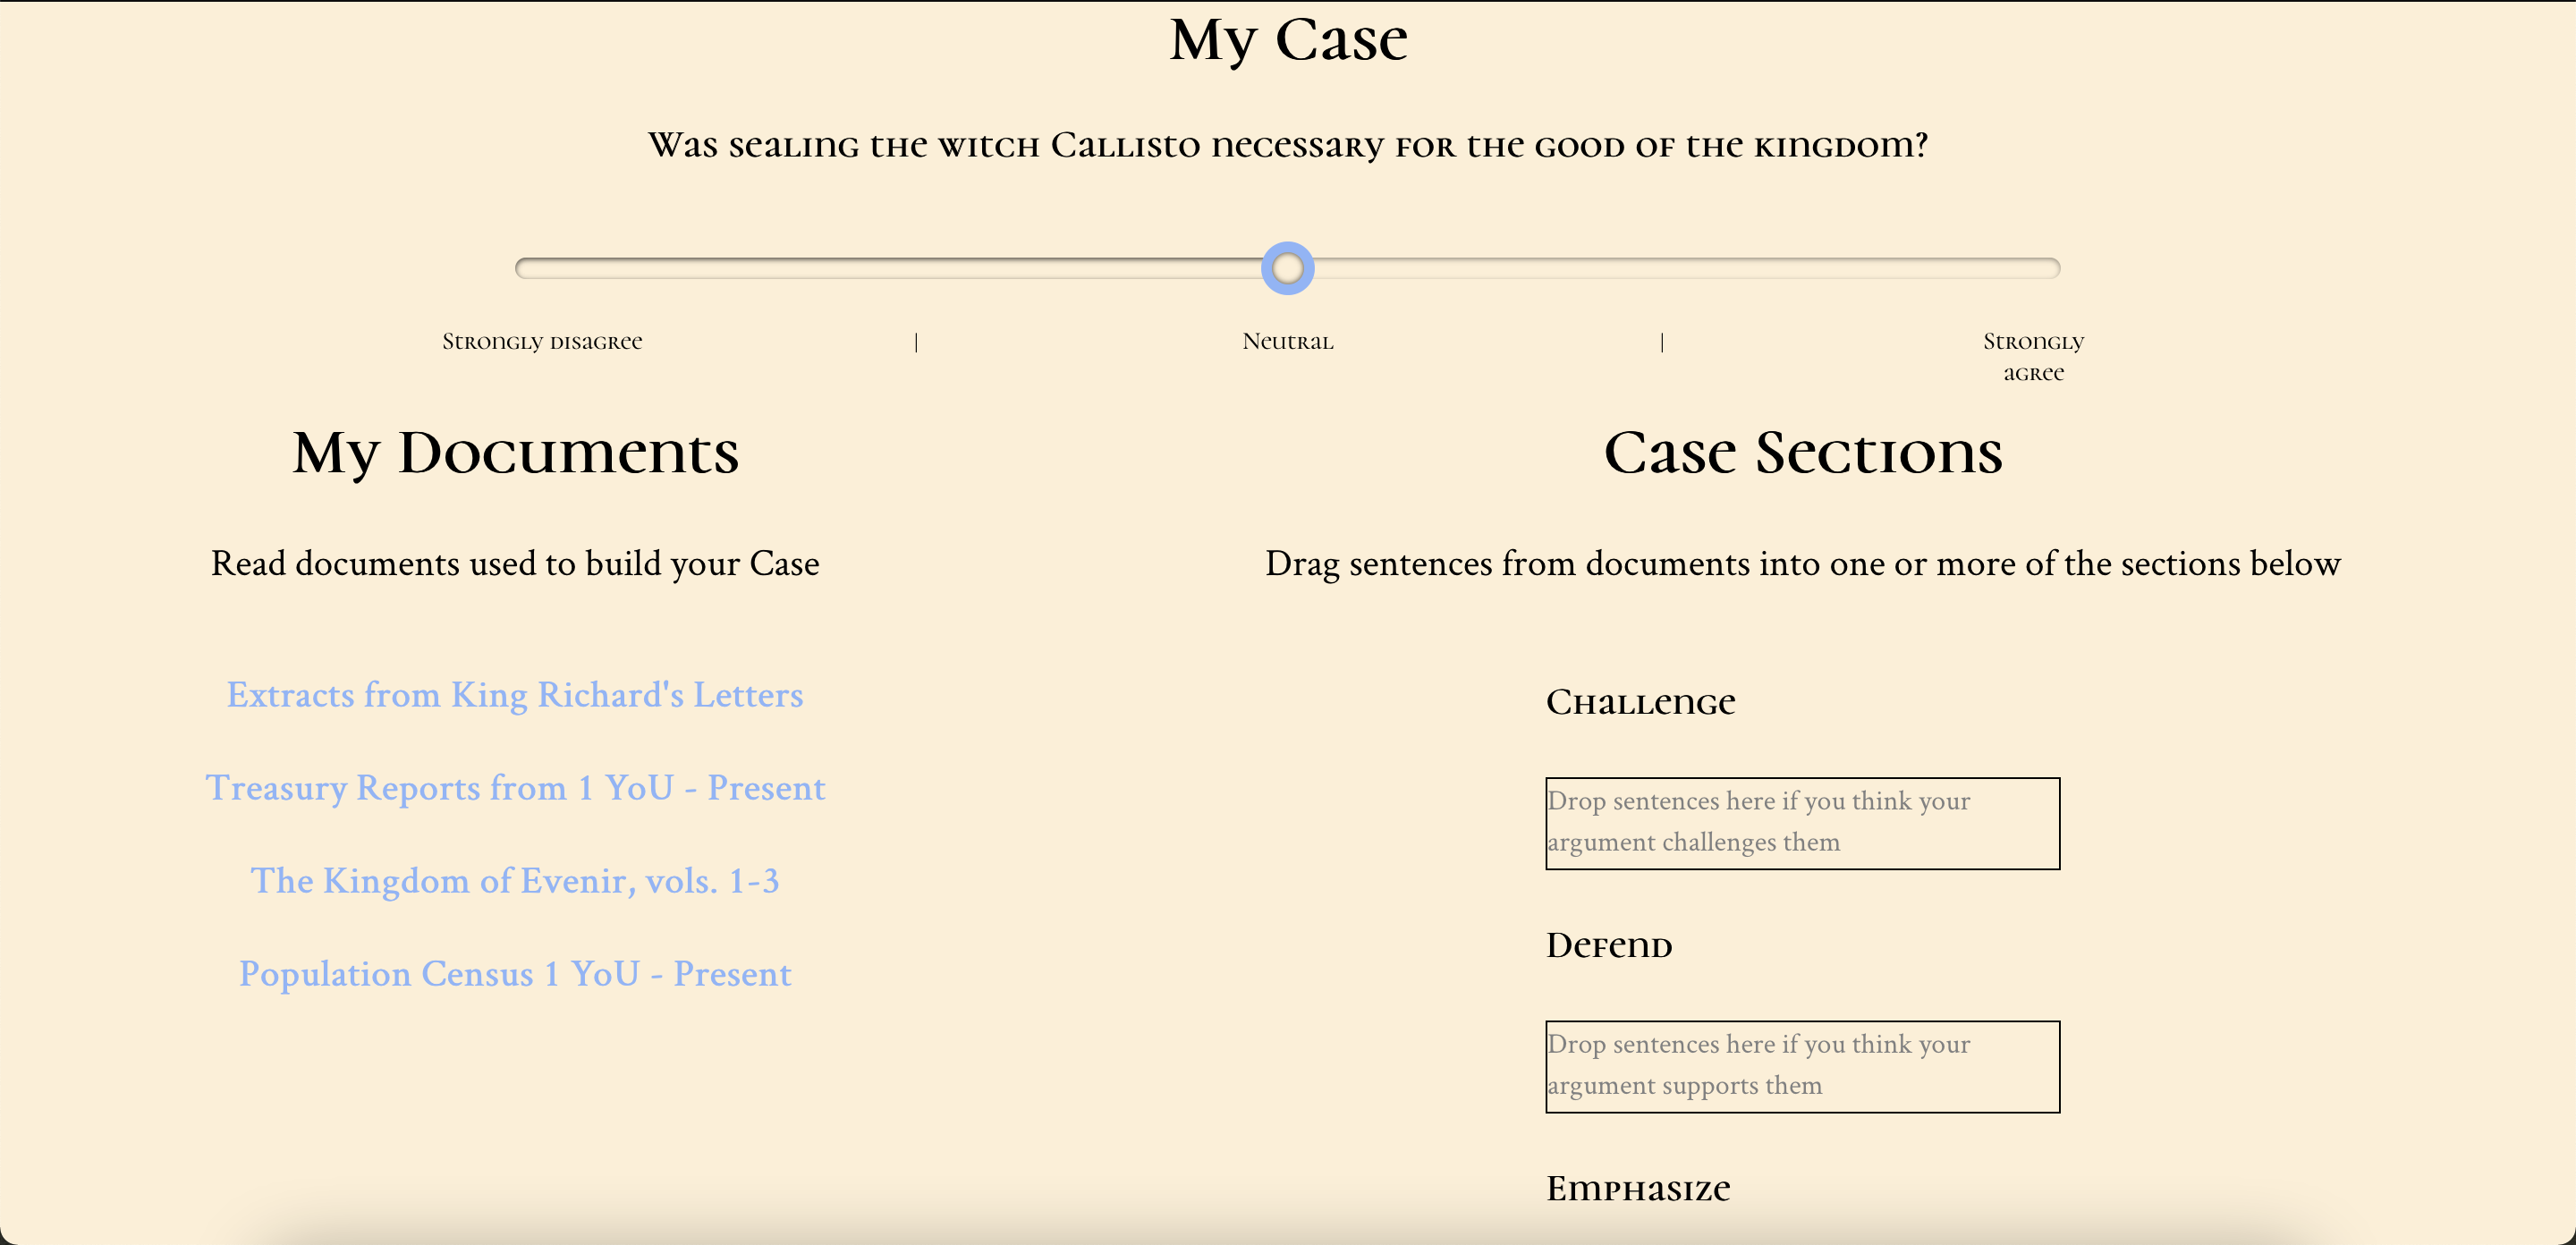
\includegraphics[scale=0.25]{images/MyCase_Final.png}
    \caption{The Case screen of the Evenir Case Files game in its final iteration.}
    \label{fig:case_final}
\end{figure}

The first element of the game worth discussing is its objective. Tosh and Lang (2006) note that it is very common for historians to have a specific question they want to address before they begin the process of research. Although ideally the professional historian should allow time and opportunity for the sources that they are consulting to take them in an unexpected direction, the constraints of academia are such that it is far more common to have a question at the outset which remains unchanged throughout their work (Tosh and Lang 2006). As well as closely reflecting the actual practice of history, Malone (1980) also notes the importance of a clearly defined goal, such as a question to be answered, as an intrinsic motivator in a GBL context. Given the overlap of the two literatures, the author of this report decided to focus on this case where a historical question was clearly defined from the outset. Thus, as well as having their goal introduced in the first screen of Evenir Case Files, the player also is presented with the question they must answer in the Case screen (see Figure \ref{fig:case_final}). 

The next important element of the game is its setting. Fictional worlds are typically not the purview of the historian. However, the Evenir Case Files game was designed to focus on CT skills and dispositions, not history content skills. Setting the game in a context which was clearly divorced from real history was a deliberate design choice to prevent players from focussing excessively on the content, and conversely to avoid other players potentially feeling like they could not play the game properly due to their lack of knowledge around whatever content might otherwise have been chosen. From a game design perspective, this also allowed the author to design scenarios without having to distort real historical events in order to satisfy game design requirements like the overall difficulty, a problem which a number of successful historical games have had to deal with \citep{mccall2016teaching}. 

Despite being fictional, the introductory screen of the game presents a fictional world which appears detailed. It establishes multiple factions in the King, the Council of Mages, and the player themselves, who is hinted to be connected to both. This too was deliberate. Fullerton (2004) notes that the premise of a game, defined as that which establishes “the action of the game within a setting or metaphor”, is key to enable the players to be emotionally invested in the events of a game. Furthermore, Fullerton (2004) argues that bringing together the “formal elements” of a game, that is its action, with the “dramatic elements” which include the premise, can improve the overall play experience. This is also supported by Malone (1980), who suggests that the goal of a game becomes more compelling, and as a result more effective at teaching, when it is supported by the fantasy it presents. Furthermore, increasing player investment in the game by establishing a detailed setting as recommended by \citet{fullerton2004game} increases player motivation through the aspect of “cognitive curiosity” \citep{malone1980makes}. This is because a player is more likely to want to fill gaps in their understanding of a fictional story if they care about its outcome. In the case of a game designed to strengthen CT, this should have the additional benefit of motivating the player to apply their CT skills in the context of the game, thereby increasing their disposition towards CT. Thus, the decision to create a detailed fictional world for the game, both through the introductory text and the content of the documents the player encounters while playing, is supported by game design and GBL literature as a way to develop player disposition to think critically in the context of the game Evenir Case Files.  

The next element of the game to examine is its action, the game mechanics. There are three locations in the game the player can visit. The Royal Palace contains two documents detailing the history of the kingdom of Evenir, and a document containing extracts of letters penned by the king whose actions the player must investigate. The Treasury Archives contain four reports on population and economic growth of the kingdom over time. Callisto’s Village allows the player to interact with a village elder who recalls the events under investigation from memory. The objective of the game, addressing the question in the Case page (see Figure 1), is achieved through reading these documents, so this is the most important action in the game. The choice of documents the player encounters during the game is also a deliberate design decision. \citet{tosh2006pursuit} divide the types of sources available to the professional historian as “primary” and “secondary”, depending on their relative closeness to the events the historian is interested in studying. There are a great deal of categories within these two types, ranging from recollections of past events, autobiographies, pieces of visual media and many more. They note that each category is subject to a slightly different process of external and internal criticism, as different types of sources have different relative merit depending on the question the historian is trying to address. 

The author of this research project also sought to gain a better understanding of the relationship those learning to be practicing historians have with historical sources by surveying current students in Economic & Social History at the University of Glasgow. These were a convenience sample of eight respondents the author knew across different year groups, the survey having been presented informally. The full list of questions and transcripts can be found in Appendix A, but the recurring themes from the answers are discussed here. Six of the eight respondents brought up past experience using sources being what taught them how to do so, with four explicitly mentioning extracurricular activities having been the most valuable way to learn, or a relative lack of explicit guidance in their university modules. Respondent 4 noted that they learned to use sources at university through "one project in 1st or second year about objects. An introduction to the special collections in year 3," but "Most important for me has been the history hackathons [outside of class]." Respondent 2 stated on the topic of using historical sources that "knowing how to use them correctly has been a roller-coaster in terms of having little guidance and just self teaching." 

Furthermore, one respondent explicitly brought up the link between utilising primary sources well and developing CT skills, and three more respondents noted that the greatest challenge with using sources for them was understanding their context and possible biases. Respondent 5 noted that "you have to find out where the sources actually are. you have to learn to read the things behind the words, the context, as opposed to the actual words." Thus, it appears there is some primary evidence reinforcing the fundamental importance of using and questioning historical sources which is discussed in the literature, and their link to CT. As a result, the author of this research project deliberately sought to incorporate a range of sources in the game, to encourage that key CT skill of the historian of validating sources and weighing them against each other.

The final element of the game worth discussing at this stage is the timeline mechanic. Visiting one of the three locations, and reading a new document, subtracts in-game time from the player. They can only read as long as they have enough days to do so. There were two considerations which led to the implementation of this mechanic. Firstly, \citet{tosh2006pursuit} note that the extent of an argument a historian may make is limited by the sources at their disposal. Modelling this real-life limitation by restricting the number of sources the player could access was one of the reasons for implementing the timeline mechanic. Secondly, there were also specific game design considerations to be made. \citet{salen2004rules} note that a play experience is considered meaningful when there is a “discernible and integrated” relationship between player actions and game outcomes. In other words, players must be aware of what happens after they take an action and that an action will have repercussions later in the game. The timeline serves both of these purposes in Evenir Case Files: a player reading a document is made aware that their remaining time has diminished, and they know that as a result they have less time to read more documents, which makes their next choice more important than the last. It also introduces an additional element of challenge, one of the three key concepts discussed by \citet{malone1980makes}, since it is likely a player will realise that they will not be able to read all the information available in the time they are given. As with the other elements of the game, there is strong motivation in the literature this project draws on for including the timeline mechanic. 

\subsection{Game Development as Iterative Design}

Though the elements of the game discussed in the previous section are grounded in academic literature and primary evidence from a survey, and their substance did not change throughout the development process, that is not to say their presentation or specific details within those elements remained fixed. \citet{salen2004rules} argue that it is crucial for a game to be developed in an incremental, iterative approach early on in its lifecycle in order to ensure the best possible final product. Fullerton (2004) notes that one of the reasons why this is the case is because games are layered systems. Some parts of the game represent the core of how they work, but there are more elements on top to support that core, as well as layers which are purely visual. All these layers require effort to develop, but the core is the most important in that it determines how the game fundamentally plays. Incrementally adding on layers ensures that important flaws or shortcomings are spotted early on, thereby lowering costs and increasing quality. Another reason why an incremental approach is necessary in game design is also the fact that it is a “second order” problem \citep{salen2004rules}. A game designer cannot directly manipulate the fun a player has, only the rules and constraints which may or may not produce fun as a result. Being able to quickly see if the layers of rules a designer has produced are having the intended effect is another way to reduce costs and increase quality. This literature on the importance of an incremental approach motivates the process of successive iterations outlined in the next sections of this chapter.

Of course, the practice of incremental design and development is not specific to games. When a game is developed as software, it is subject to the issues affecting software development more generally, on which there is a vast literature to draw. In their seminal book \emph{Agile Software Development With Scrum}, \citet{schwaber2002agile} suggest that the only correct way to manage software is via an “empirical” process of frequent first-hand inspections followed by immediate adjustments. This naturally mirrors the emphasis on iterative design in game development literature. Since then, however, the practice of Agile development has been expanded on considerably in industry as well as in the literature. \citet{misra2009identifying} offer a valuable overview of the field by surveying the existing literature and analysing the results to determine what factors appeared to most influence the success of Agile software development processes in industry. Particularly important among the success factors they identify are customer satisfaction, collaboration and commitment. Thus, Agile literature informs the development of this research product by suggesting that in order to maximise chances of success, it is not just important to iterate, but to iterate with the right people and employing specific techniques to get the most out of those iterations with customers. In this project, the author accomplished this by drawing on User-Centred System Design (UCSD) literature.

\citet{gulliksen2003key} state that some of the key principles of UCSD are a user focus, an iterative and incremental approach to systems development, early and continuous prototyping, and evaluation of the system’s use in context. The UCSD technique the development of Evenir Case Files principally employed was that of the think-aloud evaluation, in which the user is asked to interact with the system in front of them and voice their thoughts out loud. The Nielsen Norman Group (NNG), a leading design consultancy, considers think aloud evaluations to be the number one tool in a designer’s arsenal, because it can quickly catch at least some concerns potential real users might have with a system before the designer commits to expensive development effort \citep{nielsenthinkaloud}. Furthermore, as the user is asked to voice their thoughts as they interact with a system in context, the feedback a designer can capture is quite detailed, uncovering insights which might otherwise have gone unvoiced. The think aloud evaluations the author of this research project ran lasted for thirty to forty minutes each, with an additional twenty minutes of follow-up questions based on a game-specific usability survey designed by \citet{fullerton2004game}. Their length contributed to the ability of the author to capture rich feedback. Drawing on best practices from software development and design as a whole, not just game development, was done to ensure a product which could support the research objectives of this project to the highest standard. 

\section{Iteration 0 - Paper Prototype}

\citet{fullerton2004game} recommend that a prototype be built in the quickest way possible which would still satisfy its requirements. At this stage, the first thing the author of this research project decided to test was whether the game was in any way compelling, a fundamental requirement if it was to develop the disposition to think critically. The fastest way to test this was to narrate the written content of the game, so the author ran a think-aloud in this fashion with their project supervisor. The key result from this evaluation was that the premise and fantasy storyline appeared to be compelling, at least enough not to cause the eyes of the supervisor to glaze over during the narration. The first comment when asked to give overall feedback was “that was pretty fun”. It also appeared that even through voice narration, it was clear that different documents in the game presented their own biases and had to be weighed against each other for a position to be reached. Of course, the limits of this medium were considerable, especially the difficulty revealed by the think-aloud which the participant had in holding all the documents they had read in their head when forming their case. Following the advice of \citet{fullerton2004game}, the author judged that creating a paper prototype would be appropriate at this stage. 

The paper prototype was a collection of slides which together represented every possible screen in the game. The author would manually tab through these screens at the request of the evaluator. Figure 1 illustrates the Case screen as it first appeared in the paper deck. This paper prototype was evaluated with another participant. This evaluation confirmed the appeal of the storyline, and the participant was able to successfully assemble their case, giving early evidence of the potential of the game to develop historical CT skills around questioning documents. The participant also noted at this point that the Case page in the deck was confusing, as it was sketched out only approximately. This will prove to be a recurring theme in the user experience evaluations. However, more importantly at this stage, while the prototype solved the problem of participants having to hold documents in their heads, having to manually be reminded of how much time was remaining on the timeline was impacting the play experience. The participant noted that mismanaging time could be an issue when deciding on a strategy to adopt for what documents to read. Considering the importance of the timeline mechanic to the research objectives the game was seeking to accomplish, the author decided it would be appropriate to develop a software prototype at this stage, to make play experience more natural. 

\begin{figure}[htb]
    \centering
    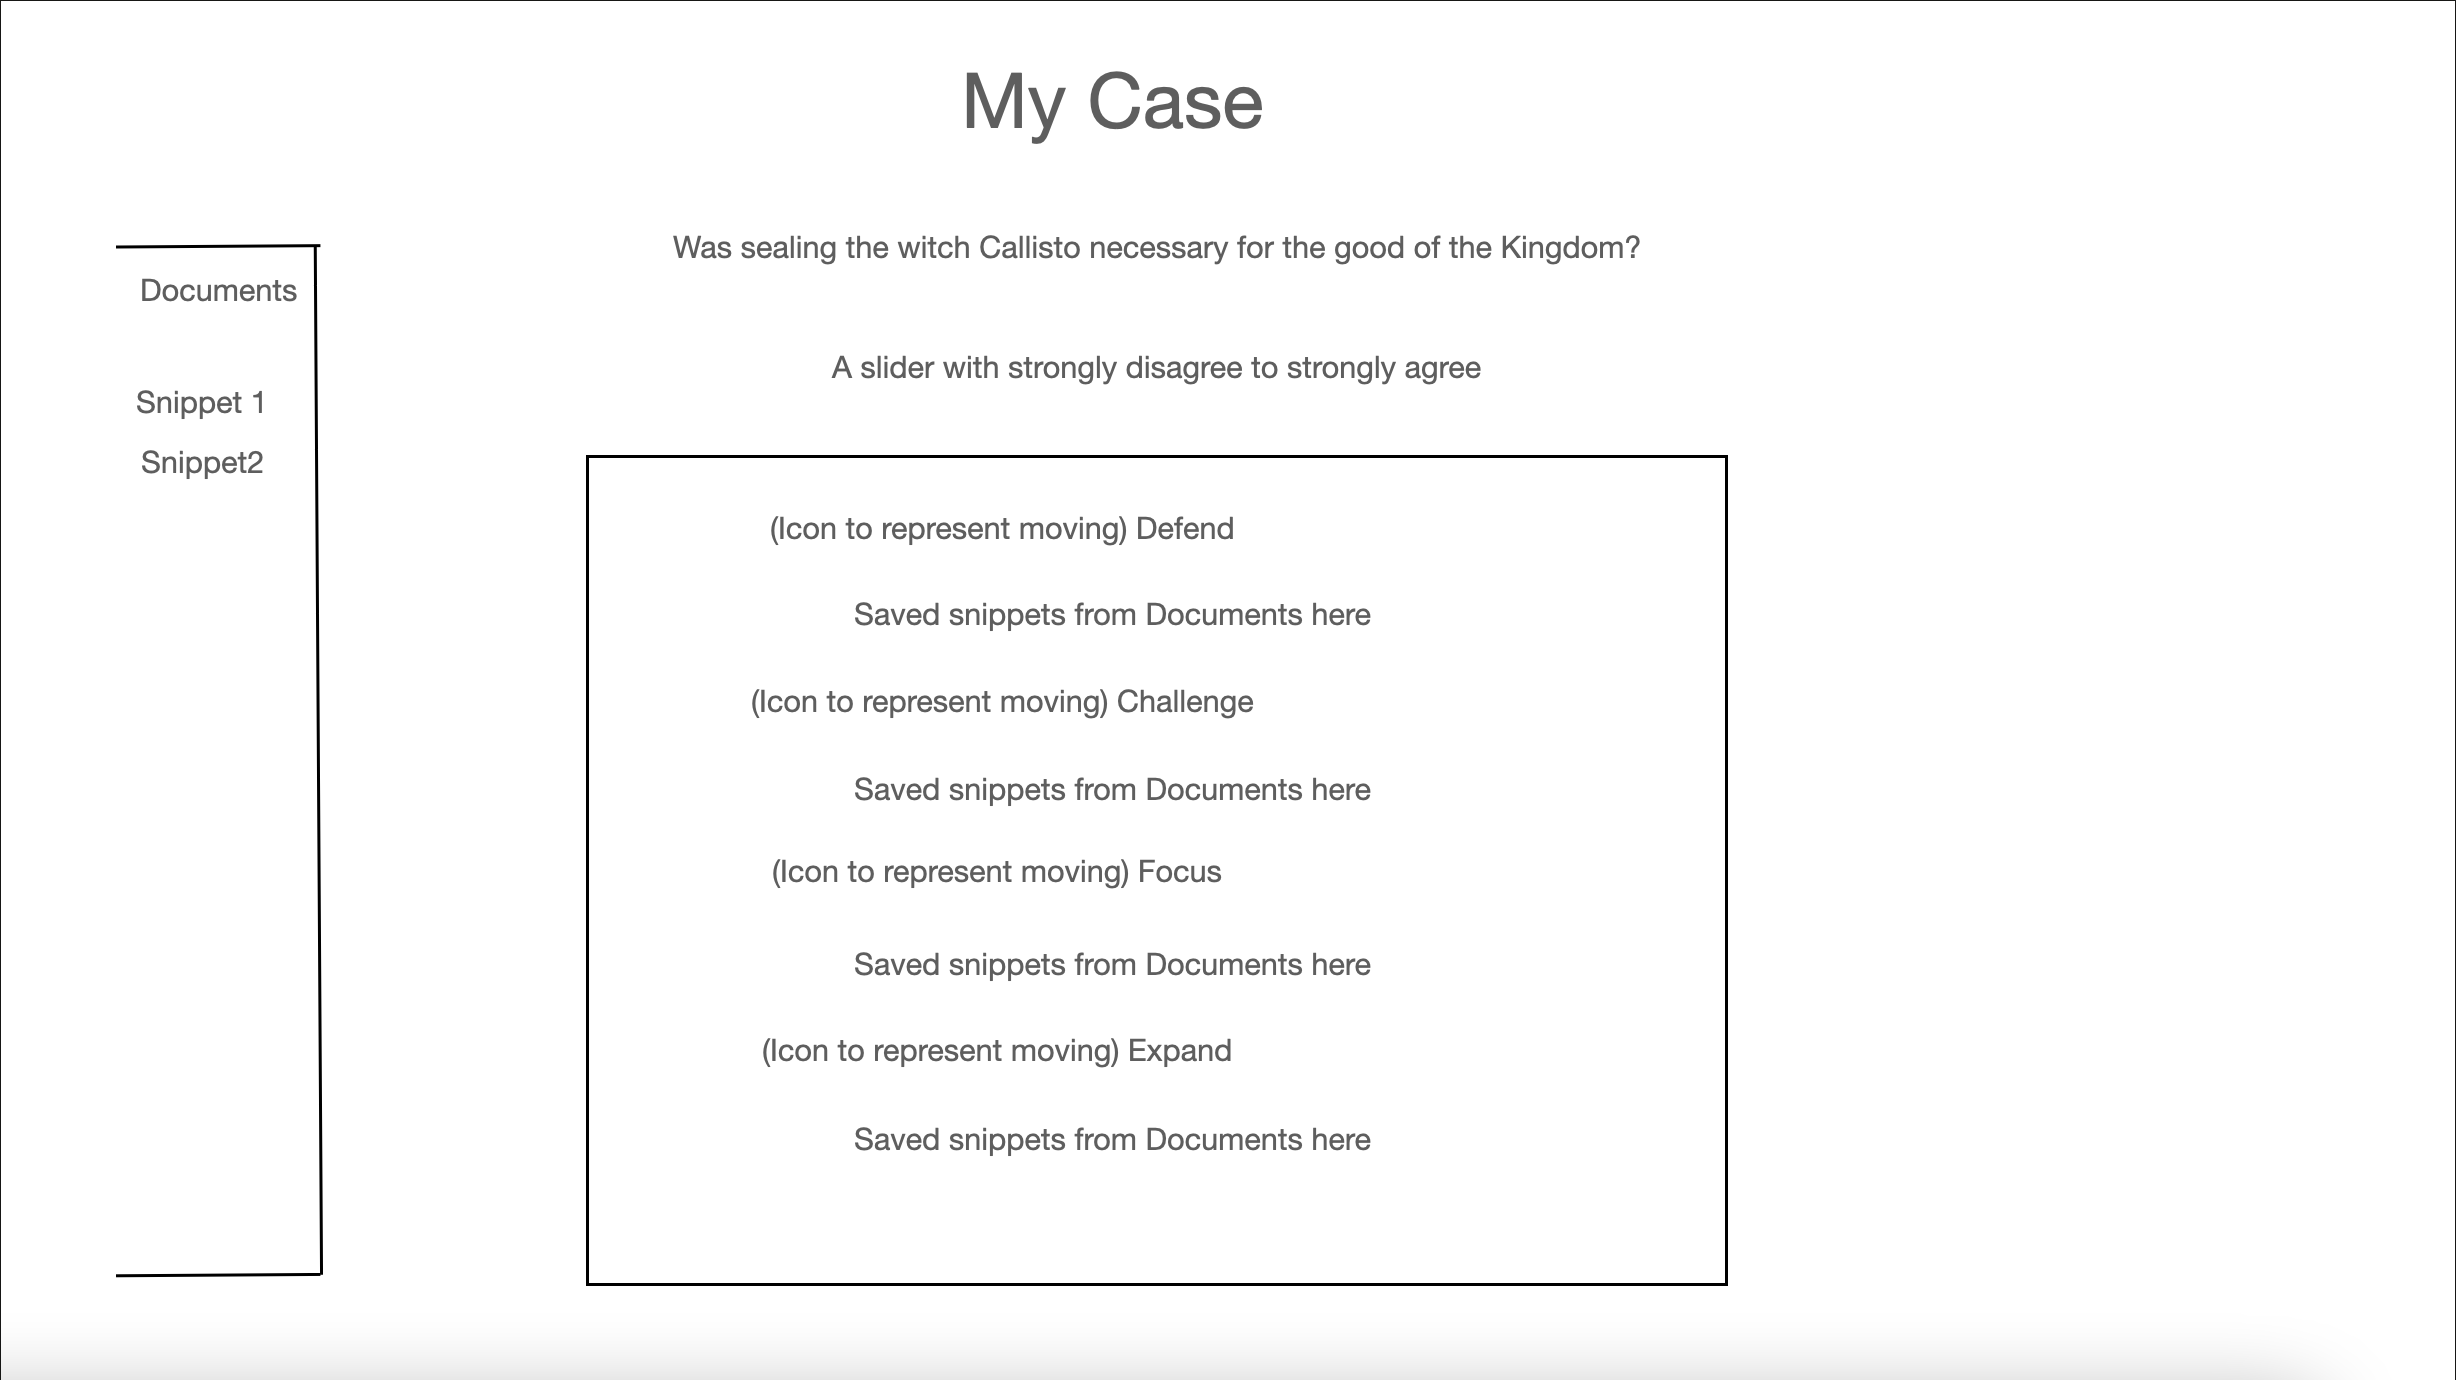
\includegraphics[scale=0.3]{images/MyCase_Paper.png}
    \caption{The Case screen of the Evenir Case Files game in its first, paper iteration.}
    \label{fig:Case_Paper}
\end{figure}

\section{Iteration 1 - Code Prototype}
\subsection{React Overview}

The previous sections outlined the content and presentation requirements of the game, and validated the concept through a paper prototype, but the question now turns to how best to implement those requirements from a technical standpoint. The robustness of this phase of development is crucial, because as the software development literature shows, a project not meeting its requirements is one of the principal reasons for its failures \citep{schwaber2002agile}, so it is worth discussing here.  The author of this research project chose to implement the software prototype in React, an open-source front end library for building user interfaces based on the JavaScript programming language \citep{react}. Before the decision was made, several other JavaScript-based frameworks were considered. One was Phaser, which is very popular for lightweight browser games \citep{phaser}. However, Phaser was rejected on account of its focus on graphics rendering. Because the library assumes users are dealing with graphics, the architecture it enforces would have required implementing additional rendering methods redundant to a text-based game. Another contender was Twine, a tool designed specifically to produce text-based games \citep{twine}. However, Twine is also principally designed for non-technical users, with its own graphical user interface, language and procedures. Although it can be supplemented with custom JavaScript, this is still limited by the need to go through Twine-specific features. React, on the other hand, offered the right balance of power and flexibility. It takes care of rendering elements, and allows for the easy reuse of graphical elements, which React calls “components”. React is also a well-supported and broadly documented framework because of its popularity, much more so than Phaser or Twine. This combination of features and support is what made the author decide on React for the technical implementation of the Evenir Case Files game. 

\subsection{Development Challenges - Architecture}

Having decided on what framework to use to develop the game, the next challenge was deciding what the appropriate software architecture should be. \citet{dawson2000twenty} notes that software architecture is an important phase in the Agile software development process, as changing customer requirements means that architectures should be left open and flexible to quickly respond to such changes. In the case of this research project, the concern was not so much of requirements changing, given that those were derived from literature and primary evidence, but that elements of the game would change as a result of the user evaluations, which the architecture needed to be flexible enough to accommodate. Figures \ref{fig:Architecture_1} and \ref{fig:Architecture_2} illustrate the component tree of the final version of the research product. This is a standard architecture for React projects because it is enforced by react-router, the library used in this project to route players through screens of the game, which are themselves components or a subtree of components. All the components created by the author of this project, such as Footer and MyCaseButton, are children of a Route component, and the BrowserRouter component provided by the react-router library is responsible for determining which Route to render along with its children. Figure \ref{fig:Architecture_2} is an example of how the place screens in the game are architected. This is also typical of a React project. Nesting components is the React way to keep individual code modules small and self-contained, which makes responding to changes faster in that isolated areas of the code can be altered or expanded upon without having to touch the rest of the project. This is a practice recommended by \citet{dawson2000twenty} and \citet{schwaber2002agile}. By relying on paradigms enforced or suggested by the React framework, the architecture chosen for this project is buttressed by software engineering best practices.

\hfill \break

\begin{figure}[!htb]
    \centering
    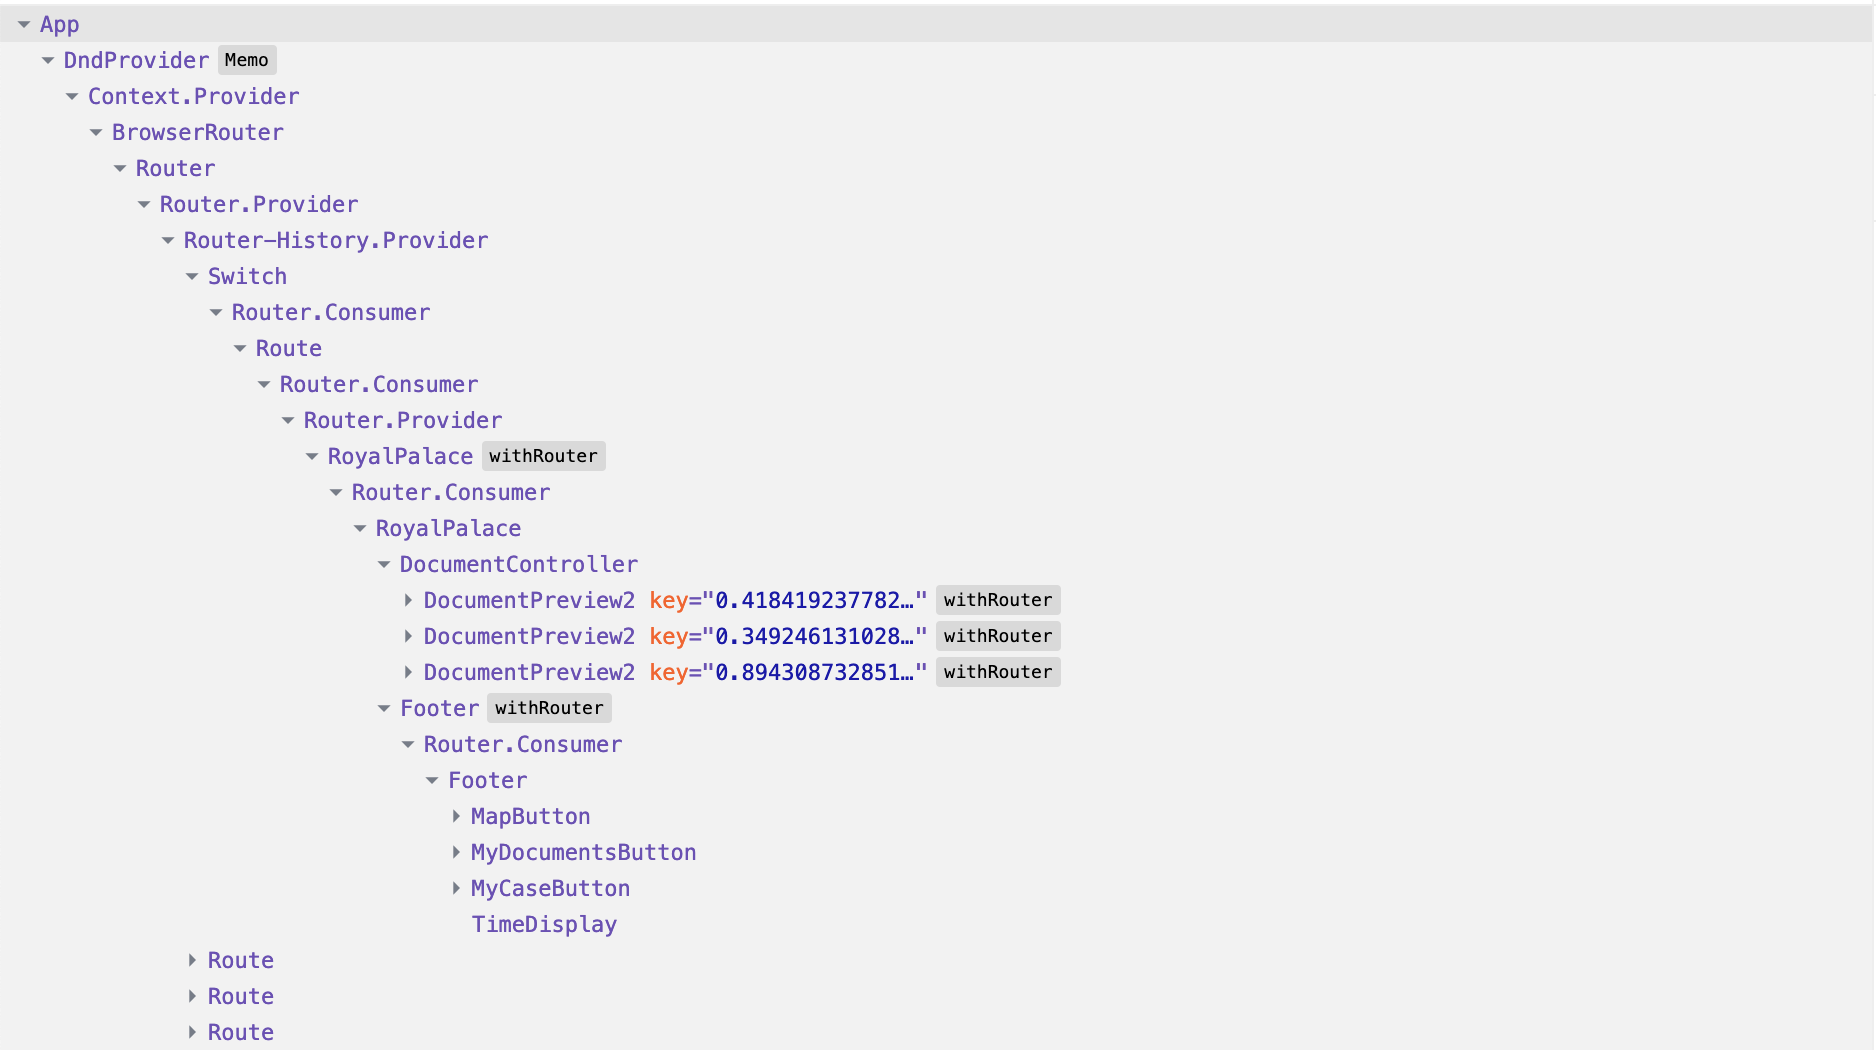
\includegraphics[scale=0.4]{images/Architecture_1.png}
    \caption{The component architecture of the Evenir Case Files game in its final iteration.}
    \label{fig:Architecture_1}
\end{figure}

\begin{figure}[!htb]
    \centering
    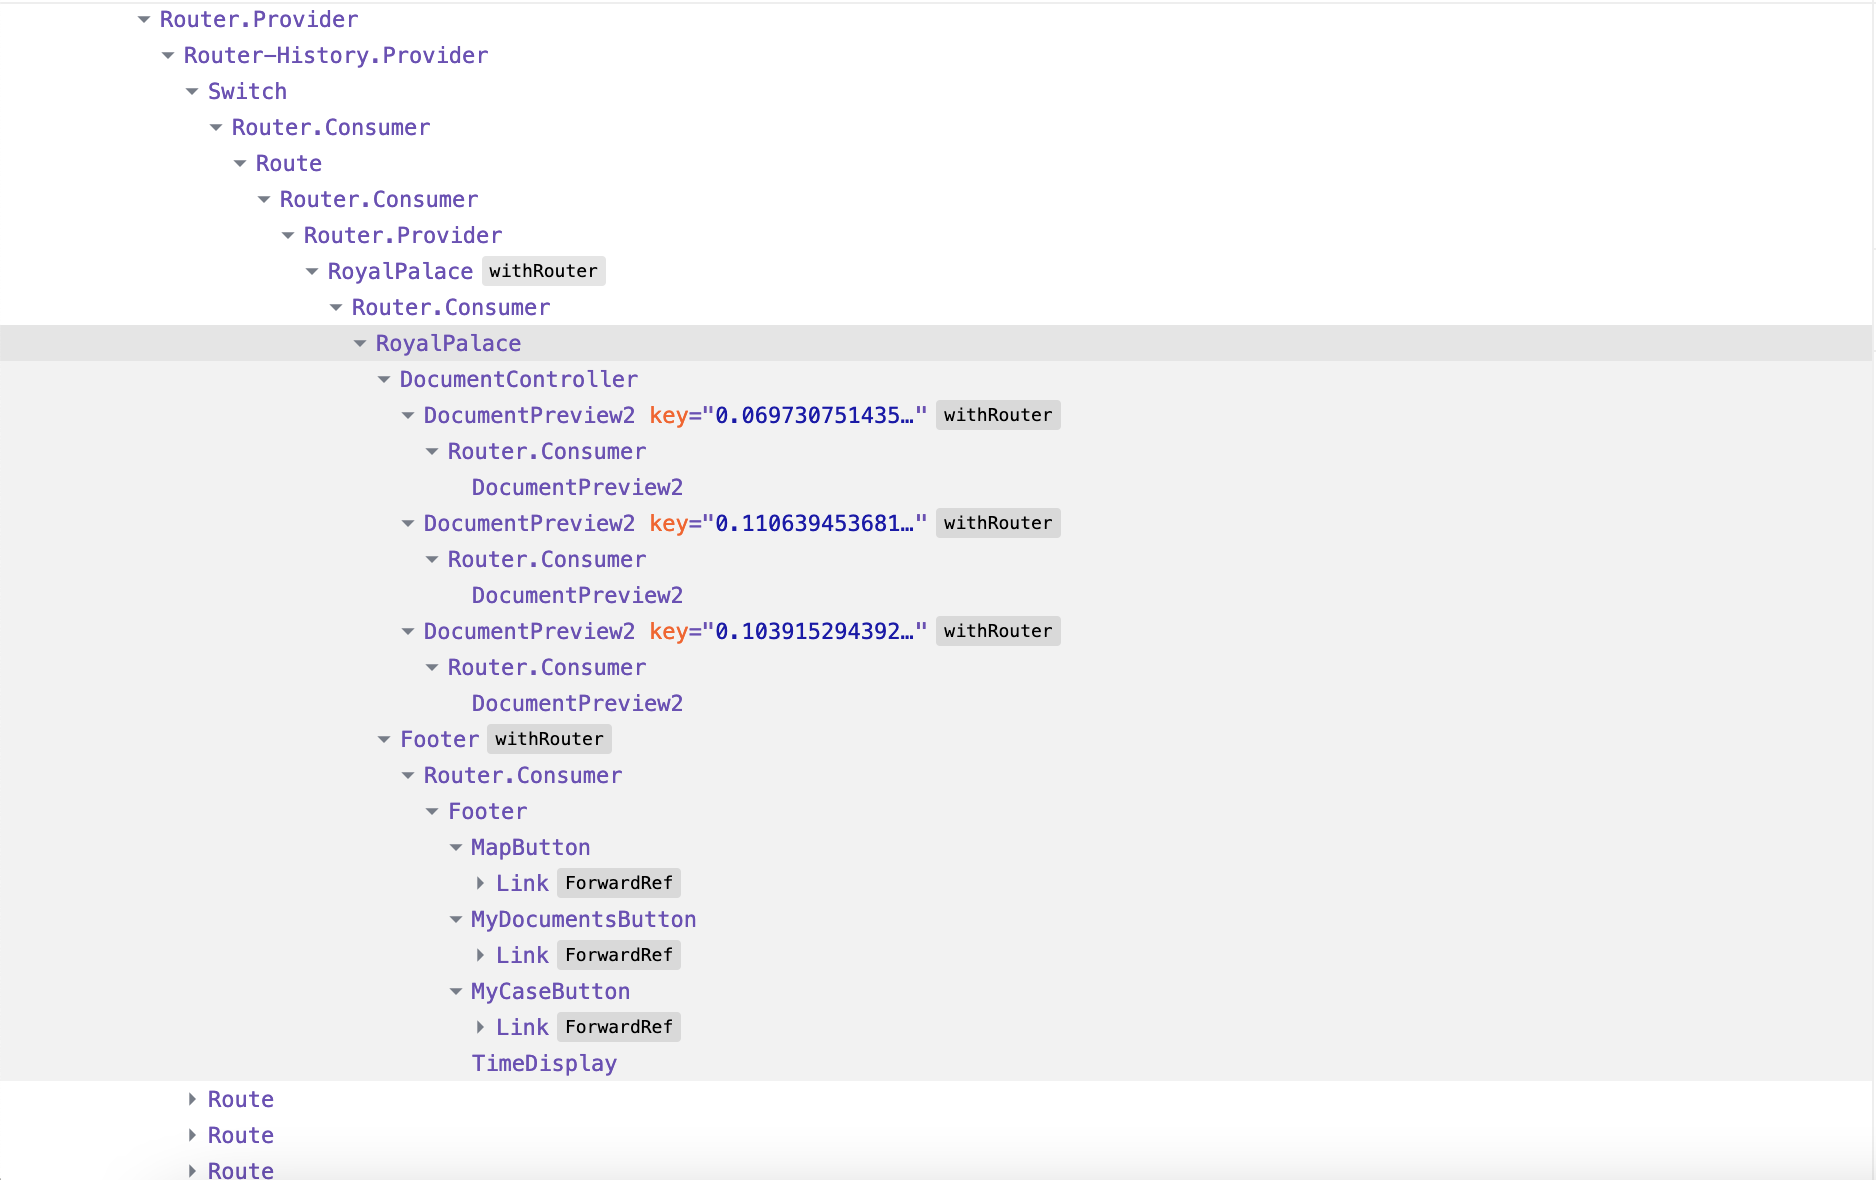
\includegraphics[scale=0.4]{images/Architecture_2.png}
    \caption{A detail of the component architecture of the Evenir Case Files game in its final iteration, to illustrate the Document component sub-tree.}
    \label{fig:Architecture_2}
\end{figure}

At an individual component level, the structure of the game evolved over time. Initially, a DocumentPreview component was responsible for rendering the title of one of the source documents of the game. Clicking on the component would trigger a modal popup which would display the text of the source document, which was handled through a stateful Document component. Each individual line of text was rendered by a DocumentText component. However, the Document component was also responsible for updating the timeline. This made it the longest class in the web app, at fifty-five lines of code. \citet{fowler2018refactoring} suggests that a long class is indicative of a software “smell”, an opportunity to improve the code. In this case, the author was violating the Single Responsibility Principle best practice outlined by \citet{martin2002principles}, which states that each class in a software project should be responsible for one thing only, to ensure the extensibility and maintainability of the code. The author thus followed the recommendation of \citet{fowler2018refactoring} and “refactored” the code, extracting the function to update the timeline into a separate scripts file. Furthermore, a separate file for the text strings of the source documents was created, and these were passed in as parameters to the Document class so that the content of a document could be easily updated without having to modify the Document code itself. These improvements to the codebase proved to be useful when the Document subtree component architecture was modified following the user experience evaluations detailed in the next sections. Actively looking for refactoring opportunities at a component level is another example of how development best practices were employed to ensure a high-quality research product. 

\subsection{Development Challenges - Data Flow}

Another challenge faced in the development of this research product was structuring the flow of data through the components of the game in a sensible way. This is a common difficulty in React projects, because of the nested architecture they tend to follow, as illustrated in the case of this game in Figure \ref{fig:Architecture_1}. The main example of this from the development of the Evenir Case Files was passing data from the Documents component to the TimeDisplay component, which is responsible for displaying how much time the player has left. In React, when two components are in a parent-child relationship, passing data is straightforward. The parent can pass data down to the child through React properties, or the child can pass data up by manipulating React state. When two components are siblings, data can be passed between them using their parent as an intermediary. However, as Figures \ref{fig:Architecture_1} and \ref{fig:Architecture_2} show, the Document component and TimeDisplay component are not in a direct parent-child or sibling relationship. Although all React components are children of the App component, placing data so high up in the component tree would have been rendered the data transfer itself cumbersome, on account of potentially having to pass data down many levels. Any change to the architecture as a result of user experience evaluations would have broken the flow of data and potentially required re-architecting the entire game. 

A common, though not necessarily simple, solution to this problem would have been to employ Redux. Redux is a React library which manages the entire state of the application with a single global object called Store \citep{redux}. The Redux Store allows component access to data to happen at any level of the tree, without requiring parents to pass it down via properties or state. That said, because Redux alters the architecture of React projects in a significant way, introducing Redux after architecture decisions have already been made is not an easy task. The author of this research project had to balance performance and scalability concerns with the speed at which a solution to the problem could be implemented in order to evaluate the game with real users. Following the advice of \citet{salen2004rules}, who recommend that at an early stage of game development, speed should be prioritised over other concerns, the author looked for an alternative solution. The final decision was to use the local storage of the browser as a sort of global store which could be accessed from any point in the component tree. Though this solution is not as scalable or efficient as Redux, and introduced infrequent performance bugs depending on the browser of the player, it allowed the author to hasten towards a point where testing the game with players was possible.  

\subsection{Styling the Game}

At this point in the development process, the functionality of the game prototype was complete, and the final step before user evaluations was to work on its visual presentation. \citet{isbister2010designing} make a compelling case for why presentation matters even in the early stages of a software prototype for a game. The authors survey experienced game design practitioners to ask what factors they consider important to design GBL experiences, and one of the recurring themes was “polish”, that there should be “no rough edges in appearance or interaction”. The reasoning for this goes back to the importance of fantasy as a motivational factor noted by \citet{malone1980makes}. The designers surveyed by \citet{isbister2010designing} note that this does not just apply to the content of the game, but its appearance as well, and neglecting appearance is a reason why many educational games fail to accomplish their objectives. To ensure that the appearance of the game met its research objectives, the author of this project was guided by the concept of external consistency, a usability principle popularised by NNG \citep{nng2021consistency}. External consistency suggests that a system can be made more intuitive if it does not differ too dramatically from what users expect to see in similar systems. For the Evenir Case Files, this meant that the author sought inspiration from similar games to determine what its appearance should be. Fortunately, considering the development costs that computer graphics can entail, fantasy text-based games appear to cherish plain, “old-school” aesthetics reminiscent of the early days of computer games. Figure \ref{fig:sryth} is an example screenshot from Sryth, one of the oldest but still most popular fantasy MUD (Multi-User Dungeon) games \citep{sryth}. The author of this research project decided to retain the “medieval” aesthetic through the beige colours and serif fonts which can be seen in Figure \ref{fig:case_final}, but otherwise opted for a more modern, minimal interface that is the contemporary trend in web applications. Thus, the appearance of the Evenir Case Files game, as well as the technical implementation, is grounded in the literature as well as best practices from industry.       

\begin{figure}[htb]
    \centering
    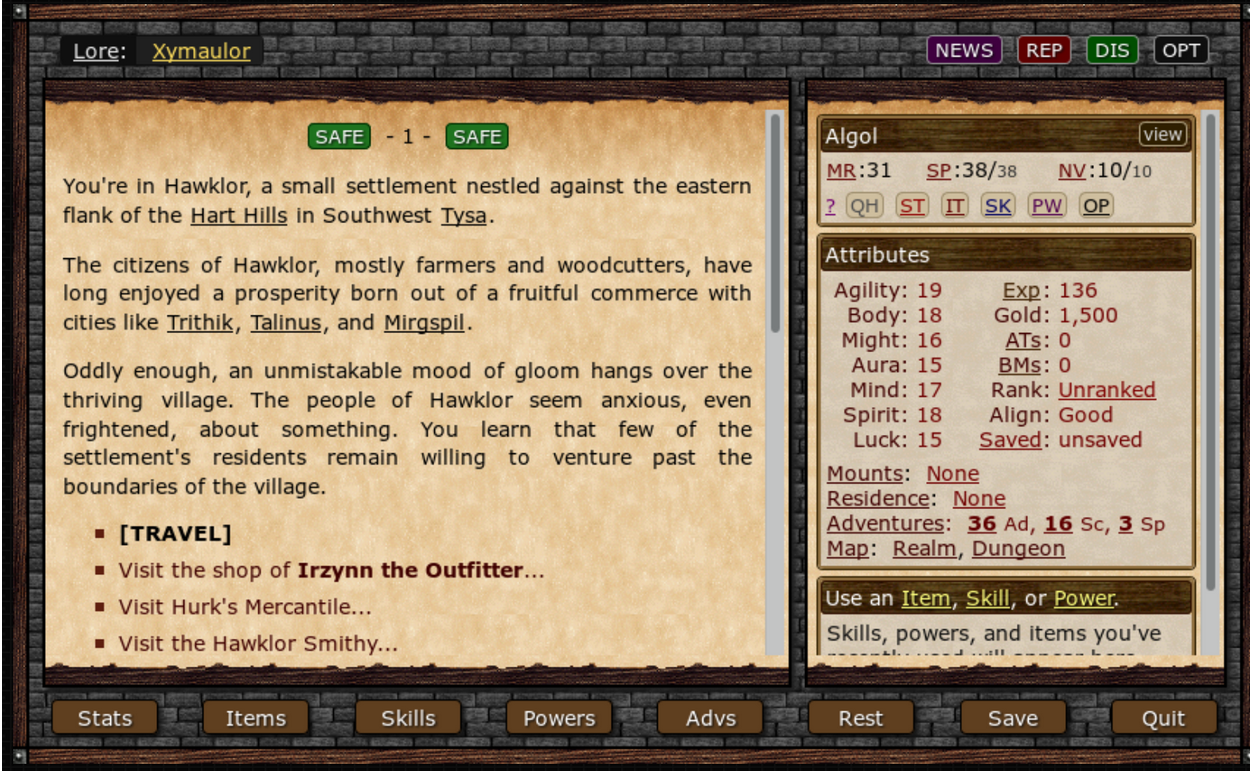
\includegraphics[scale=0.5]{images/SrythScreen.png}
    \caption{A representative page of the MUD game Sryth. The author of this research project used games like Sryth as a guide to design the Evenir Case Files, based on the principle of external consistency.}
    \label{fig:sryth}
\end{figure}

\section{Iteration 2 - User Experience Improvements}

This iteration was the first set of think-aloud evaluations the author of this research project ran to improve the game. At this stage, two evaluations were conducted, which yielded both reassurance that certain aspects of the game were strong and suggested directions for improvement. Both participants noted that the story was the strongest aspect of the game. One said it was “quite compelling”, reminding them of the popular Witcher franchise, and also pointed out the appeal of the colour scheme selected by stating it reminded them of “an old book page”. When asked if they would play the game again, the participant replied that they would play to find out more about the story and the characters the player was asked to investigate. The second participant went a step further in appreciating the setting of the game by stating that they enjoyed the fact they were dealing with “chronological lore” in the game, because they found it “an interesting representation of how a historian would do their job”. They later stated they would continue to play the game only if it were explicitly presented to them as a game which allowed them to play the part of a historian, as they felt that was its most unique appeal. These first comments were promising evidence that the work the author had put into developing a detailed fictional setting and making sure the presentation matched it, as suggested by the literature, was well-motivated. 

There was also consistency in the areas of improvement to be addressed before the game could be considered complete. Both participants noted that they did not realise certain key features were present in the game. The first was the fact that the text anchors which linked one page of the game to another, as well as revealing historical documents, were clickable. One participant noted that the fact that the anchors were in a bulleted list did not imply clickability to them, and they only realised that was what they had to do because they had clicked everything else on the screen. The other participant noted that their mouse cursor did not change on hovering over the anchors, which also suggested that those anchors were no different from regular text. The second feature the participants had difficulty with was the fact that individual sentences in documents could be dragged into the sections of the Case page. One participant stated they did not realise they had to click on the text before being able to drag, and that they did not realise they could drag individual sentences. The other participant tried to drag entire documents into the Case page sections, and expressed confusion when that did nothing. In both cases, the author had to directly point out that individual sentences could be dragged. The third issue was with the slider that players need to drag to state how strongly they agree or disagree with the question they are asked to investigate. Both participants did not realise the slider locked into place and needed to be dragged past a certain threshold to move to adjacent markers. The participants also expressed difficulty understanding what the sections in the Case page meant, however, the author decided to prioritise the first set of problems for this iteration, since as opposed to being an issue local to the Case page, difficulty understanding how to navigate through the game had a serious impact on the entire play experience. 
The underlying problem in these issues, the discoverability of features, is a well-known one in design literature. Don Norman, one of the founders of NNG, popularised the term “affordances” to describe characteristics objects have which give clues as to their behaviour. Door handles, in Norman’s famous example, afford pulling, but if that door is instead a push door, there is an affordance mismatch \citep{norman1988psychology}. Since then, NNG have written extensively about affordances, including specifically how to suggest clickability in contemporary “flat” design web applications which were one of the inspirations for the Evenir Case Files \citep{nng2015links}. Their key recommendation is to make sure links stand out in the web app and to make sure that links are presented consistently throughout. This is based on the usability heuristic of internal consistency, the complement to external consistency which guided the aesthetic decisions outlined in the previous section \citep{nng2021consistency}. Of course, a mouse cursor not changing over a link on hover also broke the principle of external consistency in software more broadly, as that is the expected behaviour of links \citep{nng2021consistency}. As a result, the author of this research project sought to denote all interactive elements in the game with their own blue colour, which would stand out from the non-interactive elements. This meant the “next” button in the first pages of the game, the text anchors which linked pages together, document titles, which were also modified to have the cursor change when hovered over them, as well as the slider in the Case page. Furthermore, individual sentences in documents were modified so that they would be underlined in the same blue colour when hovered over in the Case page. Figures \ref{fig:Map1} and \ref{fig:Map2} illustrate certain pages of the game before and after the changes made. This raft of user experience improvements were implemented to address the key issue of discoverability highlighted by both participants in the first round evaluation.

\begin{figure}[htb]
    \centering
    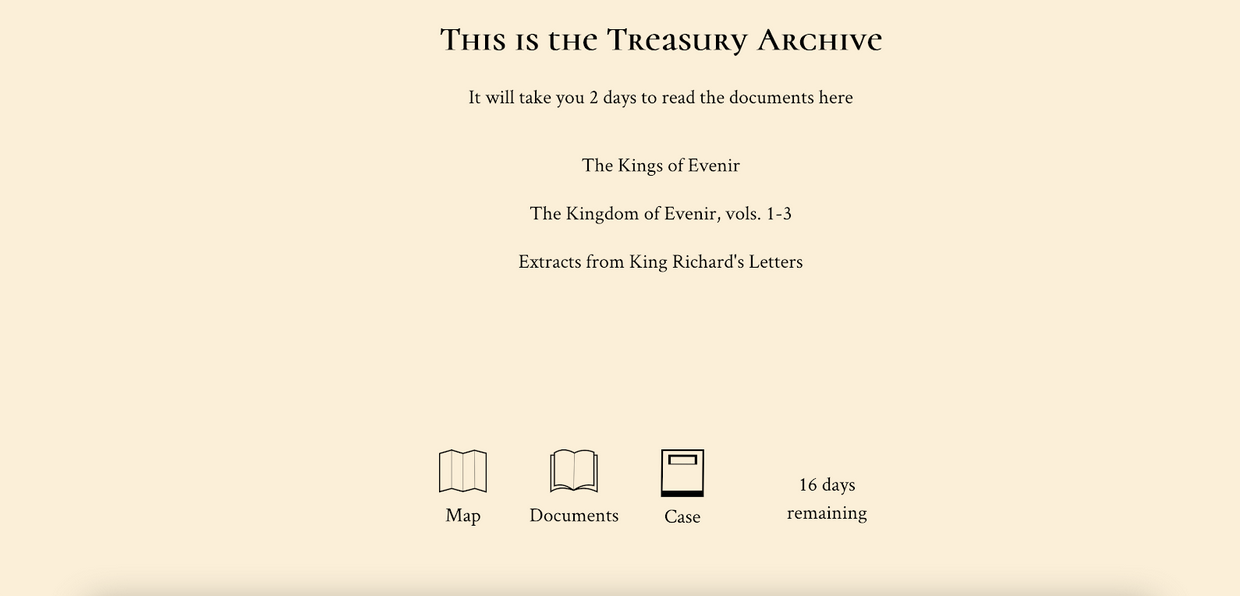
\includegraphics[scale=0.55]{images/Map_1.png}
    \caption{The Map page of the game at the beginning of this iteration. There is no styling to differentiate clickable elements from non-clickable elements.}
    \label{fig:Map1}
\end{figure}

\begin{figure}[htb]
    \centering
    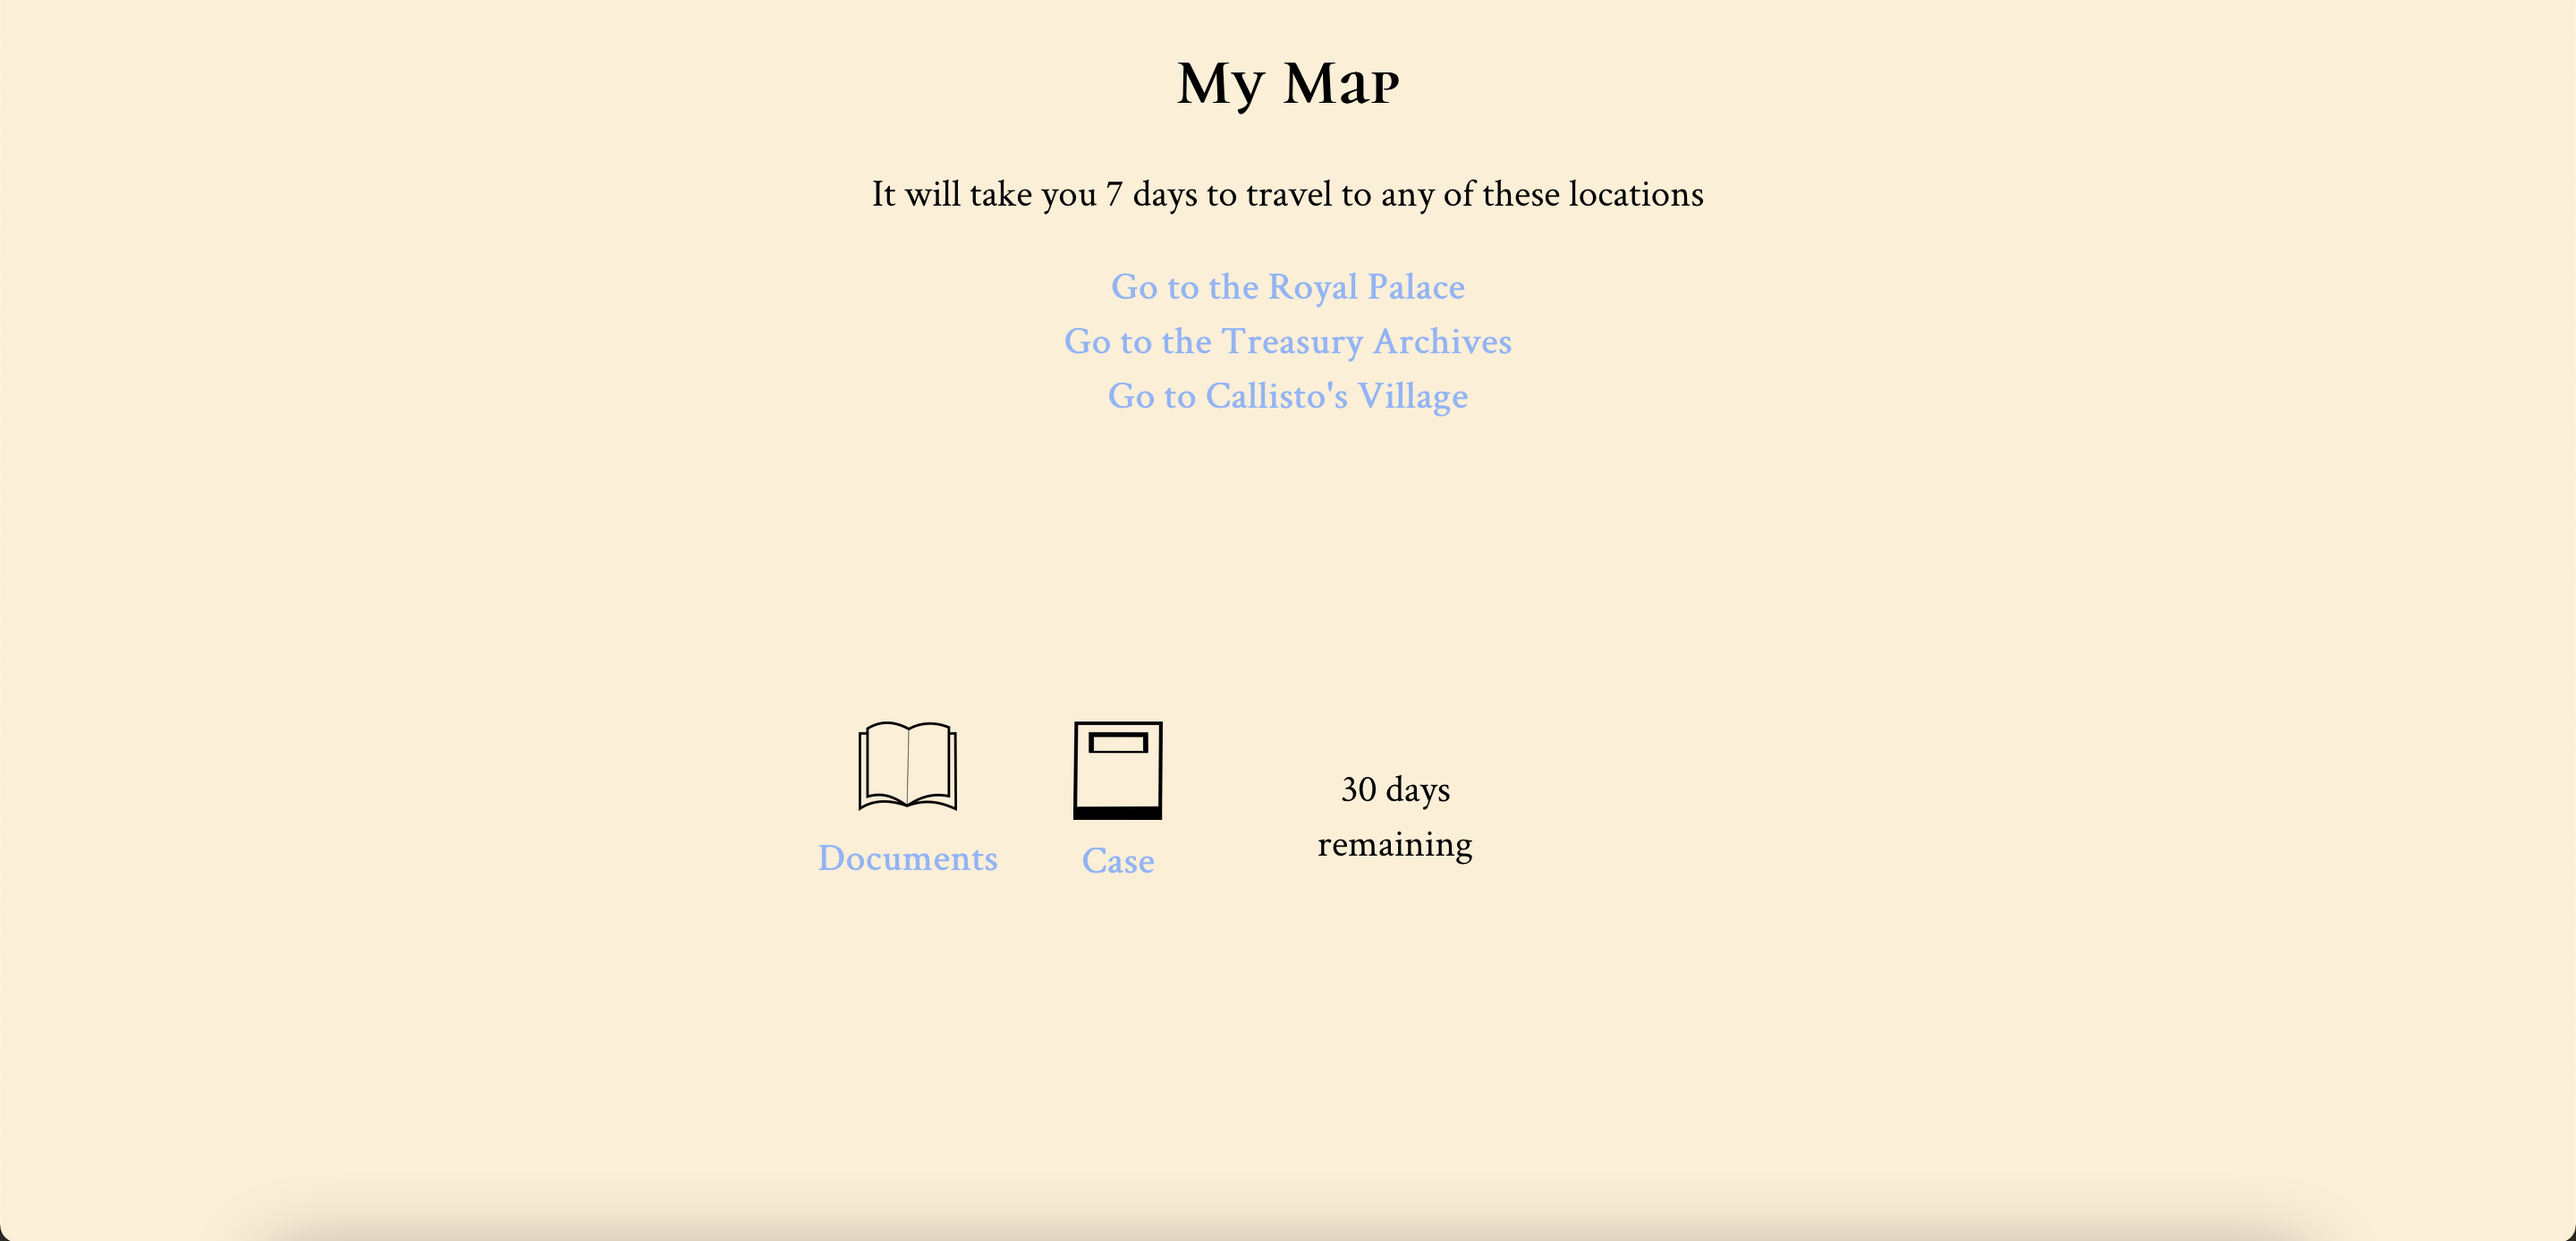
\includegraphics[scale=0.25]{images/Map_2.png}
    \caption{The Map page of the game at the end of this iteration. All interactive elements have been clearly and consistently highlighted in blue.}
    \label{fig:Map2}
\end{figure}


\section{Iteration 3 - User Experience Improvements, Continued}

Three new participants evaluated the game at this stage. There was, again, consistency in the remarks on what the game was doing well and on areas for improvement. Two of the three participants noted that the story was the element of the game which drew them in most, with one specifically noting that the presentation of characters with conflicting motives is what drew them in to want to find out more as they were reading. The other noted that they found leaning more about the world and the story as they read documents an appealing mechanic. This sentiment was echoed by the third participant, who stated that was the element which they found most appealing. Crucially, at this stage, all three of the participants did not appear to have significant issues navigating through the game or interacting with the Case page. There was no hesitation as they clicked the now blue text anchors, and the fact they needed to drag document sentences into the case sections was clear to them as soon as they hovered over one of them. The slider being blue also meant that the players did not hesitate in clicking and then dragging it. Although the lock meant that they did not receive immediate feedback when dragging, the fact that it was the same colour as the links reassured them that this was an element it was possible to interact with, so unlike in the previous iteration, they continued to drag until it moved past the threshold. When asked about the controls of the game directly, all three participants stated that with the exception of the Case page sections, all the controls felt intuitive or that the game was easy to navigate. This confirmed the course of action outlined in the design literature the author used to solve the problem of discoverability. 

The first issue with the prototype at this stage concerned the presentation of documents. These had been designed as pop-up modals using cascading style sheets (CSS), but resizing them to adapt to different screen sizes proved to be an unexpected challenge as a consequence, since CSS requires the positioning of elements relative to each other to be explicitly stated and effects can vary based on specific browsers. One of the participants pointed out that the documents were covering the Footer component, which was very aesthetically jarring. Another participant pointed out that the way the documents were appearing on the page right now, they did not make sufficiently clear that reading documents subtracted from the remaining in-game time of the player. This meant that the strategy the participant had tried to adopt to meet the objective of the game was derailed, which they noted dampened their enjoyment of the game by a significant amount. Considering the importance of polish and the timeline mechanic outlined in the previous sections, the author decided to prioritise addressing this issue. This was done by implementing “pop-up” functionality using React state as opposed to CSS, to ensure precision in the layout regardless of browser peculiarities, as the documents were now positioned by the markup rendered internally by React and not modified with additional CSS specified on top of it. Doing so required restructuring the architecture of the Document component sub-tree. A new DocumentController component was created, which was responsible for deciding whether to display DocumentPreview components or individual Documents, depending on what the player had clicked. The ability to quickly make an architecture change at a late stage of prototype development was in large part due to the refactorings described in the Architecture section of this chapter, since each component in the Document subtree was relatively independent of the other. The result of this change was that clicking on a Document now appeared to “push down” the Footer component, and therefore the TimeDisplay, on the screen, and closing it brought it “back up”. This change in positioning was done to highlight the fact that clicking on documents cost in-game time, thereby addressing the issue noted in this iteration. 

\begin{figure}[!htb]
    \centering
    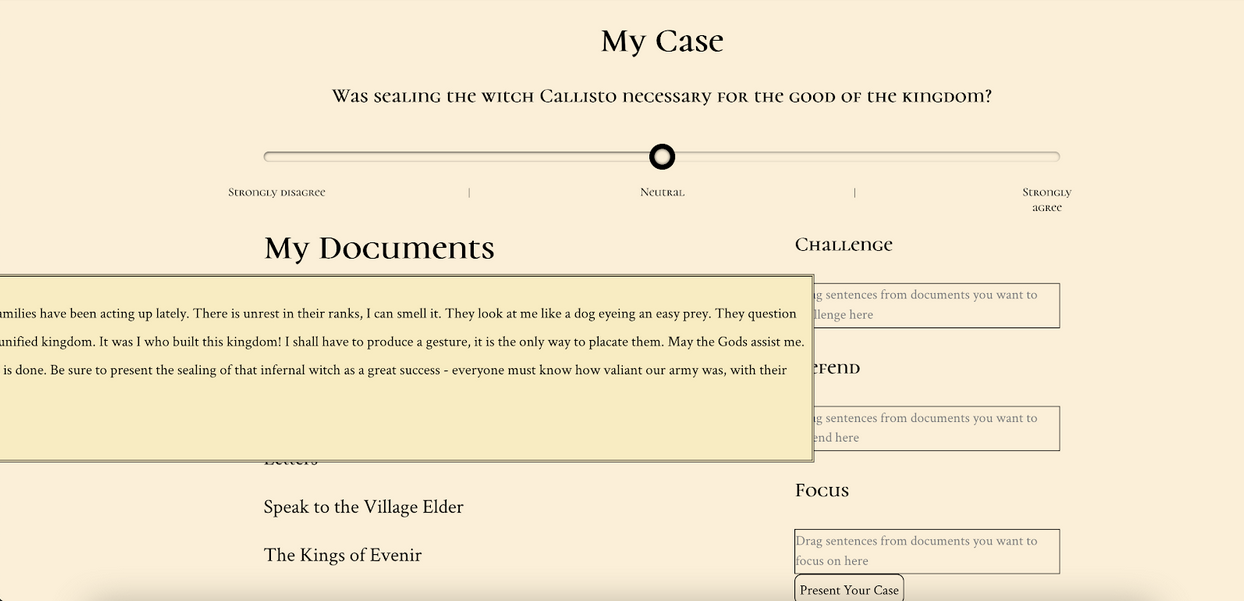
\includegraphics[scale=0.6]{images/MyCase_1.png}
    \caption{The documents in the Case page as they appeared at the beginning of this iteration. Note the overflow caused by the "pop-up" functionality being implemented in CSS, and the lack of text highlighting.}
    \label{fig:Case1}
\end{figure}

\begin{figure}[!htb]
    \centering
    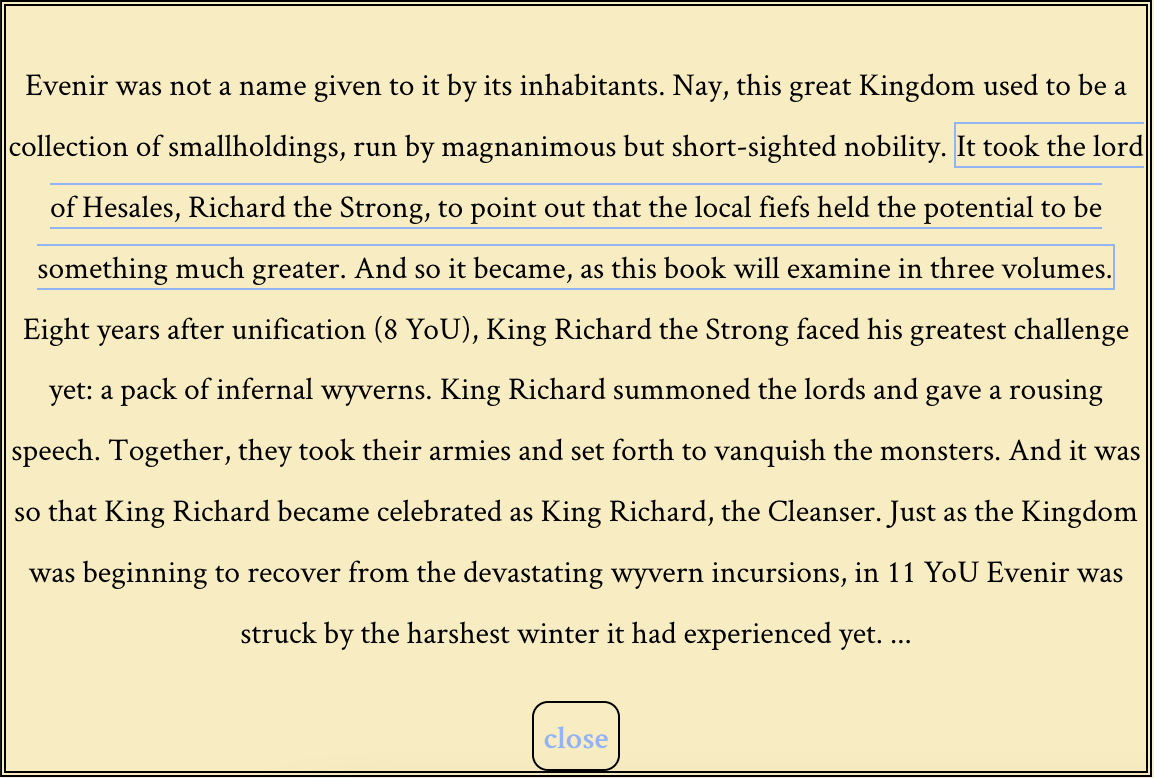
\includegraphics[scale=0.6]{images/MyCase_2.png}
    \caption{A detail of a document in the Case page at the end of this iteration. Note the text highlighting.}
    \label{fig:Case2}
\end{figure}

The second issue the author of this research project tried to address was the confusion caused by the Case page sections. Most participants in all previous rounds expressed confusion at whether the sections, initially named “Challenge”, “Defend” and “Focus” referred to the sentences themselves, or the relationship between the sentence and their relevance to the question they were asked to investigate. There was also confusion expressed as to what the section titles themselves meant. To address this, the author first renamed the “Focus” section to “Emphasize”, since that was the one which participants most consistently expressed confusion over. Placeholder text was also added within the sections themselves, to reinforce the idea that the sections were intended to challenge sentences placed within them. A title was added above the case sections to reinforce the objective and the fact that it was not mandatory to add in sentences in all the sections. 

\section{The Final Research Product}

The Evenir Case Files game was developed to be a tool drawing on a strong research background to ensure it would best capture the objectives of this project. The content and presentation of the game was informed by the research goals of this project, GBL literature in \citet{malone1980makes}, and two key game design texts from \citet{fullerton2004game} and \citet{salen2004rules}. The game itself was developed with a focus on best practices from the Agile software development literature, using modern frameworks and libraries in React and with an emphasis on iteration and incremental improvements to the codebase as espoused by \citet{schwaber2002agile}. Finally, this research focus was also accompanied by evaluations with real users, according to best practices in design literature along the lines proposed by \citet{gulliksen2003key}. These user evaluations, combined with an Agile approach to software development, meant that the details of how the game was implemented closely reflected the requirements set by the literature. 

At this stage, the game was evaluated with one think-aloud evaluation and five remote evaluations, at the end of which the authors compiled the \citet{fullerton2004game} survey in written form. This hybrid approach was designed to elicit some in-depth feedback at this stage while also checking that the game’s user interface and experience was robust enough that it could be played without the author being present in case things went wrong. The feedback was mostly positive. The five remote participants all expressed a clear understanding of the objective of the game, ranging from “travel around to do research and produce a compelling argument” to more nuanced answers like “gather information surrounding the history of the kingdom and the events surrounding the events of Callisto and then analyzing said information to find contradictions in the story to potentially prove the innocent or guilt of the witch”. All respondents also stated that they had no issues with the controls of the game and that the information they needed was easy to find. Half the participants, however, did note they had some issues still with assembling their case. From the one think-aloud evaluation the author conducted at this stage, the participant was able to understand the relation between the case argument and the sections, but was not fully clear on what the sections meant. The author also followed up two of the remote evaluations with additional clarification questions, and those participants stated that they were not initially clear on this relationship, but they eventually understood. This was also stated by the remote participants the author did not follow up with. Thus, although it appears that in the final instance of the research product there was still some confusion with the user experience of the Case page, this was an improvement over the total confusion in the previous iterations. Combined with the confidence the remote participants expressed in describing the objective of the game and the controls, the author felt that it was reasonable at this point to move onto the final study design and evaluation. 

\chapter{The Final Evaluation}
\section{Virtual Worlds – Study Design}
One of the oldest and most widely employed tools to measure CT skills is the Watson-Glaser Critical Thinking Appraisal (WGCTA) \citep{bernard2008exploring}. The WGCTA is structured as a multi-part written test posing questions with a single correct answer, measuring five different components of CT \citep{bernard2008exploring}. The WGCTA was most widely administered in the United States in nursing programs, given the increasing importance placed on CT skills in those curricula \citep{bauwens1987use}. The typical study design there employed is a pre and post-test design where participants take the WGCTA before beginning their program of studies, and then agree to share their final grades upon completion of the program, or sit the test again. Although the WGCTA has generally shown to be reliable under some statistical aspects \citep{bernard2008exploring, bauwens1987use, crouch2015predicting, el2007validating}, authors including \citet{crouch2015predicting} and \citet{el2007validating} find that it can struggle to act as a predictor of the ability to think critically in the future. \citet{el2007validating} suggest this may be due to factors such as the difficulty with transferring CT skills from one domain to another, a lack of student motivation to apply CT, and the absence of university programs explicitly designed to engage student CT skills. This would be consistent with the argument developed in Section 1.1 of this research project, which raised the importance of domain-specificity and CT dispositions. Because of the focus of this project on the specific domain of history, and the inability to conduct test participants over a long instructional period, a study design based around the WGCTA was deemed inappropriate here. 

\citet{gelerstein2016designing} show that it is possible to develop an ad hoc instrument to measure CT skills based on the specific circumstances of the study. They develop a graphic novel targeting primary school children which adapts a popular story, and intersperse it with questions to elicit critical thought from their study participants. They validate their instrument through a variety of methods, including think-aloud evaluations and statistical tests such as Cronbach’s alpha \citep{gelerstein2016designing}. However, their model of CT is similar to that which underlies the WGCTA, conceptualising it as a combination of higher-order general-purpose cognitive skills like deduction and reasoning. As a result, the instrument has similar limitations to study designs based around the WGCTA when it comes to the problems of domain specificity and CT dispositions. Thus, although \citet{gelerstein2016designing} offer a useful precedent in the literature, the specific tool they develop is aimed at a different context and reproducing their methodology would not have been the most effective way to capture the objectives this research project.   

The model at the core of this research project is the Reflective Practitioner conceptualisation put forth by \citet{schon1984reflective} and outlined in Section 1.3, so the author sought to design a study which would reflect it appropriately. Crucial to this was the notion of “virtual worlds”. Schon defines virtual worlds as “contexts for experiment within which practitioners can suspend or control some of the everyday impediments to rigorous reflection-in-action” \citep{schon1984reflective}. For example, an architect models the plan of a building on paper to control factors such as the logistics of transporting materials, the specific characteristics of the terrain on which the building is being built, and so forth. This allows the practitioner to focus only on certain parts of the unique problem they face, which facilitates their ability to “see-as”, since it is easier to recognise a problem with fewer variables as something similar to an experience they have already had. Because “seeing-as” is the prerequisite for “doing-as” in the Reflective Practitioner model, a well-constructed virtual world is a fundamental problem-solving tool in the arsenal of the practitioner, and therefore to this study. 

The author of this research project developed the Evenir Case Files game as a virtual world for the historian, in that it excludes certain parts of the process of the historian outlined by \citet{tosh2006pursuit} in Section 1.2 from the gameplay. The process of external criticism, checking for the authenticity of the sources, is not part of the gameplay. Also excluded is assembling the sources into a coherent written argument, which is reduced to the drag and drop interface detailed in Chapter 2. Instead, the game is entirely focussed on the process of internal criticism of historical sources. The ultimate aim of developing a high-quality research product was thus to ensure the creation of a virtual world that faithfully mirrored this part of the process of the historian in an engaging way. Chapter 2 argues that the Evenir Case Files is such a virtual world, by virtue of the strong ties between the content and presentation of the game with the relevant literature. Consequently, according to the Reflective Practitioner model, all that was necessary to complete this study design was to identify a way to check that the game was indeed encouraging its players to “think historically”, as outlined by \citet{willingham2008critical} in Section 1.1.

Based on the precedent of an effective ad-hoc instrument offered by \citet{gelerstein2016designing}, the author of this research project designed a questionnaire that asked the participants to reflect on what they were doing as they were playing the Evenir Case File game and why they took certain actions. It was administered in the form of a semi-structured interview right after the participant played through the game. Because of the difficulty of conducting in-person studies imposed by the pandemic, the evaluations were conducted over the videoconferencing platform Zoom. Full transcripts of the study can be found in the Appendix, anonymised to protect participant privacy and manually edited to correct errors with the automatic transcription software provided by Zoom. A total of nine participants took part in this study. They were a convenience sample of students and recent graduates the author knew well, most in their fourth year of Computing Science at the University of Glasgow. The participants were selected on the basis that they had not taken any university-level history courses prior to the study being conducted. This was done to limit the confounding effect that previous experience in subjecting historical sources to internal criticism would have had on the results. For the same reason, none of the participants had seen or played through the Evenir Case Files game before. The questions are based on the process outlined by \citet{tosh2006pursuit} in Section 1.2, and are reproduced below. 
\begin{itemize}
    \item What was the objective of the game? 
    \item How did you go about completing the objective?
    \item Why did you put those specific sentences into those specific sections?
    \begin{itemize}
        \item why do you think the sentences you put in the ‘emphasize’ section were particularly important to your argument?
    \end{itemize}
    \item Why did you exclude the other sources from your case presentation?
    \item What do you think of the reliability of your sources?
    \item Do you think you had enough information to make a convincing argument? If not, what kind of information might you have wanted?
\end{itemize}

\section{Evaluation Results and Discussion}

The approach the author of this research project used to analyse the results was along the lines of the grounded theory methodology detailed in \citet{charmaz2007grounded}. First, for each question, all nine responses were grouped together and viewed side-by-side. This allowed the author to have an initial overview of similarities across participants. Then, categories were identified, broader themes which emerged from analysing responses across questions. This shortened form of grounded theory analysis is referred to as “affinity diagramming” in industry, and was selected because it is the qualitative analysis technique best suited to quickly identifying themes in the data \citep{NNGthematic}. The remainder of this section will go into detail on the principal categories the author identified through their analysis and how they relate to the research objectives set at the beginning of this report, presented in narrative form as recommended by \citet{charmaz2007grounded}. The subsections will first discuss the evidence that the Evenir Case Files game enabled players to demonstrate important CT skills in history, and then evidence for CT dispositions, one of the key differentiators of this project. 

\subsection{Critically Assessing Bias}

One of the key skills a historian must employ is dealing with bias in their sources \citep{tosh2006pursuit}. This relates to the skills component of CT such as analysis and evaluation, as described in Chapter 1. Assessing the bias of the sources participants encountered in the game is one of the first emergent themes worth discussing here. All participants who encountered the Royal Palace location stated that the sources there were biased in some way. On the personal letters of King Richard, P1 stated “you have to take [them] with a bit of a pinch of salt, because they’d obviously be subjective in nature (…) in his mind he’s the good guy.” On the official court histories, P2 noted that they were likely “ (…) pre-written books, extremely edited (…)”, while P3 stated they believed them to be “propaganda”. Considering the purpose a text was written for is the first step to critical analysis in history (Tosh and Lang). However, some participants took that acknowledgment of the likely bias of those sources one step further. On the letters of the king, P5 noted that they “wouldn’t, like, exclude [documents produced by King Richard or his government] from an investigation, but I think they would certainly be biased if they were written by him.” On the official court histories, P3 noted that they would have considered them a useful source if they could have found a document on the context or reason for which they were produced. The idea that a heavily biased source can still be useful to a historical argument is something which \citet{tosh2006pursuit} also note, and the fact that some players, albeit a minority, voiced such an opinion after playing the game is evidence that has the potential to encourage advanced levels of historical thought.

All participants who encountered the Village Elder character stated that they considered their testimony to be more reliable than the documents in the Royal Palace location. The two reasons given is that a character like the Elder would have been “closer to” the event the player was investigating, and that the Elder would not have “anything to gain” from manipulating the truth. Indeed, when asked about what other sources they would have liked to see, some participants stated they would have liked to hear from other similar figures, such as other villagers or knights in the employ of the king. The first intuition of closeness to the event under examination is supported by \citet{tosh2006pursuit}, who note that the historian will often prefer a source as close as possible to the events. The second point on having something to gain by portraying events a certain way inadvertently echoes a long-standing debate in the literature on the nature of historical truth \citep{carr2018history}. Both the points are further evidence of historical thought being encouraged. Here too there is evidence for the potential of sophisticated levels of thought being possible. P7 stated that to be convinced by the testimony of the Elder character, they would have liked to know something about their personality, and they also doubted the reliability of the memory of a person. As in the previous paragraph on the bias of official sources, the importance of personality and memory when dealing with sources close to events is also raised by \citet{tosh2006pursuit}. 

Most participants who encountered the statistical type documents in the Treasury Archives location considered them to be reliable. P4 stated that unlike the other documents, which were “rumours or hearsay”, the statistical reports were the only ones which could be verified by counting, and therefore the most reliable. P8 said that they believed numbers could be faked, but they could not imagine why this would have been done in the game. P3 was the only participant who strongly doubted the reliability of the documents in the Treasury Archives, noting that the documents were likely not “independently sourced right, it came from the same government that benefits from those numbers looking good, so it makes sense that they'd want to use it.” P1 made the interesting remark that “the treasury reports tell you, you, know the, the, effect on the economy, so obviously people were suffering, but you know you’re not really seeing the story being told through financial documents you know. If you want to get if you're trying to argue for something, you know why this was good, why this was bad and, you know, we've got to look at like the, the, emotional effects that had on the people (…).” Dealing with bias and errors in statistical data is also an important part of the work of the historian as outlined by \citet{tosh2006pursuit}. That was the reason they were included in the Evenir Case Files game, so the fact that at least a few participants extended their assessment of bias to the documents in the Treasury Archive shows another example of the players thinking historically. 

The final theme worth discussing in the CT skills subsection of the results is the importance the participants attributed to the context around the documents they encountered while playing. No participant felt like they had enough information to be confident that the position they took was the correct one. Many reported that they would have liked more information on their historical sources in order to feel more confident. P3 stated they would have liked “some more authorship information about like who wrote it, what’s their background, what else they published… and it’s like to look at who’s writing what”, a sentiment echoed by P5, who said “I don’t know who wrote these, I don’t think they present any kind of robust argument.” P8 thought “I had enough information to make somewhat of an argument, but not a convincing one. I’d probably need to understand the texts a bit more, a bit more context.” P7 suggested that having more sources would likely not have been sufficient, noting the shifting relationship between the question or the approach they could have taken to solve the question and the sources they would have needed: ““so if there were … [more sources] I mean again, it’s quite contextual.”  On the one hand, this could be seen as a critique of the way the game was designed. These participants felt that they did not have enough information to make meaningful choices as they were playing, which is one of the key tenets of good game design \citep{salen2004rules}, especially considering the evidence discussed above that the players were trying to reason historically about what sources to read. On the other hand, this is a positive sign for the research objectives of this project. The players were not only thinking about the information that was presented to them, but also about what was not said and what might have been. It appears, then, that playing the Evenir Case Files game caused participants who had never taken a university-level history course before to display many of the same CT skills a practicing historian would in an academic setting. 

\subsection{Forming the Argument}

Moving on from CT skills, \citet{facione2000CT} notes that an important dispositional component of CT is “self-correcting”, the propensity of a critical thinker to re-evaluate their opinion in light of new evidence. In the domain of history, \citet{tosh2006pursuit} note that a historian can take two approaches to utilising historical sources. They can start their investigation with a set question, or they can begin without a question in mind and let the sources offer a direction. The former is the most common, and what the Evenir Case Files game looks to model, as noted in chapter 2, but \citet{tosh2006pursuit} note that ideally a historian should approach their sources with a mixed approach, not completely ignoring possible avenues presented to them they had not considered at the outset. The first result worth discussing from the evaluation concerns this aspect of self-correction in the relationship between the players and the documents of the game. 

Just two participants, P8 and P9, declared that as they were playing the game they clicked on locations and documents at random. All the others stated that they tried to be selective with the locations they visited and the documents they read, within the constraints imposed by the timeline mechanic of the game. P2, for example, started in the Royal Palace location of the game, but then “once I realised I was running out of days I decided to go through the, Callisto’s Village, because I thought there might be some contradictory testimony there”. Similarly, P4 decided to go to the Village because “because you know, they know the witch a bit better than the king would… I also went to the king’s kind of area to see what their side of it was. I would have gone to the other area too, but you can only read so much”. There is evidence that the participants were re-evaluating their understanding of the game objective as they acquired new information and used their updated understanding of the situation to guide their subsequent actions. Not only is this in line with the dispositional component of CT noted by \citet{facione2000CT}, it is also an excellent demonstration of reflection-in-action per the Reflective Practitioner model. Additionally, one participant, P7, acknowledged that their position on the question the game asked them to solve was likely biased on account of the first document in the game they encountered, the personal letters of King Richard, as it conditioned what sources they looked for next. This is a sophisticated understanding of the relationship between the historian and their source material, which \citet{tosh2006pursuit} themselves note the practicing historian must guard against in the exploratory phase of their work. The fact that the Evenir Case Files game prompted such reflections is further demonstration that it met the research objectives of this project at least to some degree. 

Another emergent theme which supports the fact that the Evenir Case Files game engaged player disposition to think critically in the domain of history was the variety of different arguments the participants developed. Five participants took the position of somewhat disagreeing that sealing the witch Callisto was necessary for the good of the kingdom, the position the author designed to be the most correct in terms of how highly the game rewarded players who selected it. This was particularly true if the player read the personal letters of King Richard, in which the character confesses that his grip on power was threatened and sealing the witch would produce a gesture to reassure questioning noblemen. However, this was not always the case. Four participants read the personal letters but still took a neutral position or even somewhat agreeing that sealing the witch was necessary, based on the other evidence they found supported that position, or not arguing they did not have enough contrary evidence to disprove it. P4 took a somewhat disagree position without having read the letters at all, instead basing their argument on testimony from the Village Elder character and population reports in the Treasury Archives location. This was likely due to the author applying the principle of cognitive curiosity \citep{malone1980makes} when designing the game, by revealing information only in parts, forcing the players to look for more, either in the game or based on their own assumptions. As P7 noted, “when the game doesn't really hold your hand and you have to make up the, sort of, guesses, it becomes a bit more difficult.” The author believes that if the game had not been designed to promote CT, then there should have been more homogeneity in the positions taken by the participants. Instead, the participants presented a variety of arguments and underlying ways of reasoning about them. This is evidence that there was a critical relationship between their arguments and the sources the game presented them with.

\subsection{The Reflective Practitioner Model and the Question of Transfer}

Developing the disposition to think critically is one of the key challenges posed by teaching CT, as noted in the literature review in chapter 1 of this project. The previous subsection argued that there is evidence of the Evenir Case Files game engaging participant disposition to think critically in the domain of history. Indeed, when asked about the objective of the game, five participants responded along the lines of P4, “to kind of build a case against or for trapping the witch”, but four participants expressed their understanding that the game went beyond that. P1 was particularly explicit in saying they believed the objective to be “gamifying a learning experience (…) there’s data collections aspects to it, there was analysing the story”. P3 stated that “the greater objective here was to analyse documents, think about you know what the content of those documents at the source and how you obtain them, and how that maybe colours the contact with those documents.” This was the very first question the author asked during the interview after observing the participant play the game, so fact that four out of nine expressed their understanding of its objective in terms of critical analysis and evaluation of historical sources might constitute further evidence of the ability of the game to engage that disposition on its own, without the need for additional intervention. However, there is a difference between engaging a pre-existing disposition to think critically and developing such a disposition. The evidence so far also does not say anything about the likelihood of those participants continuing to engage critically in the domain of history, setting aside the likelihood of that continuing in general, which is outside of the scope of this project. These points must be addressed for the analysis of the results of this project to be thorough.

The Reflective Practitioner model at the core of this study design argues that practitioners draw on previous experience to solve new problems they encounter by relating new problems to ones they have already solved, or part of them, by controlling variables through virtual worlds. This is the reason that this research project can make any claim to addressing the problem of transfer in the first place. The Evenir Case files is a faithful virtual world of part of the process of the historian, so completing the game means it becomes one of the already solved problems the players could draw on again in the future. That said, the ability of a player to do so depends on whether they are able to “see-as”, relating the new problem to an already solved one, in this case completing the game. This is the key limit of the Reflective Practitioner model. Two participants, P6 and P9, initially took one position on the game objective but later expressed the desire to amend their position, after the author asked them whether they believed their sources to be reliable, stating that they realised they had taken their documents at face value the first time around. The author of this research project believes that if a game like the Evenir Case Files were to be used effectively in a classroom setting, then care would have to be taken to relate more traditional forms of historical analysis to the mechanics of the game. This would be in line with the suggestion of \citet{mccall2016teaching} to integrate games in the history curriculum as opposed to trying to work around them. 

\chapter{Conclusion}
\section{Summary}
This research project began by outlining the problem of teaching critical thinking (CT). Its complexity is due to the fact that the literature identifies three separate components to a successful CT intervention: CT skills, like analysis and evaluation, CT dispositions, consistent internal behaviours to employ CT in the first place, and domain knowledge \citep{lai2011critical}. The domain of history was chosen as a representative microcosm of the broader problem. Historians must employ a range of CT-related skills when dealing with historical documents and have the disposition to employ those skills throughout their process \citep{tosh2006pursuit}. The principal unexplored area identified by the author in much of the literature was that many studies focussed on the skills component of CT and neglected dispositions, which are much harder to teach \citep{facione2000CT,lai2011critical}. These same studies also struggle to say much about the problem of transfer, that is whether students who successfully apply CT in one area will continue to do so in the future \citep{crouch2015predicting,willingham2008critical}. The approach the author took to addressing this unexplored area in the literature was innovative because it applied Schon’s Reflective Practitioner model to CT in the domain of history. According to the model, practitioners, including historians, solve new problems by framing them in relation to problems they have already solved, which would allow the author of this research project to make claims as to the transferability of any eventual learning gains as a result of their intervention. The author also innovated by applying game-based learning (GBL) principles to this problem, aiming to harness the ability of games to increase player motivation to act a certain way, thereby addressing the often-neglected dispositional side of CT. 

The research instrument the author developed is a game called the Evenir Case Files. In the game, players are asked to determine whether sealing an ancient witch was the correct thing to do for the good of their kingdom. To answer this question, they must travel to different locations and read documents, constrained by a timeline.  The author drew on game design literature and GBL principles to construct an immersive fictional world the players gradually learned about as they played, to harness the power of games to boost player motivation. The content and type of historical documents they encounter is also grounded in the literature. The game was developed following modern software development techniques employing React, one of the most widely employed web development frameworks in industry. To validate that the game was an appropriate vehicle for its research objectives, the author employed techniques from design literature to evaluate it with eleven participants, improving it iteratively. The marriage of game design, Agile software engineering, and design literature resulted in a game which is robust from a research perspective while being fun to play and engaging. 

The research objectives of the game were validated with a study design based on Schon’s Reflective Practitioner model \citep{schon1984reflective}. Nine new participants, who had not seen the game before and had not taken a university-level history course before, were asked to play the game and then interviewed about their thought process and decision-making as they were playing. The resulting emergent themes suggest that the Evenir Case Files game was indeed able to engage critical thinking skills in the participants. They discussed the bias of their sources, including sophisticated ideas like the usefulness of biased sources to constructing an argument, the possible bias of statistical data, and the faultiness of memory. There is evidence that the game also engaged player disposition to think critically, beyond just skills. Many participants were able to reflect on their own actions and demonstrate that they were re-evaluating their position as they acquired new information, with two participants even changing their opinion on the case as they were being interviewed by the author. This is important for two reasons. First, evidence of a game engaging the disposition to think critically, beyond only developing CT skills, is uncommon in the literature. Second, by the Reflective Practitioner model underlying this project, if the players were to be asked to undertake a similar historical task in the future, then they would draw on their experience playing this game and engage those same CT skills again. This is evidence that the Evenir Case Files game might also contribute to the transfer of CT skills, another uncommon point in the existing literature. However, it would be wrong to make any exaggerated claims at this stage. The results of this study are limited, partially by the small sample size and homogeneity of the participants, partially because there is no evidence of transfer, only a reasonable conjecture based on the Reflective Practitioner model, and partially because the model itself is only applicable if the practitioner is indeed able to relate a new problem to one they have already faced. It is likely that the Evenir Case Files game, like any game successfully employed in a classroom setting, would have to be specifically designed around to take advantage of any learning gains \citep{mccall2016teaching}. 

\section{Future Work}

From a research perspective, the evidence for the game developing CT skills and dispositions is limited. Conducting a longitudinal study might be one effective way to verify whether the Reflective Practitioner model actually holds up to scrutiny in this context. Attempting to integrate this game in a real educational curriculum could be a fruitful experience, as the intersection of research and the demands of practice would no doubt inform possible new directions to explore the results of this project. Exposing the game to a broader range of players with a wide variety of experiences would also be useful to strengthen the claims made in the Results section. The study as it was conducted now did not control for any variables except for previous exposure to university-level history, so it is possible that the most brilliant insights it yielded were by players who had already been exposed to similar problems in different fields that would be difficult to reproduce in a classroom environment. A larger study, or perhaps one in which participants were selected on a more stringent set of criteria, would be able to say if the results of this research project were a quirk of this particular sample or more broadly applicable. 

From a game design perspective, the Evenir Case Files is still a prototype. The game can be played fully in twenty minutes, and there are still “rough edges” which hinder the play experience, particularly the Case page continuing to confuse a minority of the participants who evaluated it. If this game were to be introduced to a broader audience, especially one without a background in computer science and extensive experience playing videogames, a large amount of work remains to be done to improve the user experience. Based on participant feedback, it is likely that more information on the context surrounding the documents should also be added, in order to make player choice more meaningful and the experience more satisfying.

The relationship between the game mechanics and the research objectives would also be interesting to explore. P7 noted that part of the reason why they came to the conclusion they did was because the first document they read gave them a clear direction, and they knew that they were under time pressure to “win the game”, so they went down that path. Giving players more freedom to explore documents might change the research results, if this study were to be run again. Of course, more detail could be added to the game to extend it to cover more parts of the process of the historian, perhaps introducing a forgery mechanic to cover external consistency, or creating a more powerful Case interface to better simulate the process of writing a compelling written argument. The Evenir Case Files game has shown that combining the Reflective Practitioner model with game-based learning opens up a wide range of possibilities for designers of serious historical games to explore. 

%==================================================================================================================================
%
% 
%==================================================================================================================================
%  APPENDICES  

\begin{appendices}

\chapter{Ethics}

Below is the introduction the author used at the beginning of the evaluations. The parts between brackets in italic are to highlight what mandatory section of the script that part of the introduction corresponded to, as per University guidelines.

\emph{Introductory Script}

"Thanks for making the time to help me with the evaluation. The general aim of what I'm trying to do is to see whether the game that you're going to play develops certain historical skills \emph{[state the general aim of the experiment]}. I'm going to send you a link to the link to a website, which is the game that you're going to play and then you're you're going to play through that and, at the end I'm going to ask you some some questions essentially about that \emph{[describe what will happen in the experiment]}. The reason I've asked you for your help is because I need to check whether the game does in fact develop its research objectives on people who have not taken history at university level \emph{[explain why you need the involvement of other people]}. The meeting is being recorded and the transcript will end up in the appendix of my dissertation, and if there's any particularly good quotes those might end up in the main body of my dissertation on. The anonymised transcript is the only data that I am connecting and sharing \emph{[describe what data will be collected]}. When you play the game on you can ask me questions, this isn't a think aloud, although I would be interested in seeing how you how you interact with it. But it isn't, as I said, a think aloud, so you can you can ask me questions as you play \emph{[explain what interaction the participant may have with you during the experiment]}. Of course, this isn't a test of your own ability, I'm evaluating what the the system that I've designed will meet certain certain objectives, so you know if you get stuck or you have difficulty, it's the system, it's not you \emph{[reassure the participant that this is not a test of ability ]}. Of course you can you know you can leave at any point in time, for any reason, just drop out no worries no questions asked \emph{[state that the participant may withdraw at anytime]}. This will take 30 to 40 minutes. If that's all good with you then we can get started \emph{[seek explicit consent]}. Do you have any questions for me at this stage? \emph{[allow the participant to ask questions]}"

School of Computing Science
University of Glasgow

Ethics checklist form for 3rd/4th/5th year, and taught MSc projects

1.	Participants were not exposed to any risks greater than those encountered in their normal working life.
Investigators have a responsibility to protect participants from physical and mental harm during the investigation. The risk of harm must be no greater than in ordinary life. Areas of potential risk that require ethical approval include, but are not limited to, investigations that occur outside usual laboratory areas, or that require participant mobility (e.g. walking, running, use of public transport), unusual or repetitive activity or movement, that use sensory deprivation (e.g. ear plugs or blindfolds), bright or flashing lights, loud or disorienting noises, smell, taste, vibration, or force feedback

2.	The experimental materials were paper-based, or comprised software running on standard hardware.
Participants should not be exposed to any risks associated with the use of non-standard equipment: anything other than pen-and-paper, standard PCs, laptops, iPads, mobile phones and common hand-held devices is considered non-standard.

3.	All participants explicitly stated that they agreed to take part, and that their data could be used in the project.
If the results of the evaluation are likely to be used beyond the term of the project (for example, the software is to be deployed, or the data is to be published), then signed consent is necessary. A separate consent form should be signed by each participant.

Otherwise, verbal consent is sufficient, and should be explicitly requested in the introductory script.

4.	No incentives were offered to the participants.
The payment of participants must not be used to induce them to risk harm beyond that which they risk without payment in their normal lifestyle. 
 

5.	No information about the evaluation or materials was intentionally withheld from the participants.
Withholding information or misleading participants is unacceptable if participants are likely to object or show unease when debriefed. 

6.	No participant was under the age of 16.
Parental consent is required for participants under the age of 16. 

7.	No participant has an impairment that may limit their understanding or communication.
Additional consent is required for participants with impairments. 

8.	Neither I nor my supervisor is in a position of authority or influence over any of the participants.
A position of authority or influence over any participant must not be allowed to pressurise participants to take part in, or remain in, any experiment. 

9.	All participants were informed that they could withdraw at any time.
All participants have the right to withdraw at any time during the investigation. They should be told this in the introductory script.

10.	All participants have been informed of my contact details.
All participants must be able to contact the investigator after the investigation. They should be given the details of both student and module co-ordinator or supervisor as part of the debriefing.

11.	The evaluation was discussed with all the participants at the end of the session, and all participants had the opportunity to ask questions.
The student must provide the participants with sufficient information in the debriefing to enable them to understand the nature of the investigation. In cases where remote participants may withdraw from the experiment early and it is not possible to debrief them, the fact that doing so will result in their not being debriefed should be mentioned in the introductory text.

12.	All the data collected from the participants is stored in an anonymous form.
All participant data (hard-copy and soft-copy) should be stored securely, and in anonymous form. 




Project title: The Evenir Case Files: A Text-Based Game Designed to Develop Historical Thought

Student’s Name   Ivo de Vero

Student Number 2310555D

Student’s Signature IVO DE VERO

Supervisor’s Signature MATTHEW BARR

Date 06/06/2021


Ethics checklist for projects


\chapter{Surveys of ESH students at the University of Glasgow}

Below are the survey questions respondents were asked.

\begin{itemize}
    \item could you tell me about your past (and present) experiences using primary sources?
    \item how did you find those experiences?
    \item what were the main challenges you faced in those types of exercises?
    \item how/where did you learn to use primary sources? 
\end{itemize}


\emph{Respondent 1}

“I like using primary sources to be honest, I think they give me a better perspective of a certain time or place..

I have used newspaper articles but find that using them make me want to find out who wrote it, who was the target audience, and who benefits.. Editors always have an agenda to sell papers.

Images i.e. Posters, photographs, and cartoons are more immediate I think.. maybe because I have a visual impairment, they are my preference.. You don't have to know how to read when looking at a picture and images are a direct way of getting a point across.

I found using oral histories to be more realistic, as I could hear the emotions in people's voices.

I think my main challenges using sources were not knowing where to look for what I wanted.. I personally did a course in college on media, and that was when I understood what primary and secondary sources were.

As a politics student myself, I think that looking at primary sources make me question a lot of things that I just used to take for granted.

The cartoons in our slides of Hitler and Stalin just makes me think about the people that they sort of messages were meant for.. who saw them, what did they think, did they believe them, that sort of thing.?

I think I look at everything critically since the referendum in 2014.. but, yeah looking critically at sources is part and package for politics.. My first two year were joint with history and politics but dropped history and stuck with politics.. There is so much happening in these strange times.”

\emph{Respondent 2}

“In terms of primary sources, I have not used them as much as I would have imagined, when I have used them it has always been when a lecturer has directed me towards them for a piece of work. I would say that knowing how to use them correctly has been a roller-coaster in terms of having little guidance and just self teaching. And some of the main challenges have been access-not having the credentials or physical access. More so during dissertation research but also in previous years.”

\emph{Respondent 3}

“Your dissertation topic sounds very intriguing! For me it's highly topical as I just this afternoon had a conversation w/my RESH 2 supervisor about the need to seriously sharpen my critical thinking skills to do well at uni in Scotland. (Most of my higher education in the states was more focused on rote memorisation, which requires much less grey matter involvement.)

Anyhoo...here are some thoughts regarding your questions:

I have used primary sources in several assessments at U of G.

My first experience using primary sources at U of G was an assignment which had to be written based on a primary resource chosen from a very large list of primary sources offered by the tutor. It was very easy using those primary sources as the sources were all pre-defined and readily available. As I recall it, we were told the assignment was a 'primary source' assignment. We were given explicit instructions on what and why we were to utilise the primary sources, so everything was spelled out for us in black and white. It's doubtful I would have chosen many of the sources which were offered had they not been part of the assignment, so my horizons were broadened in that sense. I vaguely recall feeling a *little* intimidated by the fact that the sources were primary, but, of course, that was needless. Who knew?

I also had an assignment where I happened across primary sources in the form of a group of people who had lived through the topic about which I was writing. That was an unexpected, but very serendipitous situation. Having information 'straight from the horse's mouth', as it were, was invaluable and most certainly gave me a far better understanding of my topic than just reading about it. I was at a Library researching local history when the Librarian introduced me to a group who happened to be meeting while I was there, so I wasn't as prepared as I could have been had I known about them in advance, but the conversations ended up being quite a bit more organic than they otherwise might have been, so the people involved probably felt more at ease. They gave, off-the-cuff answers to my casually asked questions. This could be viewed as a good thing or a bad thing depending on who you talk to. In this case, the challenges included making people feel comfortable around a stranger who was asking some quite personal questions and getting as much information as I could in a fairly short period of time.

Another assignment had a group of us take walking tours together around specified areas in the greater Glasgow area to collect primary sources in any form in which we were able. That mostly took the form of pictures of the various sites we visited over the course of our tour and our own notes about those sites. That was also insightful and, again, seeing sites and people in the flesh allowed a greater degree of understanding than just reading had done. Challenges included the transport issues, the weather (ha!) and making sure the information provided for each site was correct.

I've utilised transcripts of recorded interviews for a couple of assignments. The interviews took place many years after occurrences of actual events, but general themes became apparent whether or not some memories were crystal clear.

For me, RESH 1 was slightly different. None of the topics being offered were of particular interest to me, so I thought that might have been a challenge. As it turned out, the challenges had more to do with syncing styles of four different people. Thankfully, the group I was in consisted of mostly responsible people, so it all worked out in the end. The challenges with the primary sources themselves were GDPR issues, and consequently issues around availability. Our supervisor worked around that by having all of the pages of each document digitised except the pages with personally identifying information. That led to timing issues as the U of G Library had other priorities, but we ultimately received most of what we needed. The pages which held the offending information also held other information on it, so we missed out on some important information that we could have gotten had circumstances been different. Other challenges were reading the documents, which were surveys with several questions left open ended. The survey responses were handwritten, and sometimes difficult to decipher. As it turned out, the topic was extremely interesting and I have taken another course this term which connects to the topic on multiple occasions.

Even though I had a topic chosen for my dissertation this past January and had already met with a supervisor, I decided NOT to undertake a dissertation. The main reason I chose not to undertake a dissertation was because I would have been sending surveys to primary schools and I felt that with the precarious situation surrounding education just now it would be asking too much of school teachers and/or administrators to take on more work in the form of a survey. At the time, I didn't even know if schools would be operating, so it was possible that my dissertation would have been rubbish due to lack of available primary sources.

Overall, my experiences using primary resources have been positive and as previously mentioned, I have benefitted immensely from having access to primary sources. One thing I would say is that in my experience, when other people are present during an interview or while filling in surveys, responses can be different to what can be verified by factual records, so that should be taken into account. Also, opinions are subjective and memories can fail, but patterns can be found after accounting for outliers.

[after a probe on primary sources and critical thinking]

primary sources have help make connections between different aspects of history (e.g. social, civic, political, economic w/real life examples.
Seeing and hearing first-hand accounts help me form clearer ideas about topics.
Primary sources also give me another angle to examine a topic for a more well-rounded view.

[so you might adapt your argument according to what’s in a source, then?]

Definitely! that’s exactly what I meant!”

\emph{Respondent 4}

“Past experience using sources: Frustratingly difficult to pin down something that you know must be there. Discovering snippets of information and not having clear signposting to where the other bits are. Difficulty in reading written manuscripts. Knowing that sources are in a particular place and not having access to them (physically due to covid or because of cost of travel), or digitally because of cost to have them copied/photographed and sent to you.

Main challenges are similar to above. Also, in how to use sources. I can reference something from an archive or an old newspaper. How do I reference a photograph or a building or any object?

Learning to use sources: one project in 1st or second year about objects. An introduction to the special collections in year 3. Most important for me has been the history hackathons.”

\emph{Respondent 5}

“you have to find out where the sources actually are. you have to learn to read the things behind the words, the context, as opposed to the actual words. you also need time and resilience. you also need to know when is enough, how to prioritise. and find a good professor who loves you. communication, able to convince others - this information isn’t necessarily publicly available, you have to convince people to let you see it

say a company’s price to book ratio is 2 - what does it mean? or say for a general’s memo, don’t just think about what he said, think about what he didn’t say. and compare what they say to what the literature says, ie to spot changes of a person’s opinion over time. but it’s difficult, because you need to know this thing inside out. and if you don’t, you need to understand where to go to find out. this type of prep work, i guess. work behind the content. it’s similar if you’re looking at secondary sources - why did they say that? like a fucking detective i guess is the best way to say it”

\emph{Respondent 6}

“sources are useful to provide some flavour shall we say to the paper. Real life examples and testimonies help paint a picture and compliment secondary sources to further elucidate a point (idk if that answer the first question)

The first thing I think of with challenges for primary sources were from RESH when half that shit was in old time Spanish and not translated. So I suppose that primary sources are by definition in their original form can provide inherent challenges. Moreover, a primary source can give an account of an individual but not necessarily a group as a whole which is something to think about I suppose

the last bullet point I feel like every ESH classs has some primary project to try and teach you how to use them but my essays in first and second year sucked a lot so it's not like it clicked right away and am still learning. I guess just reading a bunch of published work helps show how to write a paper”

\emph{Respondent 7}

Throughout my degree, in particular ESH 2B and RESH 1, I have encountered the use of various primary sources. With regards to ESH 2B, we had to look at oral testimonies as well as look at the theory of oral history. I found using oral testimonies very interesting but it wasn’t without its issues. With regards to RESH 1, it has been a mixture of oral testimonies, letters and leaflets related to the topic that we are researching. Other primary sources that I’ve used – during the course of my degree - have been looking at diary extracts, chronicles and letters dated as close to the time period in which we were studying. The latter was much more prevalent in both my History Level 1 and Level 2 courses – my Honours History modules start in semester 2 of this year.

I have encountered a few issues, with particular regard to use of oral testimony as a primary source. Certain parts of information had been omitted so this left the analysis open to some form of interpretation. This had problems within itself, which included the thought of misinterpreting both the interviewer and the interviewee. Another issue was the use of certain questions, some of which could be considered as quite leading and the interviewee might have been answering it to fit the interviewer’s interpretation of said event. With regards to briefly using chronicles, evidence of bias was clear in some of them and these had to be approached with a degree of caution when using them.

Since Level 1, in both ESH and History, there was large emphasis on theories behind uses of certain primary sources. In my compulsory Honours History module, we study both historical theory and are also given practical primary source research skills to assist us when using certain primary sources in our essays, dissertation etc. I find this to be very valuable experience and has been very helpful in analysing primary sources in our chosen topic for RESH 1. In History 2A, we were taught in seminars how to handle and how to be careful in our approach to primary sources. I did a 5-minute presentation on a personal testimony primary source and also linked it back to oral history theory. In ESH 2B, we were given an entire lecture and seminar on oral history to assist us in approaching oral testimonies for our ESH 2B project. Again, this was very valuable and now has assisted me in my Honours ESH modules as well it will assist in my upcoming Honours History modules and, in the near future, my dissertation also.”

\emph{Respondent 8}

“how did you find those experiences using sources?
It was a big leap coming in to Uni learning how to reliably source information. Knowing how to find accurate, academic sources that you can trust is not a straightforward as I first thought and it's a skill that took time to improve. Overall I've enjoyed using sources in my work, in particular working with primary source material has been interesting because putting things in their historic context and being able to justify that with contemporary information makes for a more robust argument I think. In terms of critical thinking I would say the biggest challenge with using primary sources is being able to articulate the relevant information as concisely as possible, truly understanding what the core important points of each are.

what were/have been your main challenges with using sources?
I think just learning what is actually useful/relevant to the topic you are working on. There's normally a wealth of sources you 'can' use but knowing how to select those which form the most compelling argument is a different prospect. Another issue was the initial search, finding the right collections or databases when you don't even know where to start can be daunting.

how did you think you even learned how to use sources correctly in the first place? 

Going to as many workshops as you feel necessary would be my advice here. I think if I'm being honest i had an idea before coming to Uni that you can just rock up at the library and sit surrounded by dusty old books absorbing all this information but it is vital to use the professionals in the library and teaching staff to understand what you are actually looking for otherwise you can just get lost in information. Trial and error, and actually learning from early feedback, while obvious sounding, is also important. Listen to what the lecturers are telling you after you've presented an argument with primary sources and adjust accordingly.”

\chapter{Transcripts of Final Experiment Interviews}

Participant 1 : There we go. yeah.

Evaluator: Okay um so um. Yeah so thanks for taking the time to.You know, help me with the evaluation and i'm just going to run through, i'm just gonna runn through stuff something for them get over the actual evaluation.

Evaluator: The, the objective of I guess of the experiment that i'm running is to see whether the game that you're going to be playing on can help develop on the skills that a historian users in in in in real life. um so you're going to be playing your game and then i'm going to be asking you some questions and the objective of those questions is just to see if there's a kind of correspondence um some of the skills at a historian puts into into play. Essentially.

Evaluator: And the reason I need your involvement is, um so yeah my connections lagging quite badly but. Hopefully, it should still be recording. um. So. Let me know if it gets too bad um.

Participant 1 : it's been a bit like a bit iffy but i've sort of caught the justin what you're saying so. Because again if it does get better i'll let you know.

Evaluator: yeah please I can just I can try and fix the wifi situation. yeah and so, so the reason I need the involvement of other people is because I need to see whether those kind of historic skills are the game can demonstrate those in people who have not done history at university level um. 

Evaluator: so that's that's why I am I need other people and i'm so i'm so i'm recording the meeting and i'm the transcripts will end up in the appendix of my dissertation and if there's any particularly good quotes those will end up in the main body of my dissertation on and that's the only information i'm collecting i'm obviously anonymized of of names etc. So during the experiment i'd like to watch, you know, during playing a game i'd like you to share your screen, just so I can see what's going on.

Evaluator: And I might go and I might turn my video off to um say bandwidth if it gets quite bad no i'm and i'm. That yep so that's that's that and, of course, it's not a not a test of your own abilities in any way it's just to see if the game itself is kind of able to elicit a certain thought process. So i'm, of course, evaluating the game and not you.

Participant 1 : And also, you know.

Evaluator: You know if I need to leave yes.

Participant 1 : I, Like i've done this exact ethics checklist with my people, so if you don't want to waste too much time on it, you could just like yeah read it to me and I get it like I understand little stuff just so you know.: Like you know.

Evaluator: Let me know I i'm sure you do. it's just I figure it's better if I.

Participant 1 : yep yeah I know it's procedure, like, I know you have to run through this stuff but it's just that you know, like if you're trying to make sure I understand it, I promise i'll read it through a couple times, so I do know.

Evaluator: Okay yeah yeah fair yeah. yep yeah so yeah yeah you know you know what the deal, you can leave at any time, this should take 30 minutes to 40 minutes, at most, and if you're fine with that, then we can we can get started.

Evaluator: So i've put a link in the chat. That is not the right link. This is the right link. And yes, if you can just share your screen and i'm.

Participant 1 : Sure i'm just gonna get this up and.

Evaluator: yeah yeah it's some you that you need a laptop, by the way, it's not mobile optimized at all.

Participant 1 : yeah i'm on the laptop so. No problem. it's just loading sorry. yeah.

Evaluator: yeah noise it's not particularly performance optimized either.

Participant 1 : And by the way, how is this like a project and proposed by this like that. Why don't you have a school history or whatever it is, but is it like part of the social sciences or.

Evaluator: No, this is a computer science dissertation in the school of computer science it's a self proposed project.

Participant 1 : All right.

Evaluator: i'm being supervised by Matt Barr i'm about to know it so it's a confusing science dissertation.

Participant 1 : Just so you know this is taking quite a while to load donut versus my computer being slow or.

Evaluator: Is it.

Participant 1 : yeah i'll share my screen I just didn't want to. Because if it was incredibly slow and my internet and.

Evaluator: It should not take.

Evaluator: It should not take.

Participant 1 : That long to load.

Evaluator: And you see.

Participant 1 : My screen interesting. Yes, okay I can't yeah.

Evaluator: So you're actually taking forever to load on my end as well, actually and i'm not sure why they're just failed.

Participant 1 : as well, so.

Evaluator: Interesting very interesting. Okay let's let's see what's that is new behavior.

Participant 1 : yo good.

Evaluator: Not not not what you want to see in your final evaluation

Participant 1 : that's for sure dude like it's me like i'm not some.

Evaluator: You know. : Some other random.

Evaluator: Know it's also on my it's also in my i'm. On my computer as well. i'm trying to rebuild it just now and seeing if not we'll. Seeing if that will i'm sure

Participant 1 : Just let me know when to. Whatever you know.

Evaluator: try again yeah. Let me pause the recording.

Evaluator: Was um but yes yeah if you can just share your screen and I guess just play through it.

Participant 1 : you're recording again yeah.

Evaluator: I should be. Okay.

Participant 1 : Do you want me to like read aloud or.

Evaluator: If there's anything you want to point out feel free to, but this isn't it's not a think aloud evaluation it's some. It's just a final experiment.

Participant 1 : Oh, by the way, so I read like five words a minute or so like so. You know, I think.

Evaluator: there's a lot of reading involved in this game, which is why the range is 30 to 40 minutes i'm good.

Participant 1 : Okay, and it will take you seven days to travel to any of these locations. So I am I allowed to ask questions or do I just kind of go like good what I.

Evaluator: Ehm you can ask questions, although if i'd be interested in, as always, not part of the experiment i'd be interested in seeing if you can figure out the interface.

Participant 1 : Sure sure, so the seven days travel to any of these locations, so the idea is that i'm writing. A report so. Like in two days oh my God like is it like actual two days, or is this like. Like if you've got 30 days it's like a budget type of thing. And so. let's see. I think I read all of those. Wait okay. I don't think i'm ready for this yet.

Evaluator: So i'm don't click the present your case button, because that will end the game and I currently don't have a confirmation pop up um. So okay just just to let you know.

Participant 1 : Okay, so. 10 days remaining oh my God.So, I guess, I can tell you afterwards.  let's see. So these are all the ones i've read so far. Oh no what am I doing.

Evaluator:  So if you scroll down to the bottom of the page is there no close button there no there isn't okay so. I believe that is a bug. Which is interesting i'll make a note of that, but um that's Okay, because we can still. We can still run it like this um so that's fine so we just run it with the documents that you have here. So just kind of navigate through this kind of.

Participant 1 : I definitely probably should have tried to read a little bit more, but i'll try work with what i've got to get the whole picture. And put that bad boy over there. Do I just drag. Oh, do you like click on them. Yeah okay. Sorry i'm just going to make sure we get this right, so.

Evaluator: No worries. Also, when you're when you're done um don't hit present your case just let me know when when you think you're you're satisfied. i'm also going to grab a drink, while you.

Participant 1 : Go for it. Okay, I think i'm done.

Evaluator: i'm still on mute yeah awesome if you're satisfied with that um then then i've got some questions to ask um so what was the objective of the game?

Participant 1 : Sure, so I think the objective of the game was to. sort of like gamify a learning experience in the sense like it was.I guess obviously a made up story, but there was like there's like there's data collection aspects to it, there was like analyzing the story. And then it's and then putting all those points together to present the case to build a build a report so there's obviously like an educational aspect to it. yeah does that make sense.

Evaluator: yeah yeah absolutely um so how did you go about completing the objective of the game?

Participant 1 : And so I guess like I didn't really know what it was at first. : I mean I kind of knew from what you told me but the best thing for me was a sort of exploring as much as I could and then just seeing and what changed as I went about throughout the the web app and yeah that's just kind of how I hadn't you know, reading the documents starting to piece the the information together. And then, once I think I accidentally come to this scene, but then or sort of this view and and it made sort of made sense of like how we were going to present the argument and or you know which what what I guess artifacts or what you know what quotes we needed to be Very present or her argument to build our case so yeah if that makes sense.

Evaluator: yeah absolutely um so so now i'd like to ask you, on why did you put those specific sentences, so the ones that you have there into those sections specifically?

 

Participant 1 : So I think, to be honest, I obviously I accidentally went here and and I would have preferred to read a bit more, so I think I was lacking a little bit of like more background into the stuff. But for the reason doing so, ehm, this challenge box spoke about you know what what sentence would use to to challenge eh I can't even remember what it said now but something like that whatever ehm but for this, it seemed like like he says here, there was already unrest in the family. And the king, the the the Kingdom itself may be falling in on itself, and it seems as though the this certain battle, or whatever seemed to end up uniting the kingdom or it did well or you know it did good things for the kingdom. So from sort of internal view this obviously had you know positive effects on on the actual the family or the Kingdom itself and so yeah. 

 

Participant 1: And then defending we can see it actually had you know positive effects for the whole Kingdom in terms of their their economy because they're after the fiefdom of Ilsidor or however you say that, accounted for the greatest increase treasure income after after nine years of, years after, whatever, unification, or whatever it was, and so that was so I was using that to defend that the need for it, I guess, I may be confused because there was quite a couple dates happening there, but I think that was around the time of beating Callisto whatever anyway.

 

Participant 1: And then, just to emphasize the the argument. yeah so obviously this is like a difficult time for the kingdom and for King Richard and everything. So yeah I know I guess, this is, for me just seemed like an emphasize the point of that it was needed, you know, the Kingdom was suffering so yeah so I probably didn't do that so well.

 

Evaluator: No, I don't don't worry about it again it's an evaluation of the of the system. So. Let me. yeah okay so so again, why do you think the specifically the sentence you put in the emphasize section, why do you think, because that emphasize section was “drag sentences here from you think they're particularly important to your argument”, so why do you think that sentence is particularly important to your, to the argument that you're making?

Participant 1 : Well, so when we talk about like why why we thought and sealing the witch Callisto was necessary for the good of the Kingdom, and it says here, you know, then came the saga of the witch Callisto which King Richard found himself dealing with which was equally equally troubling, troubling challenge. So obviously you know I didn't get to see maybe the whole picture, but, but there's obviously, this callisto person was definitely not doing good things for the kingdom. So to emphasize, I felt like this, even though I think there probably was better, of course, out there, I think there's definitely shows that the problem for King Richard was just as big as any of the other issues he's faced, if not greater, and we could see that, through through a number of the different texts so.

Evaluator: mm hmm absolutely um So why did you exclude the documents that didn't end up in your ehm, in the boxes, why did you not include some of those the ones that you didn't include?

Participant 1 : ehm maybe just because I didn't I wouldn't have understood how to argue for them, like. So this you know, we had a little bit information there where's this. Oh like I wouldn't have known how to relate this to my argument you know, like the fact that the Kingdom was doing well beforehand, or what started doing bad after. Or you know something along those lines, I wouldn't been able to really argue and relate that to witch Callisto, but um whereas you know, things like increasing the Treasury after you know she was banished or sorry not banished but sealed ehm, you know I feel like that more directly translates, you know, relates to to the to the text and gives you a bit more you know context of the actual question here so.

Evaluator: yeah absolutely um. Do you think that all the sources that you, you looked at were equally reliable?

Participant 1 : No, I wouldn't say so, I think. we've got letters from King Richard here, which I think you have to take with a bit of a pinch of salt, because they’d obviously be subjective in nature, ehm you know, in his mind he's the good guy. Unfortunately I didn't get to see documents from the witch Callisto um, but yeah that's just how it is you can't really rely on his point of view, you know, obviously it helps mold the picture of of of what may have gone down but definitely not fully reliable. The the the treasury reports, I think, are reliable and and the overall you know storytelling of the kingdoms and kingdom the kings of Evenir and kingdom of it, I think those are probably more probably be a bit more reliable but definitely the letter, not so much.

Evaluator: I see yeah um, and this was that part of why it, for example, that didn't end up in your emphasize box?

Participant 1 : ehm, I think it did. I mean here it came up on. Oh, in the emphasize box, yeah.

Evaluator: I particularly important one right.

Participant 1 : Yes, so I think I think It was good to include his view of things, because you know, obviously was king and he had formed the kingdom whatever so. As far as you could you know you could see, he had good intentions for the kingdom so. I think it was important to note that, obviously, there was some. I guess bad things that witch Callisto was doing and clearly brought up by the the diary or the whatever the entry from his letters so yeah. Did that answer your question, sorry?

Evaluator: No absolutely um do you think you had enough information there to make a convincing argument?

Participant 1 : No definitely not, I think. Well, I mean I got to the screen kind of early but I, I think I wanted to see a little bit more maybe not so much of the treasury reports because I feel like, well, the financials and stuff,  obviously this is a kingdom from long ago, but ehm maybe the witch might not have had such an effect on the financials. I think it would have been better to hear, maybe more stories about her or about the,  I don't know what it was called, like that and yeah the waverns?

Evaluator: Sorry yeah the wyverns yeah yeah

Participant 1 : Yeah. Something like that. So I think it would have been I think would have, to get a really like rounded view of the whole situation would have been really helpful to, I don't know if there is documents on the witch Callisto or their perspective, but I uh, yeah I didn't get to see that. And I felt, there may have been more I could have seen about the King King Richard as well, but again I just I just clicked the button, so you know.

Evaluator: yeah yeah yeah no absolutely and as to why do you think you would have wanted to see more of what you said you wanted to see there the Callisto and the King and such?

Participant 1 : Well, I just think I think ehm. Like to get a better picture to get a better picture of what actually went down like you know. Like I said the letters are relatively subjective or they will be subjective from his perspective and i'm like the treasury reports tell you you know the the effect on the economy, so obviously people were suffering, but you know you’re not really seeing the story being told through financial documents you know. If you want to get if you're trying to argue for. Something. You know why this was good, why this was bad and you know we've got to look at like the the emotional effects that had on the people, you know what I mean.

Evaluator: Absolutely um well I that's actually the end of my questions um So yes, thanks, a lot um i'll Stop recording just to make sure that everything was fine.


`Evaluator: All right, script time. Thanks for making the time to help me with the evaluation on, so the general aim of what i'm trying to do is to see whether the game that you're going to play i'll develops certain historical skills um so i'm going to send you a link to the link to a website, which is the game that you're going to play and then you're you're going to play through that and, at the end i'm going to ask you some some questions essentially about that and i'm so i'm the reason i'm i've asked you for your help is because i'm I need to check whether the you know the game does in fact developers research objectives on people modern history at university level.

Participant 2: Oh definitely haven't done that.

Evaluator: So yeah so obviously i'm not a very good I can't really test now again i'm for that reason. um and saw the meeting is being recorded on the transcript will end up in the appendix, and my dissertation if there's any particularly good quotes those might end up in the main body of my dissertation on that's the only data that I am connecting and sharing. anonymized transcript. 

Evaluator: but of course i'm so when you play the game on you can ask me questions and this isn't a think aloud, although I would be interested in seeing how you how you interact with it um. But it, but it isn't, as I said, I think aloud you can you can ask me questions.

Evaluator: So, of course, this isn't a test of your own ability i'm evaluating what the the system that i've designed will meet certain certain objectives, so you know if you get stuck or you have difficulty um it's it's the system it's it's not you arm and.

Evaluator: So of course you can you know you can leave at any point in time, for any reason, just drop out no worries no questions asked on this will take 30 to 40 minutes um there's a some some amount of reading involved um and yeah if that's that's all good with you then um.

Evaluator: Do you have any questions for me at this point in time?

Participant 2: Not at this point.

Evaluator: awesome so i've put a link in the chat and you can go there and share your screen, so that I can see what's going on, that would be grand.

Participant 2: she's she's she's in firefox. : Just to show you can see, this currently.

Evaluator: yeah.

Participant 2: yep fantastic.
 
Evaluator: i'll put myself on mute just survive background noises and bother you bottom.

Participant 2: yeah.

Participant 2: it's fine succeed six years ago. Okay. So okay I can travel to any of these locations. The treasury archives. Okay, let's see. Kingdom.

Evaluator: Since you're on this page don't click present in your case because there's no pop up asking you to confirm. i'm yet so and I yeah i'd like to stay on this on the page when I mean once you're once you're done with the whole thing because there is a screen after that but it's not relevant to the experiment so yeah just just to let you.

Participant 2: so challenge defend drop sentences here if you think your argument supports them, drop sentences if you think they’re particularly important here okay cool When it says two days to through the documents here does this mean to these each of these are all of them.

Evaluator: Each one.

Participant 2: Okay, good and we're back.To see.

Evaluator: Oh interesting that should not be happening so.

Participant 2: I presume, they should have updated in here.

Evaluator: Yes, that is actually. That is actually completely unplayable hmm interesting very interesting, that is, the. not the first time i've actually seen this, I think this might be the second mmm hmm. Can you try.

Evaluator: A way, actually, let me make a note, so what um what browser. Are you using firefox. Okay um Let me just make a note of this for the future, but we'll try we'll try something else, but let me make a note of this um. firefox and what's your operating system.
Participant 2: windows 10.

Evaluator: windows 10 okay and um is that a Is this a incognito mode or something.

Participant 2: should just be normal.Just looks.

Evaluator: very interesting um okay.

Participant 2: Okay, so what I did do there sorry I went ahead to check around this and chrome and it does work.

Evaluator: Okay interesting.

Participant 2: I can change a cool and I can get on zoom where i'm currently, sharing.

Evaluator: and actually see your chrome window.

Participant 2: Okay yeah.

Participant 2: Okay, I thought it was only sharing the firefox tab that case goes out on me not feel so yeah outdated the documents on chrome so.

Evaluator: i'm interesting.

Participant 2: it's the same thing either research should.

Evaluator: Just yet yeah.

Participant 2: Okay, so. And this one also tag is this. yeah reading all those documents Okay, and then last goodbye. it's very restricted person I don't know if this is really the So why is this a movement icon that appears on okay.

Evaluator: Yes, so you'll find that out soon, but. However, that is still. Technically, a bug it shouldn't be at this point in time, but I was i'm too lazy to change it.

Participant 2: Well it's very.Okay. This is what I thought. So do we pause on the section or as you're saying before the skin on.

Evaluator: know, are you still here just complete this and then um but in but once you're done so once you feel like you're you're satisfied with some with building your case don't hit present your case just let me know.

Participant 2: well. Oh.

Evaluator: Oh, I think my I think I might be lagging um.

Participant 2: yeah.

Evaluator: Yes, I can I heard that. Hello. Can you hear me. No worries.

Participant 2: golden.

Evaluator: what's alive i've started the recording backup just now.

Participant 2: Let me say friendship screen again. At hosting it dishes.

Evaluator: Oh yes. More make almost.

Participant 2: Sorry, but I wanted to like for some reason just tight, but.

Evaluator: yeah no worries.

Participant 2: I think I have a question as well, literally Atlanta was ma have an allocation it's just like you tried multiple things in here Okay, you can read.

Participant 2: I think I dragged it over and. Mr yeah drop to the same thing so didn't move. Right okay good.

Evaluator: i'm also you can't you can't remove things. Can I didn't implement that functionality either.

Participant 2: it's whatever. So Should I be taking every single call and next and putting it in one of these categories so..

Evaluator: Just on. Not not necessarily.Only if you want to. Is it not dragging.

Participant 2: Know dry.

Evaluator: Alright alright so. I yeah the screen cut out there, so I can see that or something.

Participant 2: Right it's just one particular course.

Evaluator: yeah no worries I just didn't see I didn't see.

Participant 2: The song.

Evaluator: You have any yeah.

Participant 2: Not Okay, I think of all the calls that I can. Okay feeling relevant to what i'm thinking. yeah there are of course there I can place them.

Evaluator: yeah awesome Okay, so now i'm gonna ask you some questions um okay um what was the objective of the game?

Participant 2: Um to. Look at a given set of facts or testimonies. and using information therein, to make a judgment call for against the case of the witch Callisto. Under time pressure I guess, also to incentivize that you can't get all the information.

Evaluator: yep and how did you go about completing that objective?

Participant 2: So initially, I just went to the first location but as I realized the pressing time pressure of two days per document and seven days per trip, I thought I would take in the second trip, I decided to go through the the callisto village, because I thought there might be some contradictory testimony there. But that’s the only notable,  other than I just searched documents at my own pace until time ran out.

Evaluator: yep yep okay um So why did you put the specific sentences that you did in the sections that you put them in?

 

Participant 2: Okay, so. I can't speak to obviously documents I didn't get to read. But yeah.
Just from my readings of them wanted to emphasize that again both of these established system. yeah the stuff about the witch Callisto, particularly about after sealing is still seems like their continued to be so, I disagree strongly so I can. I can make the judgment that I had no effect of that she didn't do anything but I can see, given the quotes that i've got here that things didn't necessarily improve. All together after these events, the still appeal to be particularly cold winters, and particularly a quote here from the testimony of I think the King himself. Or maybe yeah oh sorry that's one of those are the harshest winter after account and the children they disappeared, so regardless of whether or not the sealing happened there's still seemed to be ongoing issues. There’s another testimony in defending the case against the sealing, about ehm, where was it, one to my reading about yeah, was it this one, yeah presenting it as a great success feels less like it actually was, and it feels like the case was being pushed more than anything. And there was another quote, maybe I didn’t drag it in but I meant to, from the King himself, where it seemed like what he was doing was to placate people that may have been extracts yeah so have to produce a gesture is the only way to placate them, which seemed less like an actual goal than like, optics. So that’s why I went with. 
 

Evaluator: Yeah um and the one in challenge?

Participant 2: Oh and challenge sorry yeah. “After the fall King Richard was faced with no choice, The Mage Council was refusing to cooperate” it implied that maybe there are some falsely factors on his hand and like making the judgment call was perhaps necessary, but I would say that those kind of contradicted by the placate as a gesture thing.
 

Evaluator: um, so why do you think the sentences that you put in the emphasize section specifically are particularly important to the argument that you're making?

Participant 2: Oh eh yeah. So there's a yeah, it's in this one where, I probably should have pulled this over into defend but, where it mentions that he does, however succeed and sealing her magic against her and sealing her away so that she could read no further harm one Evenir. But the ones that I put in emphasize seem to demonstrate that, regardless of her being sealed there was ongoing horrendous issues after the fact, which seems to contradict the The kings of Evenir text seems to read more like propaganda and light of that.

 

Evaluator: mm hmm mm hmm absolutely um so conversely um is there a reason and, if so, what was it for you, excluding certain sentences, so why they didn't make it into your own sections?

Participant 2: If I had to pick one, ehm. There were some, trying to find one. Some of these probably could have been put in one, but if you less relevant. “The royal families have been acting up lately. There is unrest in their ranks, I can smell it. They look at me like a dog eyeing on easy prey” that it kind of feels like it would maybe be better to put it in because it compounds the case of me saying it’s a political issue. But there’s some like eight years later, King Richard was facing a pack of wyvern, that just feels like context, the situation didn’t necessarily feel as relevant to the actual, like these are pre-events which are not necessarily connected to the actual case itself. But I’m no lawyer. 

Evaluator: Right so um. Do you think that all sources sources that you read, do you think they were all, what do you think about the reliability?

Participant 2: Of the ones i've read, the only one I could maybe give reliability to  is the village elder seems to ehm I guess it's more just context, he doesn’t even seem to particularly give a sight, all of the others, I mean, I think the extracts of the King himself, given that they were his letters, normally I believe peoples’ written testimonies, it’s been a while since I did history in school, but this kind of stuff is valuable, first-hand testimony. Same with the village elder. But stuff like the Kings of Evenir, which are pre-written books, extremely edited, feels like they don’t have any factual backing. And in like the village elder, and the king, they do speak to the context, they do verify things like the wyvern attacking, but they can’t verify whether that was a good or a bad thing. Yeah. 

Evaluator: yep um So do you think you had enough information to make a convincing argument?

Participant 2: No. By no means. I think, there’s uh, obviously, some of this is based on my opinion of reading certain things like The Kings of Evenir where it feels like I say it comes off more as propaganda, but that is necessarily an opinion I don't have any facts really to challenge that, even even the documents that are the village elder ehm none of this actually says that the which wasn't a bad person, all the context I have to say is that things didn't necessarily get any better after sealing her, which is like the bare minimum in this case, but there's definitely not enough feel, I feel, to make a convincing case in either direction.

Evaluator: What um, what kind of information, would you have wanted to see do you think, to make a convincing, to make a case which you would have found convincing?

Participant 2: Eh, that’s a good question. Testimony from I don’t know, from the witch herself, maybe, but she’s sealed. I’m trying to think, I don’t know. Anything more, I don’t know, I think it was the Treasury was the other place I didn't really get to read myself, I feel like that would probably have had more valuable documents, a lot of these come off this not impartial. A lot of the testimony I managed to get it seems particularly sway in one direction so it's difficult to use any of this to take a case in any other direction than that they speak for. Probably I would be looking to get something that broadens the perspective or gives more gives less opinionated context, so, for example, kings of Evenir speaks the glories of the king, or whatever, it’s hard to read that as impartial I suppose. 

Evaluator: yeah perfect um so that's some the end of my questions actually so on. Thanks, very much for your time i'll stop recording and then we can talk about the your eval stuff if you want.

Evaluator: Alright we're recording um yep so thanks for taking the time to help me with the station experiment really appreciate it um so. The general aims of what i'm trying to do our to verify whether the game i've built can develop certain historical skills um so i'm going to send you a link and you're going to play the game and your show your screen, so I can see what's going on um.

Evaluator: And the reason I need your involvement is because I am trying to again verify whether this game can develop certain skills, and so I need people who have not done university level history before.

Evaluator: So the meeting is being recorded the transcript will end up in the appendix of my dissertation or potentially the main body if there's any particularly good quotes. anonymized of course that's the only information I am collecting or sharing um so, and this is not a thing called evaluation, so you can actually ask me questions during the experiment.

Evaluator: I would be curious and seeing. You know how you interact with that, as if I weren't here but that's not the purpose of itself, you can ask questions if you feel the need to um.

Evaluator: The so of course not a test of of your own ability, you know if you get stuck or confused it's the system it's not you i'm so don't worry about that, and only measuring you know interactions with with the actual system and.

Evaluator: You can of course leave at any time, no questions asked no problem they should take 30 to 40 minutes total um and so, if that's all good with us and can get started awesome do you have any questions for me at this point. sounds good, so I put the link in the chat if you can go there and share your screen, we can get started.

Participant 3: On your seen in the past mouth sharing screen just. Here, Evenir case files. My share screen.

Evaluator: i'm just going to go on mute.


Participant 3: i'm here okay so i'm just gonna i'm going to play the game.

Evaluator: yeah go for it


Participant 3: OK OK. : OK so. I have no documents, what the phone okay um. I am against witch burning, so I will get against. But. Okay, so I need to find some documents want to go to the treasury to get some documents. Well let's see what am I going to need to I have traded reports. So you One wire you would see you. Can I. well. What was I looking for again. The case is was sealing the which necessary okay well we're talking about economic thing, so I guess treasury reports pretty important probably want as much granularity as we can get. The greatest increase in surgery and come after nine. Years of. to escape them as the candidate for negative that okay so. Okay. I guess we'll go for the good for one as well. Oh yeah there we go that's good. Okay okay. yeah.

Evaluator: I was just wondering, can you just check. The documents tab to see if this is being saved. Okay it's not being saved that's good i've ran into this i've ran into this before that will make the game unplayable.

Participant 3: treasures determine that they can get to grow and accounting gear one wireless is, why are you there was a 30% decrease in income and the accounting year nine kingdoms income to crease by further 20% and the accounting attacks rose 5% that doesn't look great okay. You days now, I don't really need the population mentioned, I mean that's not really relevant to the burn. let's try the talus okay. what's the. ocean, where is the original prompt was this sealing the words Callisto through the good of the Kingdom okay. Well, I guess the letters Well, this is good, this is like a history, but we know that that's like saying. So the kings of any of that. Oh OK, so this looks like it's a year so look in the. Defenders doing. Okay. Okay. Oh. Okay, what looks are the letters I think you're gonna be good. Oh okay. Yeah this looks suspicious all right eight days left so i'm gonna definitely go to the last place. village elder oh OK, I couldn't speak to the village elder well that was upsetting.

Evaluator: Right um so now just to note here when you're done don't hit present case. Okay, because I want to spend time on the screen so just let me know when you're when you're finished.

Participant 3: Okay cool all right well yeah I only got to see for documents I kind of want to play it again and see some documents, I really would like to speak to the Elder Oh well, um well, I think this what. Oh. Oh, I see Okay, the different OK cool, so the fiefdom of visitor kind of the greatest increase in Treasury. So this is, this is the thing happened in the year 10, so this is challenge. Negative net since two I mean that's that's emphasized right way, so my challenge in my own case or someone else's case.

Evaluator: Also, you can remove sentences once you drop them just to let you know. That but it's uh yeah it's the thing.

Participant 3: Okay, so so challenge Defense defending this statement or my position.

Evaluator: it's your it's your position relative to that.

Participant 3: shit okay well well, hopefully, no one notices that that Okay, the families yeah Okay, well, I mean this is defending what i'm saying the question the yeah I mean that's defending what i'm saying. The deed is done. yeah again yo not great okay well the Treasury reports began to grow and accounting you're welcome well that challenges what i'm saying 30% decrease in year nine. Well, that just emphasizes, I guess, whatever. that's bad Defense and then goes 5% okay well that challenges say okay.Is this one.I don't want to do with any of this, because this was propaganda um. I think that's it well, it looks like the most of the stuff is in Defense so. yeah we go. Okay yeah.

Evaluator: Okay, that yeah um, world's fastest play through of my of my game, I think.

Participant 3: I wanted to read more we didn't have enough days.

Evaluator: yeah um I think that's Okay, though I reckon there's still enough stuff going on here that I can. Okay yeah so I asked you on. So i've got some questions to ask and we'll see how that goes um.

Participant 3: So I did my usual as usual strategy, when it came to deal with blue documents which is ignore everything that doesn't approve of my already existing beliefs and basically represent anything else a light that's positive to I want so i'm pretty happy with how this turns out most of the stuff.

Evaluator: sounds about right. All right, um so i've got some questions ehm, what was the objective of the game?

Participant 3: um as in like the object objective stated by the game, or what I think that the game wanted me to do?

Evaluator: Both?

Participant 3: Okay, so I think the objective of the game is to like make a case right, and it's find out information, and then figure out whether or not you won’t go to jail or something like i'm the grand child or whatever right. So that's kind of what the objective of the game was in terms of the actual games objective right there is a case and I have to do research and then I have to present my research. But I think the greater objective here was to analyze documents, think about you know what the content of those documents at the source and how you obtain them, and how that maybe colors the contact with those documents. So for example, i'm not going to pick this to them fear breaking it, but like the kings thing I mean that's such obvious propaganda like I didn't even bother read ing it, like it’s stupid.

Evaluator: All right, um how did you go about completing the the objective again then?

Participant 3: um well yeah so like I said I followed my usual strategy for when I do stuff like this, I guess, I should give a disclaimer like I have done stuff like this before so. researching documents that and going through archival sources i've done this, but not an official university capacity and usually do this for the sake of creating propaganda, so I guess that's colors my, the way I do things here. But generally at ways to good I did. Is I started. Looking for the most objective data possible obviously they can always still be faked but generally if you can find some numbers that eat what you're trying to say and go along with your with your state with your beliefs that's a really like just easy easy stuff. And then from there, I kind of just started clicking around because I was pretty happy with what I saw there I should have clicked on the village elder first, because I think he, whoever they were probably could have said a lot of really useful stuff. But Oh well. And then yeah it was definitely a big mistake to go to the kings place I knew that that was going to be nonsense and it was. So that was a mistake but yeah it was pretty cool it was definitely hard with the constraint, if I were to play again I would definitely think about that constraint more maybe like plan it out better.

Evaluator: awesome um so now about the the sentences that you dropped into the sections um, why did you put those specific sentences into those specific sections?

 

Participant 3: yeah that's actually a tough one, so I didn't really know what emphasizes is for like what's the difference between defend and emphasize, I can't really tell. Basically I put my like strong facts and defend and then this stuff that could kind of go either way I put it emphasize and then everything else I put in challenge. I kind of just saw this as like stuff that agrees with you and stuff but it doesn't and then this is kind of like stuff that goes either way like pending on context and then, since this is the context, uh, I think it works. 

 

Evaluator: Right um, so why do you think the sentences that then you put into the Defense section we're on particularly important?

Participant 3: Well, so basically I reduce this down to the simplest way possible to really get a fundamental understanding of it, I ruined, I made sure that there's gonna be no external facts that would hinder my understanding of this. So pretty much the way that I see the situation is the kings worried that he would lose power so he burned this lady to maintain power. And then he made up a story about the economy getting better so pretty much everything that kind of boosted that I put in here so like. The unrest yeah unrest come on that's like the king’s having a bad time boom there you go, question my ability boom king’s having a bad time there you go. Income decrease that so that's going right in there right and the deed is done I mean I just sounds purely evil right and then challenge, I put all this boring economic stuff that doesn't really agree with me, but like it doesn't matter like it's probably fake or whatever. it's it's kind of like just yeah like nice try. I mean, although, to be fair, like yeah it's mostly, just like the weird accounting stuff that's like phrased in a strange way that this stuff is definitely stronger right and there's also more of it, that’s how you know it's true. 

yeah I hope that's helpful and then yeah emphasize as well, like well I can't really put this in Defense because it doesn't directly make my case, but again like I said earlier, with context, I think it shows that i'm telling the truth.
 
 


Evaluator: hmm so conversely, why did you exclude certain sentences or or documents from your from your case?

Participant 3: Oh, sure, there yeah so there's this one that was like basically just propaganda, because it was like history textbook. And I was like there's no point in putting this on either side because it's made up, you know it's not historical evidence it's just nonsense. And I think you could include it with the right context, so if maybe there was a book written about this, or if there was any way that I could like have had another source that talked about the writing of this and I can combine those two together elegantly. That could work really well, because then it's like well look now that we are treating this text as a piece of propaganda that's not different than if we were to treat it as a historical source, so I guess it is still the sole source, but like less as a source of information, but more as like an artifact that we can analyze.

Evaluator: mm hmm.

Evaluator: Absolutely um okay um So what do you think of the reliability of the various sources that you, you found?

Participant 3: yeah so based on what we saw in like the intro the second slide of the intro, like some of the stuff that maybe unreliable and it makes sense it's like whoever has power, you know, history is written by the victors.So I think that this one, especially and pretty much everything from that room, well actually no, because of the inner notes was. was helpful but, like all the like the propaganda stuff it's it's like obviously fake. And it's also kind of where the game guides you to go to the first thing on the list it's like maybe the most obvious place. The income stuff also I kind of doubt, but you know what you don't really have any alternatives to it so that's what you gotta use. But yeah I don't fully trust that.

Evaluator: Why not?
	
Participant 3: Well, if it's not independently sourced right it came from the same government that benefits from those numbers looking good, so it makes sense that they'd want to use it. Um. Yeah if there were like a that's again the village elder would have been nice to talk to.

Evaluator: Yeah. So on that note, do you think you had enough information to make a convincing argument?

Participant 3: um yeah in that I didn't need a information I just needed to look at the problem and I already knew. I didn't need any sources to validate my beliefs, but i'm pretty happy with the sources that I got I think if i'm going to do it again i'll probably pick a little differently that’s just because I know now what sources are available, but for going in blind i'm pretty happy, but I did.

Evaluator: What i'm other information in that case might you have wanted one of their kinds if you could have, willed the document into existence let's say or what would have been useful let's say most useful for you to see?

Evaluator: you've cut out, or something. Hello? Ok, that’s fine. 

Participant 3: Really really helpful, I would have put in. What, What sources are available and what locations.I would maybe talk about like, what, maybe because, like I wasted seven days each time and if I would have been able to basically have like an overview of all the documents available and like who wrote them and, like where they're from it could have been a lot smarter smarter about like how I get them and read them, I mean just like right we had it right now, as I kind of had to like aimlessly stumble through all this stuff. yeah it wasn't like one document made me want to go to another, if you know what I mean like it wasn't like a discovery documents from the last like that wouldn't make sense, this aimless stumbling. But since like I had the whole map maybe having like an extra like addendum into that map that said, like here's all the documents and each of these locations and like who they're written by and maybe when they were written. That would have been really, really helpful because. yeah it would have like one of my problems is that I had to just stumble around like this, which was annoying but, at least if you have like if you learn about new things from your previous research that at least like it feels less like stumbling you know what I mean. Yes, it, whereas now it was kind of like oh.





Evaluator: Right yeah no that's a really interesting point actually um yes. You mentioned, you know when the who they were written by and when, is there any other information and the other is could have had, if you could have had access to more documents, what would you have liked to see in those documents?

Participant 3: um well, obviously, the authors of the documents and then their affiliation with the King so like the textbook if I would have been like you know, written by Tony number one and aha, whereas, and like it would be really interesting to see the financial documents, because you still know it, and they might be real. I am still torn about whether those were really not. But I had some more authorship information about like who wrote it what's this all these background like what else that they published whether they're you know what are their major takes like reading their Wikipedia personal life section would have been helpful. And it's like look to at who's writing what.

Evaluator: yeah no perfect i'm not all my questions basically.

Participant 3: So should I say anything, and then I said we're on the phone I was like. This the experience is actually pretty cool, because it really did match what it's like during the search reality. I did use a lot of the same techniques that each of us, and a lot of the same instincts well. So it was a good simulation as well.

Evaluator: Excellent perfect though i'll be sure to Doctor the transcript to reorder that into something which makes sense so I don’t have to explain that the wi fi died halfway and we we had to continue on the phone yeah um no awesome um I guess i'm gonna stop recording now.

Participant 3: Oh yeah right. That was really cool actually.
Evaluator: Alright awesome um so yeah thanks for taking the time to to help with my evaluation, I really appreciate it um so the general aim of what i'm doing is i'm, I want to evaluate. A game i've built to see if it developed certain historical skills or elites elicits that kind of thought process in the players so i'm going to send you a link and you're going to. Just play through the game and we're sharing your screen, so I can see what's going on and, at the end of that i'm going to ask you some questions.

Evaluator: um so the reason I need your involvement and the involvement of other people, of course, is because i'm trying to see whether the game can accomplish its research objectives with people who haven't done the history at university level um so that's why I need other people.

Evaluator: And i'm assuming you've not taken our history module.

Participant 4: Now i'd even the acting as the third year in high school reading the history, so I don't even know what Chester.

Evaluator: fer fer well, this will be good then i'm so i'm the meeting is being recorded on the transcript will end up in the appendix of my dissertation and if there's any particular particularly good quotes. then the full thing I need a quote that caught my end up in the main body of my dissertation but that's the only data i'm collecting and the only data that's sharing of course anonymized a normalized transcripts um.

Evaluator: So obviously this isn't a test of your own ability i'm evaluating whether the system is capable of doing what it needs to do so if you get stuck at any point um. Then you know it's not you it's the system um so you can ask me questions on during during the the play through it's not a user experience evaluation on so you can ask me questions.

Evaluator: Although I would be curious to see if you're able to use it without without guidance um but, but you can ask questions.

Evaluator: Of course you can leave at any time, for any reason, on no questions, no questions asked this should take maybe 30 to 40 minutes total um and yeah so if that's if that's all good with you, then, then we get started. awesome and do you have any questions for me at this point in home.

Participant 4: Not not really.

Evaluator: Well alright, so I put the link in the chat on it yeah it doesn't work for them it doesn't it's not optimized for mobile on so you'll need them.

Participant 4: Yes, share my screen. I say yeah.

Evaluator: I need to make you call us I keep forgetting that um alright you a Co host now, so you should be able to finish.

Participant 4: let's share my screen.

Evaluator: I see my face twice.

Participant 4: Like a mirror yeah.

Evaluator: Alright awesome.

Participant 4: Do you still see my screen.


Evaluator: Yeah. And i'll just go on mute so that the background noises, but you can ask questions whenever i'm here. Since you're on the screen, I should just mention and don't click the present.

Participant 4: A spot yeah.

Evaluator: I did not have a confirmation pop up on that and that would end the game.

Participant 4: Yes, I I can't like and then game think i'm just saying seeing what.

Evaluator: yeah yeah no worries um and also when you when you're done assembling your case. : don't hit the present case they're either just on, let me know when you're done because I want to ask questions, while you're on that screen.

Participant 4: yeah that was awesome. very big documents.

Evaluator: Can you Just check, can you just go to the documents tab. yeah yeah OK, so the documents aren't saving.

Participant 4: um so that's a bug i'm thinking, the way. It might be the browser music. yeah I think walking tracker like cookies and whatnot.

Evaluator: I am using I don't yeah i'm storing thing i'm supposed to be storing things in the browser storage um.

Participant 4: yeah. I think people can go.

Evaluator: Okay.

Participant 4: I can turn it off or.

Evaluator: Try turning it off and seeing if it works, and if it doesn't try using another browser okay just straight up crowd very nice.

Participant 4: So i'll just go here either.

Evaluator: Okay.

Evaluator: Nothing alright. awesome looks like. yeah I have at this point, this isn't the first time, I see this bug on other people's browsers I cannot replicate it for the life of me I cannot replicate it.

Participant 4: How is it, yes, you. will see that might work in safari.

Evaluator: Okay cool.

Participant 4: i'll start here. What are the difference between this is like a faith breakdown like, can I just like a Simpler version of the document are More detailed more detail opposite virus. I can only read one of these. What happens if I read the number one is equal to minus one is.

Evaluator: Either it automatically redirects you to the case page or crashes.

Participant 4: So we find that.

Evaluator: Why not. Okay excellent it's not crashed.

Participant 4: Right. One second.

Evaluator: documents that are really Great.

Participant 4: My initial thought. Which isn't responsible for the camera since I was probably the population and curious. Think on dragon over I don't think i've read the best documents.

Evaluator: yeah.No, no worries. All right, so you're satisfied with them with what you have here.

Participant 4: Yes, I think.

Evaluator: awesome okay, So i'm just gonna ask you some some questions, then and. So, what was the objective of the game, do you think?

Participant 4: It was to kind of build a case against or for kind of trapping the witch, or sealing the witch.

Evaluator: yep and how did you go about completing the objective?

Participant 4: I traveled to locations that I thought, probably make more sense in kind of gathering information and kind of read documents purely based in the title of them, I suppose,  hoping that I would kind of get valuable information not just kind of. Like kind of like filler information I suppose that doesn't really help either side, I guess.

Evaluator: On when you when you pick the places based on on on on what made sense. What, what do you, what do you mean by that?

Participant 4: Can I go back to them? No I can’t. Well, on the map members um I can't remember the names of the places, but there was the village of the kind of places the witch wa from. I went there because you know. they're going to be more, kinda, they know the witch a bit than the king would, and I also went to the king’s kind of area to see what their side of it was, obviously from the kind of gist of it all clearly the king doesn’t like her, because had the witch blamed. Clearly there's a bias in both sites, or at least more so in the King. I would have gone to the other area if I could, but clearly you can only read so much

Evaluator: yep yep not that that makes a lot of sense um so. Now, talking about the sentences that you've dragged into the sections um. Why did you put those specific sentences into those specific sections?

 

Participant 4: Well, for the, for the challenge ones I put these here, because at least for this one here. I think it’s from the King’s kind of bit, because I said that they were kind of rumors of kind of bad stuff happening, it kind of implies that we don’t actually know bad stuff was happening, because we’re still calling it a rumor from Ilsidor. Food wouldn’t grow, townspeople would disappear, this banishing. But clearly it’s a rumour. I would challenge that based on the fact that there’s no evidence. I’ll just read this one over again. Yeah, and then, cause he was starting to, to prove everything was safe, he was moving people there, to show it was ifne, but people were disappearing. You could argue that ewas the King’s fault, bringing people over. Someone mentioned, yeah, for a good time you couldn’t trust your neighbours, people from different cultures. You could probably argue it was more of the King’s fault people may have been disappearing

 

Participant 4: Yeah so in the Defend one here, once the witch was sealed, stuff started to kind of happen in their kind of hometown, as if the witch was kind of needed in a way, or helped that kind of ecosystem, maybe protecting. Like the kids disappearing, maybe the witch was helping stop that. Really don’t know what to say. Like the witch seemed to be good for that town. So is it really good for everyone, the Kingdom, negative effect everywhere? Wait, what was this section for? I put these down when I could see the text. 

 

Evaluator: Take yeah yeah so emphasizes put drag sentences here, if you think they're particularly important to your argument?

Participant 4: Okay yeah Okay, these are the statistics of the population increases. which could also lead to kind of the issues that we're having, you know like mass population growth, probably like less food for people. I suppose. But back to sealing the which is kind of like the populations are kind of increasing. 

Evaluator: yeah. So why. Why didn't think. It was particularly important to your argument?

Participant 4: Because the King and kind of blamed kind of like the witch for everything, and then, once that witch was sealed bad stuff starts to happen.But it could just be that is looking for a scapegoat and he's blaming his kingdoms problems on that witch, as opposed to like a normal problems like overpopulation or, and stuff like that.

Evaluator: Yes, i'm absolutely um OK, so now, conversely, why did you exclude the other sources from your case presentation? The sentences which didn't make their way into your into your boxes why didn't you put them?

Participant 4: More like I feel like someone just weren't as relevant. like this one here doesn't really  do much for the case, I suppose it's not as relevant for the case because. It doesn't really tell you anything about why the King hated the witch, obviously tells you the king is not having troubles but it's nothing to do with the witch. It’s more just the ones that didn't even have anything to do with the witch, or could have, or may not have a reason for why the witch was hated or liked or whatnot. 

Evaluator: So what do you mean by like reason, for example, like it, you can expand on what you were thinking at that point?

Participant 4: Would you be so so like like reason for not liking, the witch or?

Evaluator: yeah like you said you know they did you exclude them if they weren't relevant to maybe the case or or two, why is the reasons for liking or not liking, the witch

Participant 4: Because extra information, I guess, like this one here. In particular doesn't really tell you much about like does it help the case or either side of the case. it's. The only thing it mentions about the witch is because it's an extract I suppose, you know the time kind of era and what happened before. But the witch wasn’t involved in that, or there was no indication that the witch might have been involved. I’m just trying to look through. I
suppose I could have thrown this in the challenge as well. he's kind of assumed trapping the witch there. 

Evaluator: yeah. yeah yeah. um okay So what do you think about the reliability of of the sources you found?

Participant 4: they're all and i'd say the kind of population census is probably the only one that is likely to be an actual statistic. Well, it is a statistic, but it’s probably the one you can catually prove. The rest of it is like hearsay, like rumours, word of mouth and people talking. And again, you can’t prove it, there’s no evidence that the witch was involved with the monsters and the shortaghes. Most of it is hearsay but I think that just has to do with the documents I chose. It might also be the time period it’s set in, there probably wans’t much in the way of evidence.

Evaluator: yeah yeah um So do you think the statistical document that you had done was is the most reliable document that you have?

Participant 4: Yes. There were two documents, I kind of wish that I’d picked the other one as well. Like, one of these two. I wish I kind of read one from each bit, instead of two from one and one from the other two. That way it’s more kind of centred, neutral choice.

Evaluator: Why do you think that that is?

Participant 4: Because i've gone to three sources, instead of just two. yeah I think.

Evaluator: yeah fair enough um and why do you think this statistical document, is the most most reliable?

Participant 4: Just because it's kind of like a. Obviously, could be kind of faked but like I don't think they’d need to fake that, population increases kind of like very rapid it's not a good thing, and I think it's just. The other ones are word of mouth, kind of like it's just what people are saying. where's that ones that like I said before, it's the only one you can go prove, like you can count the people and then compare to the previous count.

Evaluator: yeah. Okay um So do you think you had enough information to make a convincing argument?

Participant 4: No. Most definitely not. She’d probably be burning on a stick now, or, well, sealed. And you know, I don’t think my arguments are really that strong in a way. Cause I feel like I’d need more documents to build a better case. There might have been another document that elaborated on why the king thought the witch was to blame, but the documents I read said that these things happened when this person was around. If I’d read other documents, or chosen a little bit more wisely, based on the titles I suppose, I’d be able to build a better argument, but with this I don’t think my argument is that great. 

Evaluator: um what kind of information might you have wanted, if you could you know have it, what, what do you think what of what information, you would have liked to see?

Participant 4: I don’t actually know. Probably definite sources. I’m probably wrong, the only source from her is the Elder, and the other source is books eritten about the king or for the king, but I feel like this is very biased. If there were other accounts by people, some other people in the Kingdoms, and maybe something from someone, is it Ilsidor, the one where people are being moved to? Maybe have an account from people there, what they think is going on. The Mage Council is being blamed for disappearances and all that, someone there might have a better insight ‘no no, this is what’s been happening, there’s been sabotage, all these new people are kind of breaking the rules and doing their own thing’. I think that would be a more reasonable explanation. 

Evaluator: And why do you think that testimony from people in Ilsidor would be would be more more reasonable or more valuable to your case compared to some of the other sources that you have?

Participant 4: They don’t really have a reason to lie. The King has a reason to lie because he was obviously, like, he wants to put the blame on something, pass the blame over. If it turns out it his fault, people are going to be a bit pissed, they’re not going to be very happy. But having those other accounts kind of would make it a bit easier, to kind of find out the truth. I say truth, it’s more just like ah, was it a good thing or not? I feel like I’m kind of going off topic. I don’t know what else to add to it. 

Evaluator: No, that was that was no no absolutely not I was really interesting. yeah okay fair enough well that's that's actually the end of my arm of my questions um. So yeah thanks thanks a lot for your help that was that was Interesting yeah.


Evaluator: alright. yeah so thanks for taking the time to help me with with the evaluation i'm really appreciate it.  So the general aim of what i'm doing is, I want to verify whether a game i've built can help them develop certain historical skills so you're going to be playing a game and then at the end of that i'm gonna i'm gonna ask you some questions.

Evaluator: And the reason why I need your involvement is because I want to check whether the the kind of the skills to develop sort of the thought process it elicits. is comparable to to somebody who was done history at the university level, and so I need people who haven't done done history at university.

Evaluator: um, and so I am recording the meeting and the transcript anonymized transcript will be included in the appendix, and my dissertation and if there's any particularly good quotes. they'll end up in the main body as well, but that's the only data i'm collecting and will be sharing.

Evaluator: um so during the during as you play the game, you can ask me questions it's not a think aloud. I'd be interested in seeing how you get on with with using it as if it were but but it's not a thing called you can you can ask questions.

Evaluator: Of course, this isn't a test of your ability and i'm just evaluating whether the system can. elicit those types of questions so if you get stuck at any point, you know it's not you it's a system of course 

Evaluator: um you can withdraw leave at any time, no questions asked no problem, this should take them 30 to 40 minutes. At most, and so, if that's if that's okay with you, if that's all good, then, then we can start.

Participant 5: yeah that's absolutely fine let's thought.

Evaluator: Perfect um do you have any questions for me at this point.

Evaluator: nope awesome okay so i'm going to send you the link in the chat and if you can share your screen when when you play so I can see what's what's going on.

Evaluator: I need to make your co host to share screen there you go okay even make co host you should be able to share now yep.

Participant 5: Oh, you sent the.

Evaluator: chat.

Evaluator: room chat sorry yeah yeah it's like.

Okay.

Participant 5: Share screen.

Evaluator: And i'm just going to go on mute um.

Evaluator: And, but just so that background noise doesn't bother you but i'm here. If you need it. Also muted I can't actually see anything on your screen you.

Participant 5: Really, you can't see the you.

Evaluator: know it says you've started screen sharing but um I can't actually.

Participant 5: See the screen that's that's weird Can you see now.

Participant 5: Yes, okay good.

awesome.

Evaluator: Also um since you're on the screen on don't click the present case button because there's no confirmation pop up at the moment and that will end the game okay. So just to let you know. And also, when you when you're done building your case, if you can just.

Evaluator: stay on the screen and not click present your case then either because I will ask you some questions when you're on the screen.

Participant 5: To what Paul does the documents stand for like what, what can I see something they're like what can I do.

Evaluator: yeah if you are, if you close a document once you check the documents tab should be saved to it.

Participant 5: Okay. Is there a way I can see the. With the first from those saw the one asking me to. to present the case.

Evaluator: So no. you'd have to open the game in a different tab. And read it again.

Participant 5: yeah that's the. Oh. Okay. Okay, wait a bit confused, am I am I arguing for. The fact that like. The first part, like the first paragraph early section by saw is a lie, or against it, or anything that I choose.

Evaluator: The cases asking you to is asking you whether you agree or disagree with them the question in the case that.

Participant 5: Oh so whether whether the story is false.

Evaluator: So that if you go back to the other. The other the other, no, no, the other tab yeah yeah so there's a question.


Participant 5: Oh yeah okay. Okay.

Evaluator: i'm just gonna go grab a drink i'll be right back.

Participant 5: via this way. can't move them from here today, can I.

Evaluator: know you you can't drag them from there to there, and you also can't um, although that would actually be an easy fix you also can't remove them at the moment.

Participant 5: Okay, because I think i've got the Mexico like oh. God the mixed up.

Evaluator: You can, but you can drag them more the same text into different boxes.

Participant 5: You. Will times. Oh no no. Okay yeah I think no okay yeah I was mistaken you, I think, have got it right, I think yeah. Okay. yeah I think might be done think so. Okay let's have a look.

Evaluator: um Okay, so let me i'm Sorry i'm gonna ask you some some questions. Okay, so so, what was the objective of the game, Do you think?

Participant 5: So the object of the game, I think, was to. To present Like excerpts from the. documents that was provided with to defend or argue against. Whether the sealing of the witch was necessary for the good of the kingdom. yeah I think so.

Evaluator: yeah. And then, how did you go about completing that objective.

Participant 5: So. I tried. Making educated guesses about which documents over. The. Like the kind of like days.To to read or go to location. Because like. i've realized I wouldn't be able to read all of the provider documents, so I try my best to choose the ones that kinda. would provide useful information. dawkins use for the Defending called challenging any claims.

Evaluator: yep um okay and. So now let's talk about the the sentences that you put in the sections. Why did you put those specific sentences into those specific sections?




 

 

Participant 5: So I mean, I think that the sentences kind of defend the like the statement that the which was necessary, like imprisoning the which was kind of necessary to. To preserve like the welfare of the of the kingdom. So yeah I think the present like. i'm not sure they're the correct, though, but from the documents to kind of defend that statement, or like that claim that's why I put in. There, like the kind of prove. That imprisoning own like sealing the which was necessary, so yeah.

Evaluator: yeah okay um so So what about the the emphasize section that section was asked you to drag sentences there if you thought they were particularly important to your argument, so why do you think that sentence is particularly important to your argument?

Participant 5: Because they specifically states that. On the same year that the which came to the kingdom a he says that it was it was like the Kingdom as experienced some. Like. Some very bad like challenge, or it was one of the worst challenges ever faced by the Kingdom so we can emphasize the point. Behind why it was necessary to to seal the which because, if it was the worst challenge that the other faith, then surely it wasn't. wouldn't be a good idea to to leave her be so yeah.
 
 

Evaluator: yeah um. So on why did you, conversely, what do you exclude other sources from your from your case presentation? So the sentence that didn't make their way into the boxes why, why not?

Participant 5: I didn't find any other sentences. Was emphasizing point of how bad. But I think I might have had another one, but I don't know oh I don't think i've added it but um I think both both sentences, I have here should have been also added here. But other than that I don't think. There are any other sentences or like. Sub sections, or when your documents that all was being emphasized on because I don't think any other sub sections were specifically talking about how. How bad. That year was like how bad. The Kingdom was suffering on the MIC when the when the witch came.

Evaluator: Okay um So what do you think of the reliability of your sources?

Participant 5: Oh, I have none I haven't I I wouldn't be I wouldn't be able to know if they're. If they're authentic or not. there's no way or think there's no way I can I can check that so. yeah.

Evaluator: What do you mean by authentic?

Participant 5: um How would I know that they're not made up there's no way to check that so. I don't know the truth.

Evaluator: mm hmm What do you mean by like made up?

Participant 5: So i'm like How would I know if if these documents on tampered with like if they're not if they weren't even like how do I need these documents or even true. Like.
That they existed, or like like who are who wrote these kind of documents or like who's providing me with them. I mean, maybe, maybe, all of these documents were written by King Richard or any of those who had some kind of hatred towards the witch or the other night I don't remember exactly the name but um yeah I have no idea like it could be. Just made up like it's not true. Somebody made it up so that. People would argue that. yeah the sealing of the which is or like was necessary. when in fact it wasn't so there's no way to check if that's that's the case.

Evaluator: so, do you think they would have been less reliable if they've been written by by King Richard, for example?

Participant 5: To a certain extent. Look, I wouldn't like exclude them from an investigation, but. I think they would be certainly biased. If they were written by him. So yeah like. If I were to. check documents, written by him, I would like also to check documents, written by the like the opposing view so yeah.

Evaluator: mm hmm perfect okay um so. Do you think you had enough information there to make a convincing argument?

Participant 5: nope. No, not at all, no I don't think so.

Evaluator: Okay, why not?

Participant 5: Because, having just to kind of like sentences arguing for. Like claim is a bit. called like I don't think they present any any like kind of. Robust argument, because I mean again I don't know who wrote these. I don't know if they're true. And it just did not enough to to prove the like sealing, the which was. Like necessary. I mean definitely if these are true. And Like they're stating like things that actually happened then I then maybe, yes, I think, would have solid ground but Well yeah without that I don't think of I can like. confidently argue that the sealing, of the witch was necessary.

Evaluator: If you could have. You could have had other other sources let's say um what kind of information might you have wanted, do you think, to make a convincing argument?

Participant 5: towards the the the claim that it was.

Evaluator: Your yeah kind of to make your argument feel like or yeah or or just maybe more convincing argument, even if it was a different one actually. Just uh yeah if you had more information.

Participant 5: What do I mean like I think. yeah I think I would have liked. Like more quotes from people that lived through this time If I mean non cell if this was a long time ago, surely did this would have been passed down the family, so I would have liked to actually interview, or like listen or read some quotes from many different people. Because I think having it from many different people actually strengthens the the argument to like whatever fact checking. I think, maybe also would have liked to see. The kingdom's not not not the financial spot like. In terms of like I mean your financial seems a bit good too. Because, like, I think it would reflect on the kingdoms health, it would have made more like.I would have seen if if they were actually struggling at that time and if they were actually fighting and. doing all of these things that the King was claiming he's doing. What else could I want. I mean, I would have certainly also wanted to hear goes from any people related to the to the witch or to the to the knight that she was with, I think. Like she cursed or something and then. They stayed together, it was something like that I don't really remember but i'm out of flight to hear they're also side of the of the story and : And, but yeah yeah I don't think any other sources or other sources yeah.

Evaluator: yeah that's perfect um you mentioned the families there that lived through them why, why do you think you would have liked. To see that white why usually that would have been important.

Participant 5: yeah I mean when you involve many different people. it's really hard to. To have like to. To maintain ally across different people so. If not all of them were actually agreeing on the events that happened during that time. Then it might raise some questions again I would be like a bit skeptical about the the actual things that happened. Because Like if it's if it was actually the truth. I think the look The telling of the events by them would be A bit consistent.  But if this wasn't the truth, surely not all, not all of them would be agreeing on on the specific events that happened, and this would mean the.Some some facts are not not true. yeah.

Evaluator: Perfect alright well that's actually the end of my questions um so our thanks thanks a lot for for your time, you said i'm really appreciate it i'm going to stop the recording now.


Evaluator: cool.

Participant 6: Right being recorded.

Evaluator: Yes, yes or thanks for taking the time to help me with with evaluation, so the purpose of this is to I want to verify whether the game that i've built can elicit certain thought processes and develop certain historical skills, so what i'm going to do is i'm going to send you a link in the chat and then it can be to gain that i've developed and you're going to play that and, at the end.

Evaluator: i'm going to ask you some some questions um so the reason I need your involvement is because I am I want to verify whether the game develops those skills in people who have not done university level, history and i've assumed I assume you've not taken a history course. When you were at uni. Good otherwise i'd be really upset. So that's probably not going to end up in my script i'm or in the final transcripts rather.

Evaluator: So are the meeting is being recorded on the transcript of the meeting anonymized will end up in the appendix or my dissertation and potentially the main body if there's any good quotes. And that's the only data i'm collecting or sharing um so you can ask me questions and during the during the experiment at any point.

Evaluator: So obviously this is not a test of your own ability and i'm evaluating whether the system can elicit can develop certain skills let's see um.

Evaluator: If you leave at any point in time, feel free to no questions asked no bother them this should take 30 to 40 minutes, at most, and so, if that's all fine with you, we can we can get started.

Evaluator: Yes, awesome um do you have any questions for me at this stage.

Evaluator: Fantastic, so I will send you a link in the zoom chat and then, if you can share your screen and play your way through that and go on mute to just the background or a small room, but if you have any questions i'm here, and once you're done on I will do the questions. nothing's caught fire yet.

Participant 6: Okay. It will take you someplace to travel to any of these locations. But it's good to always matters documents.Okay. Oh interesting. Okay, so saying knowledge necessary for the good of the King down below. interesting. So what are the differences like between challenge defendant and. emphasize sorry I can't read. books as a theory, my feeling. I can lead. Let me start for kings. hi yes.

Evaluator: A fiefdom or fiefdom depending on which part of the United Kingdom, you come from um is a like.Sub segment of a kingdom let's say.

Participant 6: Okay interesting. you. See. gosh. let's see. No point of me trying to read anything.

Evaluator: It will either. Be fine it will crash.cool so on when you're done. doing the building out your case do not hit present case. Because I would like to ask you questions on the screen.

Participant 6: Okay, if I click on these here, I can just release. Call and then just drag sentences yeah. cool very fun.

Evaluator: Yes, that piece of functionality took me 25 hours. I want to die. I hate javascript I hate react. drop multiple you cannot delete them once you drop them in also I forgot to implement that piece of functionality, just to let you know.

Participant 6: Okay i've made up my mind this is not a reflection of my scale. that's that's. That I thought was interesting.

Evaluator: awesome um so. i'm going to ask you some questions um so, what was the objective of the game, do you think?

Participant 6: To sift through a variety of different documents and find items for and against the question in the main case page, the kinda arguments for it

Evaluator: And how did you go about completing that objective?

Participant 6: In terms of traveling to different places and stuff? Um So yeah I first went to the village because I thought that would be quite interesting to see what people that were actually they were gonna say, but then I made a mistake, that I only realized when I saw that I’d run out of days, was that I first looked at like official kinda documents and, like the Kingdom of Evenir volumes, rather than the kind of like primary sources because frankly they're like that's that's, the victors write history and all that nonsense so that's not really A good sources, I shouldn’t have done that. But you know, you live and you learn. And then I kinda ran out of days, so I tried to make do with what I got.  

Evaluator: So, so now talking about the sentences that you put in the specific sections, why did you put those specific sentences into those specific sections?

 
 

Participant 6: So I’m gonna go in order. So challenge. Um, oh actually I wanted to drop this in Defend, whoops. Can I redrag? Whoopsie

Evaluator: You cannot, but you can drag from the document into the other box. You can have it in both boxes.

Participant 6: Oh, ok, let’s pretend I’m smarter than I am. 

Evaluator: Yes, go for it.

Participant 6: Look at me I’m so smart. 

Participant 6: So challenge I thought you know the king of this, reading from his letter, maybe he had motivation to exaggerate the needs for  this big battle thing.Um.  So he said here that I know, make sure he presented as a big success because he was being questioned, questioned you know he was worried that people try to overthrow him so he just kind of needed and a win, so he could have exaggerated the need, they need, you know. Politicians often start battles to hold onto their power, so I’m a bit skeptical here.

 

Participant 6: Defend here I think that's from them volumes are, yeah, was it from here? Yeah. So you see that the region was not, you know, a happy place to live I’m going to say and that there were attacks happening on the town and food wouldn’t grow so it seems like maybe there was magic at play, but you know it's not like a definite argument here like clearly causation, like there’s a witch here and you know bad things happen. So it could be correlation. obviously this coming from an official source might have been exaggerated, but then we saw that the elder also mentioned that it was a cold winter and everyone was afraid and that also supports that. So if both of those things were caused by the witch, which is not very clear, then it would be an argument for, you know, I’m sealing her away and trying to beat her. 

 

Participant 6: So, what I wanted to emphasize, and learn how to speak or, to emphasize…. um so yeah kind of, as I mentioned, I think it was quite important that he was being questioned his ability to lead the countries, so he needed to make a show even more to show his motivation, would be the word. And then you know also here, you can see that he was making a big show of his achievements and um that kind of also didn't make me necessarily trust him, the King, generally am i'm more leaning to the side that i'm either neutral, or maybe disagree. But I didn't get to see all the, all the other documents that make it more interesting and showed more you know what people actually saying, you know, the witch was bad, which I haven’t really seen anywhere. So that’s how I went about it. 

Evaluator: Good. So, then, why, conversely, why did you exclude certain those sources from your case presentation So what about the sentences which didn't make their way into your own your sections, what was the reasoning behind that?

Participant 6: I think must be. The kings of Evenir right. Um I don't think necessarily. anything from this source was really relevant to the witch case. It gives you more history um. well, I took this sentence from here, oh no sorry I think I meant the Kingdom of Evenir, that’s what I was thinking of. um. yeah, so this is like the history of em, uniting the kingdom and like being the one to become the King because of what he did with the wyverns? I don’t know how to pronounce that.  So I didn't really think that was relevant to the case at hand, it,  was much more in the past. And I didn't see anything that was directly related to the sealing of the witch. So I didn’t really use much from here. And the second one so about one was more interesting because then you have the witch Callisto. mentioned by name so, so it’s more, ctrl f basically. 

Evaluator: Yeah, yep. 

Participant 6: So I escaped the sentence after the fall of Simon, king Richard was faced with no choice. I mean the way I understood this ehm.. I mean it kind of sounds like he had no choice to get his knights together, but not in the context of him having no choice to like seal. Like, like his mind was already made so just kinda didn’t read, and sealing her or his knights would kind of be the same action in the end. And this was just like Oh, he he did it and he sealed her but that's that's the outcome isn't necessarily the explanation of the events that led to him tomaking that choice and whether it was necessary, so I didn’t think it was Aa supporting argument or no in either direction. yeah I think I use both sentences from the villagers, and I think that was a good source overall eh,

Evaluator: Good source, because of its relevance to the case?

Participant 6: Relevance to the case and also. You know that person doesn't necessarily have anything to gain from portraying what happened in a different light, you know, like official sources would probably be coloried a little bit  and enhanced just because you know they have to respond to the King and youy know like they could get in trouble with. The historian so whatever scribes who put them together, so I think that source was better in the sense that ti was more object objective in a way, in the sense that he wasn't influenced by the people. The King or the witch, which because you know, obviously, if someone is on the witch’s, and I was like this is what happened and I would be similar be suspicious.

Evaluator: Yes, gotcha gotcha so So what do you think about the reliability of your sources?

Participant 6:  So here, as I complained I made the mistake of reading official sources, which is usually good background, but it's not. really useful um. yeah, I think, maybe. should have paid closer attention there there and maybe spend more time in the other destinations on the map. Two of them I’m quite happy with, one had letters from the king, and he didn’t have any reason to portray any differently because he was speaking frankly, it was sort of personal correspondence. And then the villager and he was there, and he saw What what happened so i'm. going to say. So I think that those are the good sources but yeah the history of the Kingdom not very useful in this case some not good quality of a source. The other one obviously a bit enhanced. So, fifty-fifty. 

Evaluator: Fifty-fifty, yup. yeah um do you think you have enough information to make a convincing argument?

Participant 6: No, no, I don’t think so. I, yeah if I had other sources may be feel more confident, but I feel like a missing, then, a clearer causal link between you know bad things happening in winter and they're being a witch, because there's no not really evidence either way just because they kind of coincided. But yeah if I had more sources that could maybe confirm or disprove that she was behind that, then you know it would be much, much easier case to make, but it just. So I don't think… like definitely I can see. The King  having other reasons to seal her and other than just you know her being bad, but maybe there's something more   missing, so I don't think i'll be able to make 100%, or even like 80% definitive answer, more like 50 60, I think, maybe.

Evaluator: yeah um so. What what other what other sources, or whether what kinds of information, would you might you might have wanted to be more careful let's say or that you just maybe wanted to see or what of water to see?

Participant 6: Maybe some letters are some sort of this sources from the knights that we're fighting them the king’s side. You know, and maybe like letters they sent to their family or something i'm making stuff up, but it was interesting because obviously they were kings side but they'll do more frank and honest and history books. So that could be interesting and. Maybe something from the mages, was it mentioned, the mage council was refusing to cooperate could be interesting to learn why they didn't want to work with the King on this case because maybe you would have thought they’d stepped in. Maybe those two or three kind of like sources could be interesting.

Evaluator: Why why. Why mean yeah you mentioned the frankness and but is there reason specifically why why those come to mind? I mean, why why, why would, what do you think they would have added let's say to tell your to your case?

Participant 6: um so now, I’m leaning more towards the side that it wasn't necessary, so you know it would kind of maybe convince me to see that there was a reason behind the sealing of the witch, especially from the perspective of the knights. So I’d sort of be trying to find the counter argument, because now things are mostly just kind of coming from history books and on that kind of like agree on the defend side. So I’m a bit skeptical, but having someone who was going against the witch but wasn’t necessarily you know, presenting things in a subjective way could have convince dme more and let me agree. You know, anything that would show any causal link, honestly. I think that would have been there. But no, I didn’t necessarily find that. Maybe something that would let me learn more about her and how she ended up there, and what she was doing there, could be interesting. I don’t know where I would find that though, caus ei’m not really good at historical sources, where they come from. But I’ve not seem to much about that, it’s just, she lived there, and it seemed convenient. 

Evaluator: yeah perfect well that's actually the end of my questions so thanks a lot, or just stop recording now um but yeah. Stop cloud recording. 

Evaluator: Going on alright so thanks for taking the time to help me with my motivation really appreciate it. So the general aim of what i'm trying to do is i'm trying to see if this game that i've developed can develop certain historical skills and elicit certain thought processes historians employee so.

Evaluator: what's going to happen is i'm going to send you a link to a game and then you're going to play it sharing your screen and, at the end of that i'm going to ask you some questions.

Evaluator: And, and the reason why I need your involvement is because I want to see if the game can develop certain historical skills in people who haven't already done.

Evaluator: History course, because that will be a confounding factor in the experiment so i'm assuming you haven't done on history at university level um but yeah let me know if that's not the case.

Participant 7: i've not done a university course

Evaluator: yeah I mean I thought I remembered as much but yeah just to be clear i'm so the meetings being recorded as you see, and i'm going to anonymize transcript is going to end up in the appendix of my dissertation and if there's any particularly good quotes the end up in my main body number that's the only data and collecting and the only data i'm sharing.

Evaluator: And so, this isn't I think aloud type evaluation, you can ask me questions as you as you play, but I would be curious to see how you interact with the system, although if again if you do have questions you can just ask.

Evaluator: So, of course, this isn't a test of your ability i'm evaluating a system that i've designed and developed certain skills or get you to think in a certain way, so if you ever get stuck or confused or any points it's not you it's the system.

Evaluator: Of course, if you need to leave or want to leave at any point in time, not a problem at all, no questions asked for your just leave on this will take them 30 to 40 minutes total so if that's all okay with you, then, then we can start.

Participant 7: sounds good.

Evaluator: awesome do you have any questions for me at this stage.

Participant 7: and not at this stage, as you know, where do you want me to speak aloud all the things that i'm thinking.

Evaluator: Well, you don't have to you don't have to Is it's not a think aloud um it's not it's nothing cloud so. Only if you want, so I put the link in the chat So if you can just stop share your screen and play through that i'm going to go on mute so the background noises and bother you but i'm here if you know you have any questions or anything.

Participant 7: no problem at all, I think this is the correct thing. yep good okay awesome. And kay let me just read this. Is your school, the Kingdom up here tremble going to steal their weight crops sister grover's your fans into the name of your son most vivid description and. It came back to the clintons mercy so much same way with Simon the kingdom's was Honorable night Castillo Kirsten and you. Enjoy fish back. To. Those. Days 30 days. buttons quite difficult to see But OK and i'm so the chorus. Seven days in. A minute. not making any big actions yeah i'm just gonna go through these documents as you read documents used to build your tapes case i'm assuming that will come into play later and there's reference documents was seeing the bench destination for the kingdom. Yes, this is something i'll finish at the end and drag sensors from the dog to one more section. Okay. So that's all that's all about, as I go through it again and. treasury excuse village with rob palace, I feel like royal palace in the best place to go. To two days to read the documents here. kingdom of engineer for 123. Extra. huh. I think, maybe working through these last years. You think the royal family is happy. there's unrest. smell. me like a tote bag. freshman. I built this kingdom, and she will have to produce a chest, is the only way to medical. Issues present this area, which is a great success, promise, no. And so reading each of these will this take me two days to if I read. All these documents. Yes, right okay. i'm wondering what to. Look and feel. today's. which still hiking won't forget. noodle soup. The. capital.Right. I am.
 Honestly, a bit lost in lunch trying to achieve here. But. i'm going to. continue with this. will try to disseminate parts of this letter as well, trying to any of this would be important to present my case. Right. Okay.  Jenny archives. Only go to the only read two more. Yes, and i'll be assessing my case that the final day. And And let's. Go. Limited population since. I don't want to try and break your game, but i'm going to try and beat one more dog.

Evaluator: So let's see what happens.

Participant 7: let's see what happens. uh huh.

Evaluator: So once you're done assembling your case don't hit present screen, because I want to ask him present case, sorry don't don't hit that button yeah cuz I want to ask questions on the screen.

Participant 7: Okay, no worries.

Evaluator awesome. Thank you.

Participant 7: It is done, you should set the scene, which good. well. Definitely that's. that's. cool here is a challenge against because. : he's trying to find his place, maybe bolsters ego not really. Certain is a good leader and. doing it just a bit. of space. And a question can I put multiple quotes in this, but.

Evaluator: You can 

Participant 7: that's a challenge against. Choosing. So. But. Welcome to a that's when it was done. had been get the best information here. Okay well i'll just use the information I thought and. that's definitely in Defense and. What does it mean by emphasize.

Evaluator: And there's the description.

Participant 7:  Oh. Okay. And these can be the same. As the. Other yeah. And Definitely, the people in there. And I think he's got this quote to emphasize. And Definitely is better. Okay, I think i'm I think i'm done.

Evaluator: awesome okay so i'm just gonna ask you some questions. All right now, so what was, what do you think was the objective of the game?

Participant 7: I think the objective of the game was to. compile the best documents possible in order to make the best argument possible in the final screen, and to expand on what I mean there. It’s to either agree with the locking up of the witch or have a strong case to why. she should be released or she shouldn’t have been locked up in the first place. But primarily. The game is to understand the context and find the best clues possible towards your case. 

Evaluator: yeah and how did you go about completing your objective?

Participant 7: So I must admit, the first step that because it was a lot of reading and i'm not a and mostly read. scientific papers nowadays I. couldn’t completely compartmentalize the task at first, however once I found the first clue in the Royal. The Royal Palace I kind of started to click on to the fact that you're trying to find and select that the best option is possible with the resource of days that you had left. So obviously maximizing the amount of documents you can get, spending as few days as possible doing it. I think once after i'd left the Royal Palace I realized that I, maybe should have spent  more days in the palace, because that seems to be where the best information was. Ehm, outside of that though. It was quite difficult to try and discern what I actually needed to do and I was just kind of presented with three options and I couldn't. There was no contextual information that allowed me to decipher which option would have been the best.

Evaluator: Sorry I was just taking notes there.

Participant 7: No worries.

Evaluator: yeah absolutely um so. So now let's let's think about the specific, the sentences now in the sections, why did you put those specific sentences into those specific sections?

 

Participant 7: So from the information that I got. I guess I definitely think there was a bit of bias that came into it straight away, because the first thing I read was the extracts from King Richard’s letters, and it becomes quite evident just from reading this excerpt that he isn't a trustworthy character, so I immediately began looking for the information that with disprove the king, make the king look bad, release the witch. That’s the side I decided I would be on from the start. the reason I chose these quotes for the challenge section is because and this one speaks about his ego, “they question my ability to lead a unified kingdom” is obviously trying to find a spot it doesn't look good for the king. and trying to them the king is the aim of the game and so that's why I choose that for the first one again, it shows the Queen – the King - is paranoid, “the royal families have been acting up lately there's unrest, I can smell it definite” signs of untrust. So. evidence against the King.

 

Participant 7: and for the Defense section I chose this quote because these quotes I feel like for the population census, the treasury reports, I feel like they would be useful if I had found a different set of quotes. I could definitely see how this could prove something if I had any information related to these dates, I think that’s what YoU stands for, a date. I could see how those could be more relevant if I had found something. But I chose this quote here because it mentioned particularly cold winter, people disappeared. It then went on to mention yes, those were the dark days. I can’t actually, I think he says at one point, one second sorry. Sealed the witch, yeah. He speaks positively about sealing the witch away. I assumed this was the only document I had which defends the witch, so I had to put it in there. I think this quote could maybe go in there too. 
 

Participant 7: And then, for the emphasized session I thought that the most relevant quote to disprove the King was the quote in which he says “They question my ability to lead” he’s mostly just doing it as a way to lie on the witch, and then lock her up as a sign of strength, but and i'm just reading between the lines here. yeah no that's why I chose those little sections.
 

Evaluator: awesome um So I guess conversely um what other sentences which didn't make their way into your sections why, why were those excluded?

Participant 7: Sure. So, this quote here, the fiefdom of ilsidor accounted for greatest increase in treasury income after 9 YoU. I didn’t select this quote because it wasn’t relevant to any of the other evidence I had, I could see it was definitely relevant if I had found any other breadcrumb, trail, pardon me, but as far as I could see it didn’t relate to any of the other evidence I had. And, same here, definitely would link if I had some other information I could see it, but not relevant ot my context. And I didn’t put in this one because it’s not ambigious, per se, but doesn’t paint the best picture for defense, and not for challenge either. It does pseak about people being moved ot the outskirts… actually to be fair this could probably be used as a challenge against king Richard, it talks about moving population to the outskirts, that could probably be seen as quite unjust. But it speaks of things getting better, since it says ‘those were the dark days’, meaning that there must have been better days. 

Evaluator: Oh yeah perfect okay So what do you think about the reliability of your sources? 

Participant 7: The reliability of my sources? Obviously a letter from king Richard, primary source, definitely going to be reliable, if, I mean, it doesn’t give context in the game, but I assume this is directly from his letters, not quoted from someone. Definitely very important bit of information, most important document that I got. Village elder, still a primary source, witnessed it himself or herself sorry, however, don’t know much backstory or context to this character, can’t really judge the personality, whether they are a trustworthy person or not. So I’d say less important, but definitely, uj, actually, I was going to say more important than these two, but these two are again primary sources from the treasury, archive documents, well looked after, can’t really say the same about someone’s memory. If I was to rank the importance of the ones here, joint second but useless [the treasury things didn’t make their way into his argument]. 

Evaluator: Fair fair. So do you think you have enough information to make a convincing argument?

Participant 7: I. don't think I did in. This case. I think if I was play the game again that I probably would be able to discern a bit better and better and get better sort of intuition, for what sort of documents might be more important. In this case I like I don't have enough information to prove so.

Evaluator: If you could have had more sources what types of sources or documents I mean would would you have liked to see what might you have wanted?

Participant 7: So. If there were… I mean again, it’s quite contextual. I feel like, just from my intuition just from playing a lot of games in the past, if I were to go again to the royal palace, ok that’s a very important source, and if I were to go somewhere else and they mentioned something along the lines of ‘they’d started moving the population in 9 YoU for monetary reason, or that we could put her away because we want to frame her as a witch… I’d kind of forgotten what the question was, I just went on a rant there. 

Evaluator: If you'd want it more if you could have had more sources, what would they?

Participant 7: o yeah, if I had more sources. So yeah what I was trying to get down to there, is that my intuition with games is that. Usually one bread crumb leads to another, and when the game doesn't really hold your hand and you have to make up the sort of. guesses it becomes a bit more difficult, so, while trying to say is that, for a primary source, I mean I would always want to have primary sources so, ehm, Not not someone they have the Queen was to speak to me and say or everything is fine,  blah blah blah, that wouldn’t be a reliable source, I would prefer to sneak into the back room and steal some archive files from the Cabinet, such as you know, further extracts of letters or, secret letters being passed around by nobles or possibly even an account from a prisoner who was then falsely imprisoned as being a witch something along those lines.

Evaluator: Perfect well that's actually that was actually my last question on so. Thanks thanks a lot for your time and i'll stop recording now, but that was the end of the. The evaluation, unless you have any other questions for me that are to be recorded.

Participant 7: I don't think I do.

Evaluator: awesome Okay, well then I will stop the recording.
Evaluator: Alright, so we're recording on so thanks for taking the time to help with them with evaluation of really appreciate it, so the general aim of what i'm trying to do is i'm trying to see whether the game i've built can develop certain skills a  historian uses and elicit certain thought processes um, so what's going to happen is i'm going to send you a link in the chat and it's going to be to the game and you're going to play it sharing your screen, so I can see what done. What you can do what you're doing it rather and then at the at the end of that i'm going to ask you some questions.

Evaluator: After you finished playing um so the reason I need your involvement and the involvement of other people in general is because I want to check, I want to verify whether the game is in fact capable of kind of listening that thought process in people who have not done university level history.

Evaluator: So the meeting is being recorded and the anonymized transcript will end up in my dissertation transcripts and if there's any particularly good quotes they'll end up in the main body of report that's the only data that i'm collecting and that i'm sharing.

Evaluator: um so during during the experiment, you can you can ask me questions it's not a think aloud evaluation i'd be curious to see how you interact with it As if it were but but it's not so, so you can ask questions.

Evaluator: Of course, this isn't a test of your own ability on evaluating whether the system can produce results, so if you get stuck or confused it's system it's not you and.

Evaluator: If you if you need to leave or want to leave at any point in time, for any reason that's absolutely fine no bother no questions asked.

Evaluator: This will take us 30 to 40 minutes um and if that's okay with you, if that's all good that we can start awesome do you have any questions for me at the stage. awesome all right i'll put the link in the zoom chat. There we go and i'm going view, so the background noise is a mothering but i'm here, if you want to ask me any questions um yeah.

Participant 8: Okay it's not clear why it will travel to places I guess the archives most. YoU?

Evaluator: Is a date.

Participant 8: Okay. Does anyone show you the actual problem, except for this. Okay. Okay, this. is a misunderstanding. palace. there's a reason I can't drag it this one.

Evaluator: No, you should be able to. Oh, you can't drag sorry you can't drag boxes sentences, out of a box or, to put them in. But you can drag multiple sentences into the same different or the same sentences done multiple boxes. Okay yeah sorry. So it's done there.

Participant 8: And I think so And I can't bear.

Evaluator: What. Can you say draw can you try dropping it into.

Evaluator: Slightly lauren like fiddling around with them the master ah yeah so when it turns yellow you should drop it, you should in there yeah if, when so when it turns my changes color. If you hover your cursor over the defend box when it changes color and you drop it at that point, it should work.

Evaluator: So there it hasn't changed color yeah so they're dropping know move your cursor down.

Participant 8: The shift me.

Evaluator: yeah So if you drop it there.

Participant 8: Oh, I can't see that your i've got one. Okay, it was hiding it for me.

Evaluator: And just look right. I see I see.

Evaluator: And also, when you're done don't hit present your case because I want to ask some questions on this screen there.

Evaluator: so you're done awesome okay so i've got some questions to ask you um. So what do you think was the objective of the game?

Participant 8: ehm the objective of the game was to present a case of why, if the witch that got, I forgot the wording, the trial, sealing, sealed but I forgot the exact definition, I couldn’t get back to the long one, so I just went off this shorter one. And yeah because it's kind of written in an old style you don’t take it all in as easily, so it would be good if you could go back to the full description. 

Evaluator: Yeah. Um, how did you go about completing the objective of the game?

Participant 8: ehm. Well, at first you're just kind of getting your bearings so it’s just kind of randomly clicking.  the archive most the most promising because I was trying to prove something and I wasn't sure would be in those other places, and so, went there first. The first two documents I opened, seemed pretty hard to prove anything from that, as I couldn’t see the objective, couldn’t see the connection, I seen the time was running out so I decided to try the other places, and second place, which I think was the palace, ehm, those documents were  a bit better. Read two there, then I noticed I had eight days left, so I tried the last place yeah but wasn't, wasn't able to read any of those documents. Then I came into this bit and tried to piece together the case, but it wasn't clear… how you structure the argument like what I been challenging this, my position I take it? Ehm it wasn’t immediately clear, so I played about with it for a bit. Ehm, yeah, just picked the sentences that seemed to make the case, although I didn’t know how to differentiate the challenge and defend, when it’s not your own words, you’re just kind of picking sentences. Ehm, yeah I think that’s it.

Evaluator: yep um. So let's talk about the sentences and then that you drop there specifically so, so why those specific sentences into those specific boxes, or sections?
 
 

Participant 8: Ehm okay the first one. Ehm it was because it seemed like there was kind of an undertone where this was done as an act to kind of, either instill more fear or make more credible. It seemed like this guy was annoyed at the royal families, so he might have initiated this to try and get some credit. And again here you see him try to produce a gesture for them, which made me think he was just kind of trying to fabricate something. 

 

Participant 8: and then for defend, “the deed is done”, and then the wording for “present the sealing of that infernal witch”, and how he’s trying to broadcast it, how good he is and his army. This one I just dragged in here by accident I think, trying to make this work. 

 

Participant 8: And for empathize I wish there was something better, but it seemed like it was the only one that fit. It seems like it was kind of done as an act to bring people together. Yeah. 

Evaluator: yeah so so the emphasize box some. em so the reason you have to put that there is to just emphasize that it was. The act of have. To bring them together or I mean.
Why, why do you think that sentence is particularly important?

Participant 8: Ehm I don't think it's particularly important, I think it's maybe one of the one of the ones I had which seemed better, if I had read more documents I could have probably picked something better. In the last one I kind of indicated that they're trying to bring people together and complete a task and, ehm, maybe with negative intentions. 

Evaluator: yeah. Okay, so on, conversely, why did you exclude certain sentences from your section I mean what about the sentences which didn't make their way into into your case?

Participant 8: the ones from this just seemed kind of like, this was the same sentence, or near anyway. Something’s changing, statistically, in the accounting, but it’s not clear why that’s relevant, to me anyway. Yeah I was just trying to pick one from here that seemed to fit, this one might have been better.  I don’t see no relevance in this one, maybe harshest winter… in this one again, I wasn’t really sure of the relevancy, seems like they’re losing value to a neighbouring country or something, but I wasn’t sure, that’s why I excluded it. 

Evaluator: yeah um. So what did you think about the reliability of your sources?

Participant 8: Ehm, I thought they were fairly reliable, I was just going to go on the fact that the game wasn’t lying to me and these are in fact from the archives. There’s always people who are going to try and change history, and rewrite it, ehm, and those people probably work in archives. So it’s probably all nonsense. But it’s the best I had given to me, so I just took it at face value. 

Evaluator: Okay um. Do you think you had enough information to make a convincing argument?

Participant 8: ehm… no? I mean, I had enough information to make somewhat of an argument, but not a convincing one. I’d probably need to understand the texts more, a bit more context. So maybe, but not a good argument. 

Evaluator: What on what information, do you think you would have liked to see you would have wanted, in order to make the argument more convincing?

Participant 8: ehm… maybe just longer texts, so you can get more context, that’d be helpful? Because if this was longer you could have maybe seen the impact this was having a bit more context for each one… I mean, what context does this have, why is this important?

Evaluator: Oh, is that, is that an actual question? Oh, That document makes more sense in the context of other documents in the from the Treasury, or the other the other source from the village that you didn't get to see.

Participant 8: Oh okay, that’s probably why then. Ehm,  maybe group the ones that are required for context together? Ehm yeah, probably not, probably could have done with reading more documents. 

Evaluator: Okay, great um well that's actually the end of my questions um so so thanks a lot for your time i'll stop recording just now.
Evaluator: Alright, so on thanks for taking the time to help me with my with my evaluation, and so the general theme of what i'm trying to do is i'm trying to see whether the game that i've designed can help elicit certain historical thought processes ehm or help think historically, so what I was going to happen is i'm going to send you a link in the zoom chat and then that can be to the game. And then you're going to play the game i'm sharing your screen and after that i'm going to ask you some questions.

Evaluator: And the reason I need your involvement is because i'm trying to see if the game can develop a historical thinking skills i'm in people who have not done university level history um so that's. that's why that's why I need your involvement um the the transcript of the meeting is being recorded and. So the anonymous transcript will end up in the appendix of my dissertation and if there's any particularly good quotes then, in the main body as well on that's the only data that i'm collecting and the only data that will be shared.

Evaluator: So you can ask me questions during the experiment it's not like a thing called evaluation or anything. Like You can ask them questions um that's fine.

Evaluator: Of course, this isn't the best of your ability and i'm just evaluating whether the system is able to elicit certain thought process or if you get stuck or confused at any point it's not you.

Evaluator: it's the system um you can leave you can at any point in time, for any reason, you know no water no questions asked.

Evaluator: So if you're all if that's if all of that is fine with you and you're okay with that, then, then we can start.

Participant 9: sounds good yep should be alright.

Evaluator: awesome do you have any questions for me at this stage.

Participant 9: At this stage, no.

Evaluator: awesome alright, then i'll send the link to the zoom chat at what I sent a link in the zoom chat and or go on mute when you play the game on but I, you know i'm here, if you have questions and stuff. And i'll pop back at the end. Oh, this should take a 30 day already say that 30 to 40 minutes.

Participant 9: At most, medical.

Evaluator: No okay yeah.

Participant 9: So yeah one question I have is, am I, you said it's not, a think aloud so I don't have to like say anything.

Evaluator: No only if you want.

Participant 9: Only moment.

Evaluator: I guess it's kind of useful for me, but it's not a it's not a usability evaluation. it's more the questions at the end or the ones i'm gonna ask you, so you don't you don't you don't have to.

Participant 9: Have it sounds good.

Evaluator: If you do share your screen, though, that that would be useful

Participant 9: Right yeah one second.

Participant 9: Right okay so just let me know when you can see the screen. You can see, I can see the screen yep. Am I supposed to like remember these things that are all.

Evaluator: um it will be helpful, yes.

Participant 9: All right, okay so. : i'm guessing there's a back button here.

Evaluator: No, but you can hit back on your browser.

Participant 9: Okay well actually apparently I can't.

Evaluator: wasn't Oh, can you not interesting.

Participant 9: yeah for some reason I can't.

Evaluator: Well, the first bit. This is yeah well, you can open another tab right yes.

Evaluator: yeah yeah.

Participant 9: Right Okay, will I guess we'll see. My soul document. use to build your case. case. My documents okay. what's a mission for the good of the Kingdom okay. So I guess we'll start by going through the Documents here. So the days remaining okay when Tom because it was seven days before it said okay that makes sense. Right, it will take you to read the documents here and so. To document all of the documents?

Evaluator: Each document.

Participant 9: Okay. it's quite a lot of information, a lot of names.

Participant 9: i'm not really sure if we're going to remember all of this, to be honest, well let's see.

Evaluator: you'll be able to access the documents again.

Participant 9: Okay, does this. So am I. So, right now, because I clicked on two different one so each one basically took two days read so technically I should only click if I need the documents i'm assuming.

Evaluator: If you think you're a leader yeah. Also yeah check the documents tab just out of curiosity okay other both they're cool. Sometimes. It doesn't save and then you have to start all over again and it's very unfortunate but. It looks like a good.

Participant 9: Show then it's like okay so. kind of need to be wary which. Which to choose. What is this supposed to mean the YoU thing here?

Evaluator: it's a,  it's a date.

Participant 9: Okay. Okay right seems like I can't go back anymore.

Evaluator: yeah.

Participant 9: Okay.

Evaluator: So when you're done on assembling your case um don't hit present your case. Okay, because i'd like to ask questions on the screen. So just let me know when you're done.

Participant 9: Sure. So um I just. Basically copy and paste it in right right. Um, by challenge, does that mean. Like against my argument?

Evaluator: If your argument challenges. That sentence.

Participant 9: Okay that's on sentence okay that makes sense and. So here are probably say something like this. And then you're saying challenges, a sentence okay makes sense, and this is basically Defense so I guess. well. This might technically go way to remove it?

Evaluator: No.

Participant 9: Well, I can drag something else into it right right okay. Oh wait, so it just absorbed with it.

Evaluator: Yes.

Participant 9: Right Okay, I think i'm done.

Evaluator: awesome alright last Question Time. Where are my questions. There they are, yes, so uh what was the objective of the game, do you think?

Participant 9: So, from my understanding, I would say the objective was to see if sealing the witch Callisto was good for the Kingdom or not.

Evaluator: Yes, and um how did you go about completing that objective?

Participant 9: Um, so, there were different options of going to different places um, and there were documents over there, which you could choose from, and from that you would sort of make an argument about if it was a good thing to seal the witch or a bad thing to seal the witch, I would say.

Evaluator: yep Okay, so now let's let's talk about the screen that you're on. So why did you put those specific sentences, the ones that you have there in the specific boxes that you put them in?

 

Participant 9: Right and so for the challenge so basically what I thought was, I agree that it was a good thing to do. But um, sort of challenging that would be basically this sentence right here, where it talks about, um here, it says “Oh yes, those were dark days that people arriving from Hesales weren’t used to how life was here” so it's saying okay, even though the which was you know sealed away way there was loads of trouble in the Kingdom so that would technically challenge me saying it's a good thing that the witch was sealed. 

 

Participant 9: Defending my case would be basically. Well, it seemed we, actually let's go to the emphasis because that's I think the main part. Here it said that she would um, sealing her away so that she could wreck no further harm on Evenir, so apparently she was harming the kingdom i'm guessing and then sealing her away would be basically, better for the kingdom right.

 

Participant 9: The defending part… again, this was just because they're saying Okay, they succeeded and turning turning her magic against her and sealing their way so that she could again wreak no havoc, so I guess the Defense part was technically, the same as the emphasis for that for me.

 

Evaluator: OK, so the emphasize box was Saying and drop sentences here, if you think that are particularly important to your argument, why do you think that specific sentence that you put there is Particularly important to your argument?

Participant 9: Um, Basically, the only reason is because it said at the end so that she could wreck no further harm on Evenir, so for me that part right there me tells me that she was wreaking havoc on the kingdom and sealing her would stop that.

Evaluator: um okay um now, conversely, what about the sentences, you had which didn't make their way to your boxes um What was your reasoning for i'm excluding them? You don’t have to do this necessarily sentence by sentence. But you know, however, you prefer.

Participant 9: So the boxes right here, I mean the sentence is in this box?

Evaluator: yeah yeah and also the sentences and for each of your documents. They are more or less what about the sentences which didn't make their way into those three boxes like what was your thought process for excluding them?

Participant 9: um mainly it didn't really. like for me I think, it didn't mention exactly. Any I guess sort of details saying what she did, and what she didn't do if she maybe I don't know cause harm or she didn't cause harm or how it basically affected the kingdom. So, other sentences seem more informational rather than giving an argument? So yeah that was basically the main reason why I didn't choose the other sentences.

Evaluator: Okay um, what do you think about the reliability of the sources that you have in front of you?

Participant 9: um, right so reliability wise um, i'm sure there's, if it probably comes from the kings of Evenir or whatever there's a highly, highly likely that it might be somewhat biased that they're making it seem worse than it might have been. Um, and when it comes to, for example, a village elder I would personally trust a village elder more than the kings because, again kings can always say certain things for themselves and what's better for their kingdom, I guess, instead of what the actual reality is so for me a villager, for example, would be technically more reliable than a king, but… and then again treasury reports, and I mean, to be honest, I didn't really find anything worth putting in the challeng or defend in the Treasury,  Treasury reports because they didn't really see too much I guess? It's more about income i'm guessing so. Yeah um, but yeah,  reliability wise treasury reports should probably be quite reliable.

Evaluator: So the the kings of Evenir source some is likely biased but, the in the so in your emphasize box on the, that's from the kings of Evenir, so, so, what was the reasoning behind that?

Participant 9: Right and see it's quite interesting because, now that I think about it more now that you're asking me questions and i'm looking at it again, it might actually be the other way around, so, um, right, because I was doing it the first time around, and just had to do it, I basically took one, what was it called, one one argument, one side, well now that i'm actually thinking more about it, I think I might even move this to here [slider from agree to disagree]. So yeah there's no real particular reason just the first time around, I thought okay this, I was basically going more on words itself then actually thinking about the reliability of the sources.

Evaluator: sounds, sounds reasonable um, So do you think you have or had enough information to make a convincing argument?

Participant 9: Right, so I would have liked to obviously went to the other places, I guess, and seen some other document because I think that would have helped make up the case. But from what i've, what I had, I think it was somewhat reasonable to make a case? Yeah...

Evaluator: If you could have had more types of information or more information, what kind of information might you have wanted?

Participant 9: Um, I guess maybe, maybe some more about what the village is saying and I guess a little bit more about what the other people  of Evenir are saying. maybe yeah, maybe those two?

Evaluator: Why on those two in particular?

Participant 9: So basically I would want to know more about what the people actually think about this whole Callisto witch situation rather than it coming from, straight from the King or people around the King and just hear more of a general view.

Evaluator: Perfect on that's actually the end of my questions um, so thanks a lot for for your time and i'm going to stop stop recording on just now, unless you have any other questions for me now on, on record as it were.

Participant 9: No, that should be it. 

\end{appendices}

%==================================================================================================================================
%   BIBLIOGRAPHY   

% The bibliography style is agsm (Harvard)
% The bibliography always appears last, after the appendices.

\bibliographystyle{agsm}

% Force the bibliography not to be numbered
\renewcommand{\thechapter}{0} 
\bibliography{l4proj}

\end{document}
